% Adaptado para a disciplina MC855 do template da SBC para publicação de artigos disponível em https://www.sbc.org.br/documentosinstitucionais/

\documentclass[12pt]{article}

\usepackage{sbc-template}
\usepackage{graphicx,url}
\usepackage[utf8]{inputenc}
\usepackage[main=portuguese]{babel}

\usepackage{natbib}
\usepackage{booktabs}
\usepackage{graphicx}    % For \includegraphics
\usepackage{subcaption} 
\usepackage{float}


\bibliographystyle{plainnat}

\sloppy

% Título do trabalho
\title{Detectando queda de pessoas a partir da análise de uma sequência de imagens}

% Integrantes do grupo
\author{Randerson Araújo de Lemos\inst{1}}
\address{Instituto de Computação -- Universidade Estadual de Campinas (UNICAMP)\\Campinas, SP -- Brazil}


\begin{document} 

% Montagem do título. Não tire daqui!
\maketitle 

% Opcionalmente, você pode descomentar estas linhas para adicionar um abstract (resumo em inglês)
%\begin{abstract}
%\end{abstract}
     
\begin{resumo} 
  Apresentamos um detector de queda de pessoas a partir da análise de uma sequência de imagens. A análise das imagens é realizada por uma rede neural convolucional de arquitetura YOLO do grupo Ultralytics. O \textit{pipeline} da solução começa pela detecção de pessoas na imagem. Essas detecções, realizadas dentro de uma janela de tempo, são utilizadas para compor uma imagem "maior". Essa imagem, com uma sequência temporal de detecções, é disponibilizada para a rede neural que, por sua vez, realiza a classificação da situação entre situação de queda ou situação de não queda. Neste documento, falamos sobre o \textit{dataset} escolhido, a rede neural utilizada, as especificidades dos processos de treinamento, validação e teste, e, por fim, das dificuldades, \textit{insights}, e aprendizados experienciados.
\end{resumo}

% O comando \section define uma seção. O comando label logo depois dá uma label a esta seção para que possamos nos referir a ela. Neste caso, podemos nos referir a ela com \ref{sec:introd}. Veja também os comandos \subsection e \subsubsection
\section{Introdução}\label{sec:introd}
Relatório de apresentação das principais atividades, materiais e resultados mobilizados durante o processo de concepção de um sistema de detecção de queda de pessoas utilizando imagens e redes neurais convolucionais com foco no ciclo completo de treinamento, validação e teste de uma rede neural para a disciplina de Projeto em Sistemas de Programação (MC855).

O sistema de detecção de queda de pessoas conta com a utilização de um classificador de queda e não queda concebido para receber como informação de entrada uma imagem. A imagem enviada para o classificador é uma imagem construída de uma sequência de imagens de uma pessoa em condição de queda ou de não queda. 

O classificador utilizado é uma rede neural convolucional de arquitetura e estrutura de treinamento e inferência provenientes do grupo Ultralyrics \citep{ultralytics2025}. As redes neurais desse grupo bem como suas arquiteturas são conhecidas como YOLO. Para este trabalho a versão 11 nano, isto é, YOLO11N é a escolhida.

A base de dados usada para o treinamento do classificador se chama \textit{Fall Video Dataset} \citep{payutch2025}. Ela está disponível no site de competição e estudo em modelos de inteligência artificial Kaggle \citep{kaggle2025}.

Nas próximas seções, detalhes da base de dados escolhida, dos pré-processamentos realizados, da arquitetura da rede neural convolucional, dos hiper-parâmetros utilizados e dos resultados são apresentados. 
%
%
\section{Dados}\label{sec:dados}
A base de dados \textit{Fall Video Dataset} \citep{payutch2025} é formada por uma coleção de vídeos em formato mp4 que registram situações simuladas de quedas e não quedas de pessoas. Para cada vídeo, essa base de dados também disponibiliza um arquivo csv que tem registrado as posições de articulações da pessoa em condição de queda ou não queda em sistema de coordenadas da imagem (pixels). Como o sistema de detecção de queda é baseado somente na classificação de imagens, maior foco é dado aos vídeos da base de dados de trabalho.

Essa base dados dispõe de 6988 vídeos distribuídos em 3140 vídeos que registram a condição simulada de queda e 3848 vídeos que registram a condição de não queda. Os vídeos são curtos, de duração aproximada de 3 segundos, e a soma dos seus tamanhos totaliza 16,5 GB. Os \textit{frames} de um vídeo de exemplo estão apresentados na \textbf{Figura \ref{fig:ds-sample-1}}.

\begin{figure}[H]
    \centering
    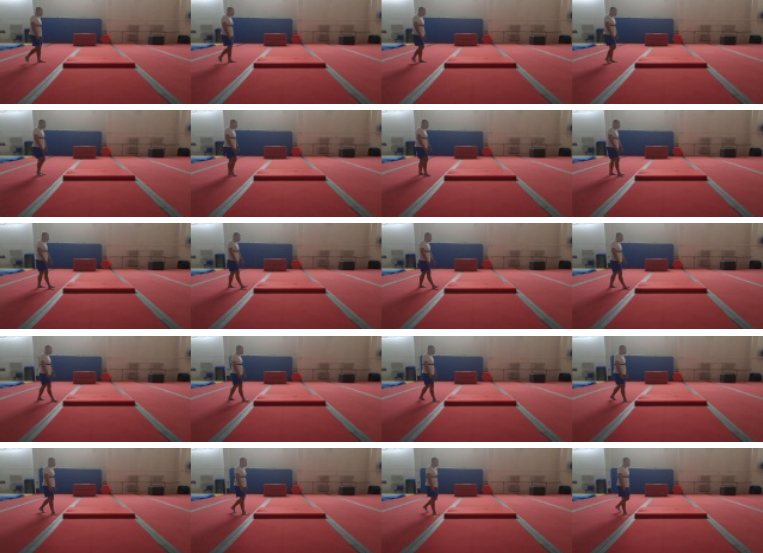
\includegraphics[width=0.5\linewidth]{./imgs/ds-sample-1.png}
    \caption{Imagens de um vídeo da base de dados \textit{Fall Video Dataset}.}
    \label{fig:ds-sample-1}
\end{figure}

Outras duas bases de dados foram utilizadas para o processo de treinamento da rede neural convolucional. Uma base de dados foi utilizada exclusivamente para cálculo das métricas de validação e o outra base de dados foi utilizada para cálculo das métricas de teste. A base de dados utilizada na validação é conhecida como GMDCSA-24 \citep{Alam2024GMDCSA24}. Essa base de dados conta com 6.988 vídeos de pequena duração que foram registrados em ambientes domésticos com simulação de atividades rotineiras como de andar, pegar, sentar e assim por diante. No entanto, diferente da base de dados \textit{Fall Video Dataset}, os vídeos da base de dados GMDCSA-24 apresentam cenas maiores e mais complexas de modo que seu uso direto no processo de validação durante o treinamento não foi possível. Para adequá-la ao \textit{pipeline} de treinamento, uma intervenção manual foi necessária. Assim, usando o software de edição de vídeos Kdenlive, foi possível obter vídeos menores (clips) de cenas focadas em situação de queda ou de não queda. O trabalho dessa atividade comprometeu substancialmente a quantidade de dados disponíveis na validação.

A outra base de dados utilizada foi a \textit{Le2i Fall Dataset} \citep{charfi2013fall}. Essa base de dados reuni vídeos de situações de queda e de não queda em ambientes reais de cafeteria, casa e escritório. Em termos de composição das cenas contidas nos vídeos, a base de dados \textit{Le2i Fall Dataset} é semelhante a base de dados GMDCSA-24. Dessa maneira, a utilização da base de dados \textit{Le2i Fall Dataset} no processo de teste tradicional se apresentou inviável. Essa restrição foi contornada a partir da flexibilização dos procedimentos de teste pela simulação de um situação real da aplicação com visualização das classificações realizadas pela rede neural (detalhes apresentados nas próximas seções). Imagens de ambas as bases de dados são apresentadas na \textbf{Figura \ref{fig:ds-samples-2-3}}.

\begin{figure}[H]
    \centering
    \begin{subfigure}[b]{0.45\linewidth}
        \centering
        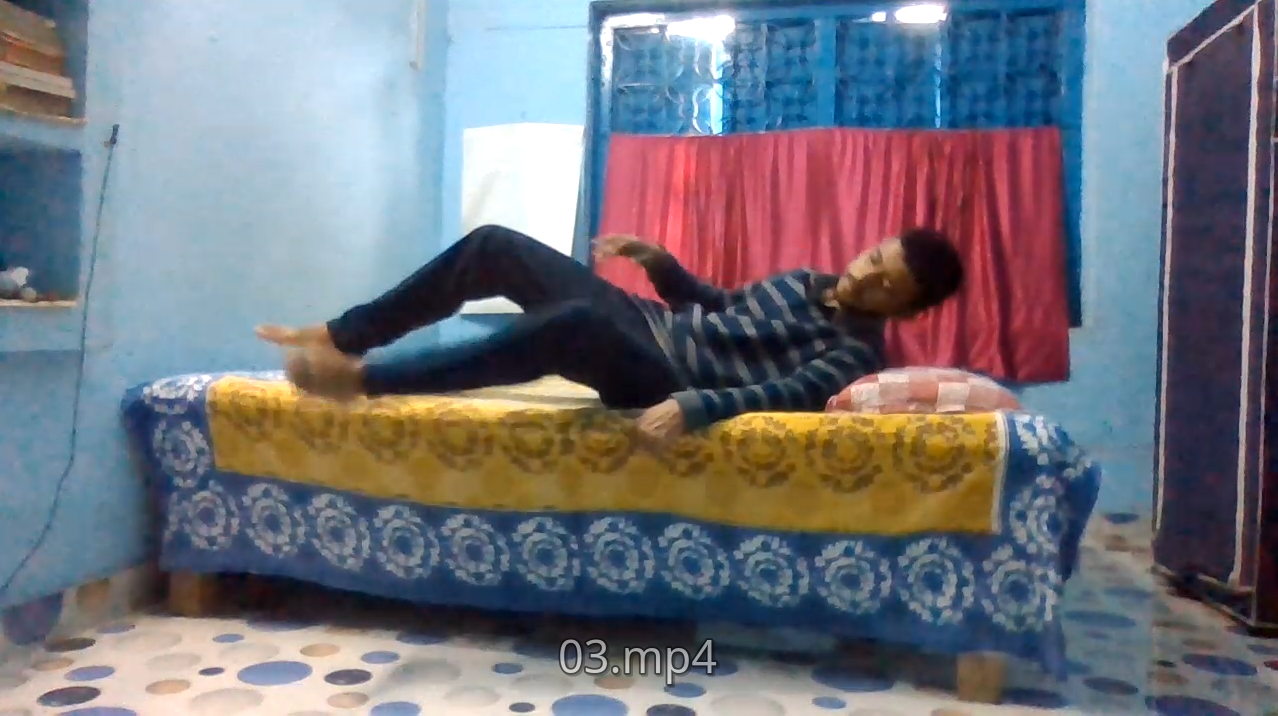
\includegraphics[width=\linewidth]{./imgs/ds-sample-2.png}
        \caption{Imagem de um vídeo da base de dados GMDCSA-24.}
        \label{fig:ds-sample-2}
    \end{subfigure}
    \hspace{0.05\linewidth}
    \begin{subfigure}[b]{0.45\linewidth}
        \centering
        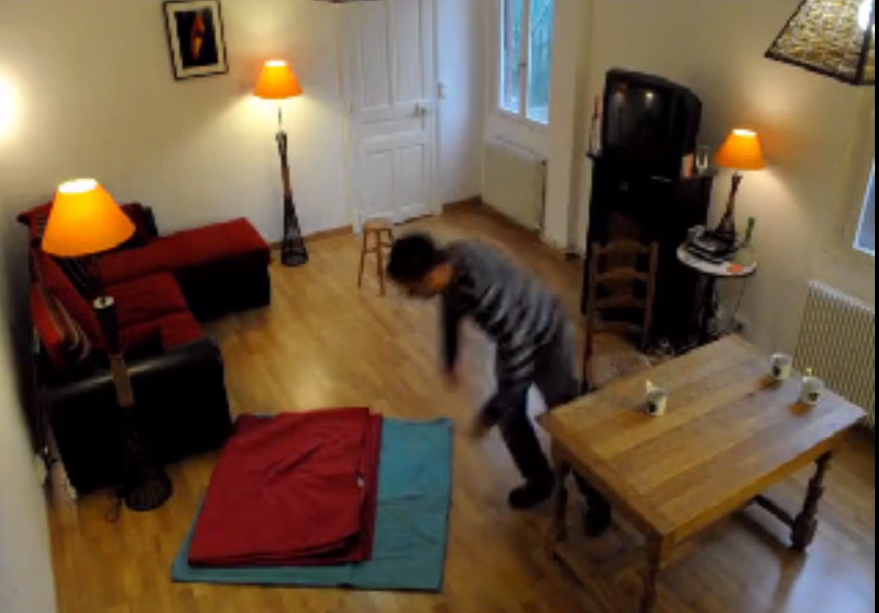
\includegraphics[width=\linewidth]{./imgs/ds-sample-3.png}
        \caption{Imagem de um vídeo da base de dados \textit{Le2i Fall Dataset}.}
        \label{fig:ds-sample-3}
    \end{subfigure}
    \caption{Imagem de um vídeo da base de dados GMDCSA-24 e \textit{Le2i Fall Dataset}.}
    \label{fig:ds-samples-2-3}
\end{figure}
%
%
\section{Metodologia}\label{sec:meto}
Nesta seção é apresentado os procedimentos e metodologias utilizados para o desenvolvimento do detector de queda. Assim, são abordados todos os elementos formadores do processo de treinamento da rede neural convolucional. Essa abordagem é feita nas seções de: pré-processamento e de modelo, otimizador e função de perda;

%
%
\subsection{Pré-processamento}\label{subsec:pre-proc}
Nesta seção são apresentados os assuntos relativos os processos de pré-processamento de dados realizados sobre as bases de dados para transformar os vídeos originais em imagens apropriadas para realização do treinamento da rede convolucional. Falaremos dos pré-processamentos específicos de transformação de vídeo em uma imagem, dos pré-processamentos específicos da YOLO (referentes à restrições do modelo e à aumentação de dados), e de um discussão preliminar acercar de assuntos relevantes ao escopo dessa seção.
%
%
\subsubsection{Pré-processamento: do vídeo para imagem}\label{subsubsec:pre-proc-1}
Para fazer o treinamento da rede neural convolucional do detector de queda, o evento de queda ou de não queda contido na cena registrada em cada vídeo das bases de dados \citep{payutch2025, Alam2024GMDCSA24, charfi2013fall} precisa ser codificado em uma única imagem. Isto é, para cada vídeo é necessário dispor de uma imagem que codifica a situação (de queda ou de não queda) registrada nele. 

A codificação da situação de queda ou de não queda registradas nos vídeos é realizada pela composição de uma imagem que contém uma sequência de imagens “menores” focadas apenas na pessoa presente no vídeo. A identificação da pessoa no vídeo para geração das imagens “menores” é realizada pela aplicação do modelo de detecção YOLO11L (versão 11 do modelo grande de detecção da YOLO) \citep{ultralytics2025}. 

Essas imagens “menores” foram geradas de uma subamostragem da quantidade total de frames do vídeo de trabalho. Elas foram geradas na quantidade máxima de até 15 imagens. Para todo vídeo com menos de 15 frames, todas as imagens “menores” foram salvas. Para vídeos com mais de 15 frames, foram salvas exatamente 15 imagens “menores” a partir de intervalos igualmente espaçados do início ao fim do vídeo. As imagens “menores” foram salvas nas dimensões de 100 por 100 pixels. Um exemplo de imagens “menores” geradas a partir do vídeo cujos frames estão mostrados na \textbf{Figura \ref{fig:ds-sample-1}} é apresentado na \textbf{Figura \ref{fig:ds-preproc-1}}.

\begin{figure}[H]
    \centering
    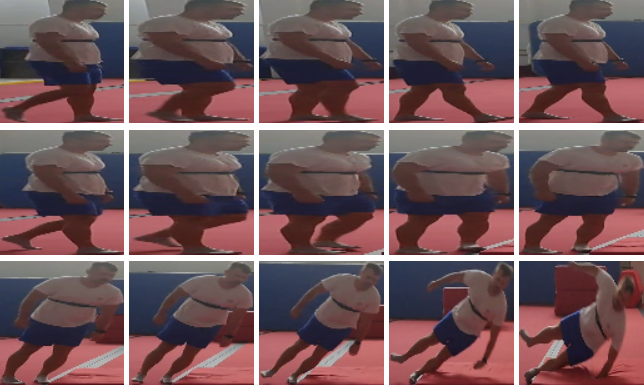
\includegraphics[width=0.5\linewidth]{./imgs/ds-preproc-1.png}
    \caption{Sequência de 15 imagens “menores” \ nas dimensões de 100 por 100 pixels de uma pessoa em condição de queda provenientes de um vídeo da base de dados \textit{Fall Video Dataset}.}
    \label{fig:ds-preproc-1}
\end{figure}

A partir da disponibilidade das imagens “menores”, a composição das imagens que codificam a condição de queda ou de não queda pôde ser realizada. Duas estratégias de composição são utilizadas. A primeira estratégia consiste em organizar as imagens “menores” em uma distribuição horizontal como mostrado na \textbf{Figura \ref{fig:ds-preproc-horiz-1}}.

\begin{figure}[H]
    \centering
    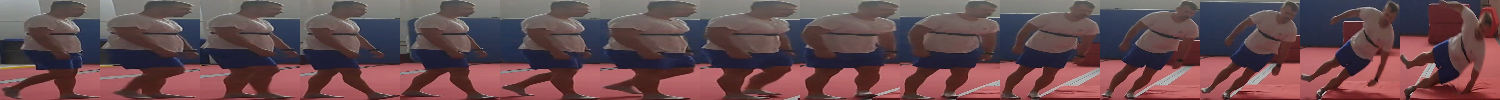
\includegraphics[width=0.99\linewidth]{./imgs/ds-preproc-horiz-1.png}
    \caption{Composição horizontal das imagens “menores” para codificação da condição de queda (ou de não queda).}
    \label{fig:ds-preproc-horiz-1}
\end{figure}

A segunda estratégia para composição das imagens consiste em organizar as imagens “menores” em uma distribuição matricial a partir de um ordenamento baseado primeiro na direção da esquerda para a direita e depois na direção de cima para baixo. Essa distribuição matricial é apresentada na \textbf{Figura \ref{fig:ds-preproc-matr-1}}.

\begin{figure}[H]
    \centering
    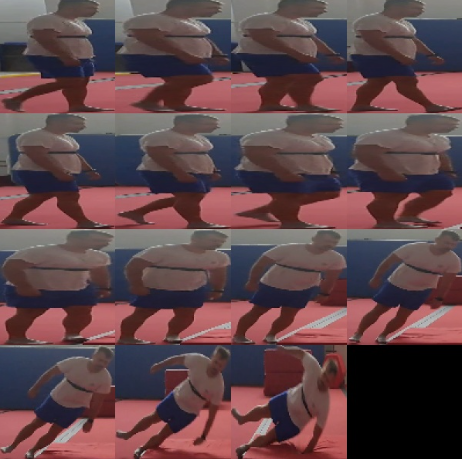
\includegraphics[width=0.5\linewidth]{./imgs/ds-preproc-matr-1.png}
    \caption{Composição matricial das imagens “menores” para codificação de queda (ou de não queda).}
    \label{fig:ds-preproc-matr-1}
\end{figure}
%
%
\subsubsection{Pré-processamento: da imagem para a YOLO}\label{subsubsec:pre-proc-2}
Como utilizamos a arquitetura de redes convolucionais desenvolvida pelo grupo Ultralyrics, as imagens compostas utilizadas para treinamento da rede neural estão submetidas às restrições do modelo YOLO. Em particular, o modelo de classificação apresenta uma limitação relevante para esse trabalho: as imagens de entrada precisam ter dimensões de mesmo tamanho (o aspecto da imagem precisa ser quadrado). 

Devido a essa especificidade do modelo da YOLO, as imagens de treinamento, no momento exatamente antes ao processo de alimentar a rede neural (\textit{feedforward}), foram transformadas em quadrados a partir do aumento de tamanho da menor dimensão na medida necessária para deixar a imagem com aspecto quadrado. A área adicionada na imagem pelo aumento da dimensão foi preenchida com a cor preta (valor 0). Para a estratégia de composição horizontal das imagens, o resultado do ajuste da imagem para o aspecto quadrado é mostrado na \textbf{Figura \ref{fig:ds-preproc-yolo-horiz-1}}.

\begin{figure}[H]
    \centering
    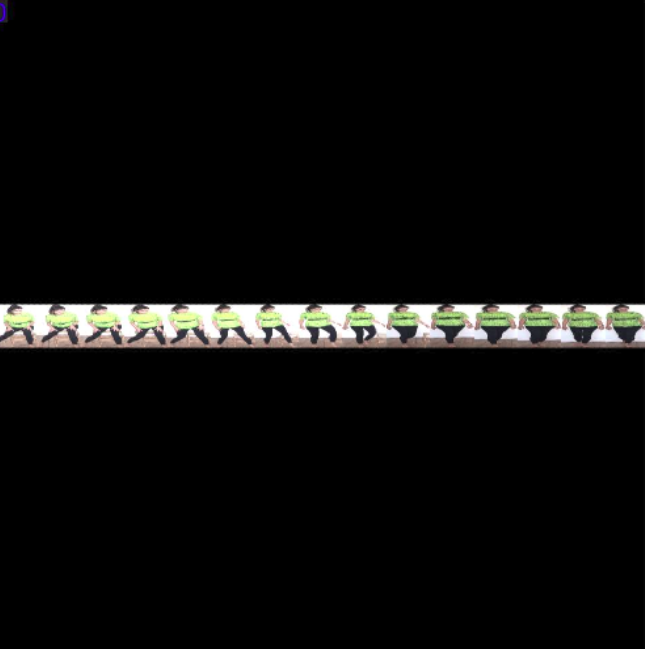
\includegraphics[width=0.5\linewidth]{./imgs/ds-preproc-yolo-horiz-1.png}
    \caption{Resultado do ajuste da imagem em composição horizontal para o aspecto quadrado.}
    \label{fig:ds-preproc-yolo-horiz-1}
\end{figure}

Para a estratégia de composição matricial das imagens, o resultado é apresentado na \textbf{Figura \ref{fig:ds-preproc-yolo-matr-1}} (neste caso a imagem já apresenta dimensão quadrada).

\begin{figure}[H]
    \centering
    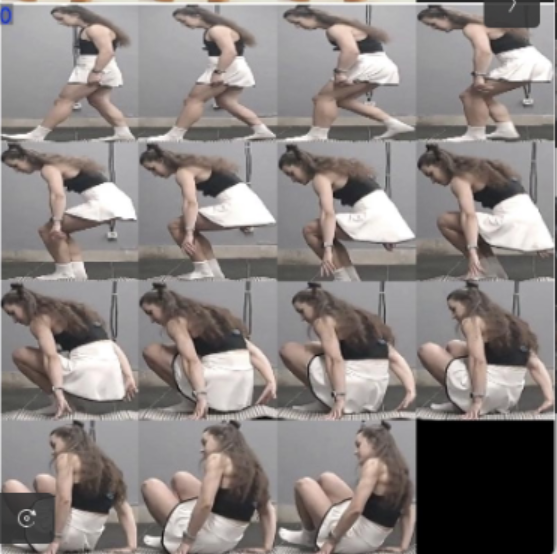
\includegraphics[width=0.5\linewidth]{./imgs/ds-preproc-yolo-matr-1.png}
    \caption{Resultado do ajuste da imagem em composição matricial para o aspecto quadrado.}
    \label{fig:ds-preproc-yolo-matr-1}
\end{figure}
%
%
\subsubsection{Pré-processamento: aumentação de dados}\label{subsubsec:pre-proc-3}
A importância da aumentação de dados em treinamentos de modelos de aprendizado de máquinas e redes neurais é senso comum dentro da comunidade de inteligência artificial. Posicionado como um procedimento relevante dentro dos artifícios e estratégias utilizadas no processo de orientar o modelo para um condição de generalização adequada de modo a evitar a conhecida condição de \textit{overfitting}, a aumentação de dados está geralmente presente na grande maioria dos \textit{pipelines} de treinamentos de modelos de inteligência artificial. Neste trabalho os procedimentos de aumentação de dados utilizados foram de rotação, recorte, e alteração de cor, brilho e contraste (\textbf{Figura \ref{fig:aumentacao-1-3}}). 

\begin{figure}[H]
    \centering
    \begin{subfigure}[b]{0.3\linewidth}
        \centering
        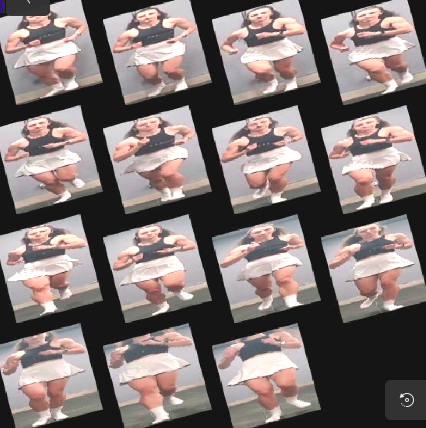
\includegraphics[width=\linewidth]{./imgs/aumentacao-1.png}
        \caption{Rotação.}
        % \label{fig:ds-sample-1}
    \end{subfigure}
    \hspace{0.03\linewidth}
    \begin{subfigure}[b]{0.3\linewidth}
        \centering
        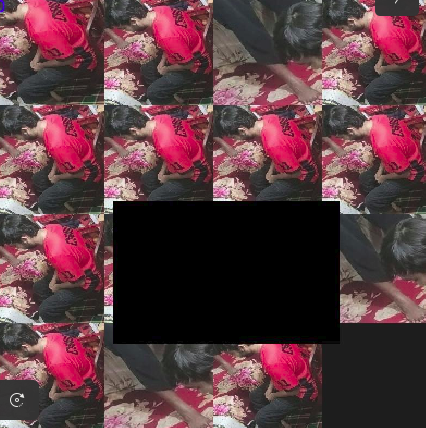
\includegraphics[width=\linewidth]{./imgs/aumentacao-2.png}
        \caption{Recorte.}
        % \label{fig:ds-sample-2}
    \end{subfigure}
    \hspace{0.03\linewidth}
    \begin{subfigure}[b]{0.3\linewidth}
        \centering
        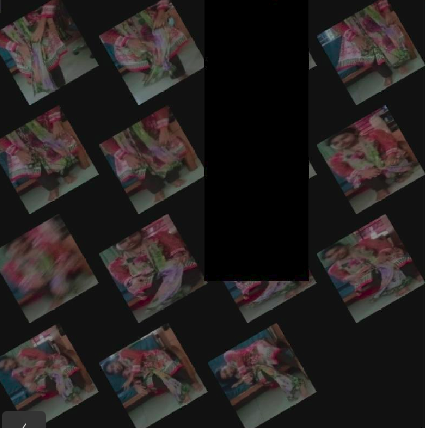
\includegraphics[width=\linewidth]{./imgs/aumentacao-3.png}
        \caption{Cor, brilho e contraste.}
        % \label{fig:ds-sample-3}
    \end{subfigure}
    \caption{Aumentação de dados de rotação, recorte e alteração de cor, brilho e contraste.}
    \label{fig:aumentacao-1-3}
\end{figure}
%
%
\subsubsection{Pré-processamento: discussão preliminar}\label{subsubsec:pre-proc-3}
Nesta seção foram apresentados os elementos relativos as atividades de pré-processamento de imagens. Desses elementos, é importante pontuar que a composição da imagem “maior” a partir das imagens “menores” da pessoa detectada na moldura horizontal foi uma primeira iniciativa de organização das imagens para o treinamento. Essa composição não se mostrou adequada em termos de eficiência, tamanho final da imagem e desempenho da rede treinada. A estrutura horizontal apresentou grande ineficiência de organização da informação porque a imagem “maior” resultante tem mais áreas de não informação (pixel 0) do que de informação (pixels de outros valores formadores da imagem). O imagem “maior” resultante apresentou dimensões finais demasiadas grandes (1200x1200 pixels) devido a necessidade de acomodar todas as 15 imagens “menores” em uma dimensão mínima razoável que no caso deste trabalho foi de 80x80 pixels (\textbf{Figura \ref{fig:ds-preproc-yolo-horiz-1}}). O desempenho da rede neural treinada foi ligeiramente abaixo das expectativas. Diante dessas desvantagem, a composição matricial (\textbf{Figura \ref{fig:ds-preproc-yolo-matr-1}}) foi escolhida para uso durante todas as demais experimentações de treinamento realizadas neste trabalho. 
%
%
\subsection{Modelo, otimizador e função de perda}\label{subsec:model}
Apresentamos uma breve visão teórica do modelo, do otimizador e da função de perda utilizados.

\subsubsection{Modelo}\label{subsubsec:model}
A unidade central de sustentação do sistema de detecção de queda de pessoa é uma rede neural convolucional disponibilizada pelo grupo Ultralytics \citep{ultralytics2025}. Redes neurais convolucionais formam um grupo de redes neurais de arquiteturas que apresentam como operação principal a convolução \citep{lecun1998gradient}. A convolução quando aplicada no contexto de redes neurais e imagens - matrizes com informações correlacionadas por localidade - apresenta a vantagem de eficiência computacional (a organização dos neurônios da rede acontece de uma maneira que no final há uma totalização de parâmetros menor do que a totalização de parâmetros de redes neurais tradicionais) e a vantagem de possuir a capacidade de considerar no seu processo de cálculo matemático as informações de localidade naturalmente presentes nas cenas registradas em imagens.

Além da operação de convolução, outro elemento constituinte importante das redes neurais convolucionais é o filtro. O filtro é uma matriz de pesos cujos melhores valores serão aprendidos durante o processo de treinamento. O filtro é utilizado na convolução junto com a imagem. Esse filtro, ao longo do treinamento vai adquirindo pesos capazes de extrair informações da imagens que são relevantes para problemas de classificação, detecção e segmentação (entre outros). Uma exemplo ilustrativo de um possível filtro a ser aprendido por uma rede neural convolucional é o de detecção de cantos apresentando da \textbf{Figura \ref{fig:cnn-filtro}}.

\begin{figure}[H]
    \centering
    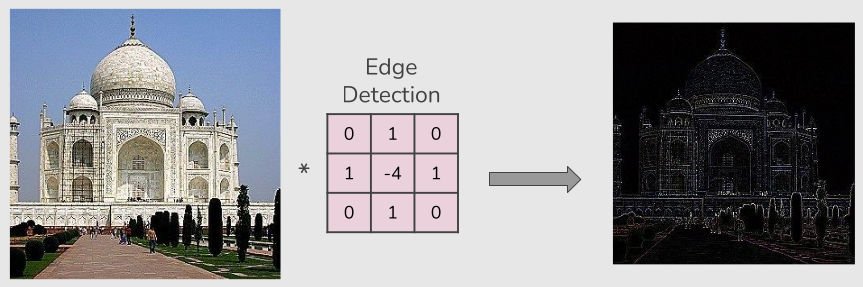
\includegraphics[width=0.99\linewidth]{./imgs/cnn-filtro.png}
    \caption{Ilustração de aplicação de convolução com filtro de detecção de cantos sobre imagem.}
    \label{fig:cnn-filtro}
\end{figure}

A matriz resultante da aplicação do filtro é chamada de mapa de ativação. Cada filtro gera um mapa de ativação e em cada etapa de convolução de uma rede neural convolucional ocorre a aplicação de vários filtros e geração de vários mapas de ativação. Esses mapas de ativação, por sua vez, são utilizados em convoluções seguintes que utilizam outros filtros (\textbf{Figura \ref{fig:cnn-ativacao}}). 

\begin{figure}[H]
    \centering
    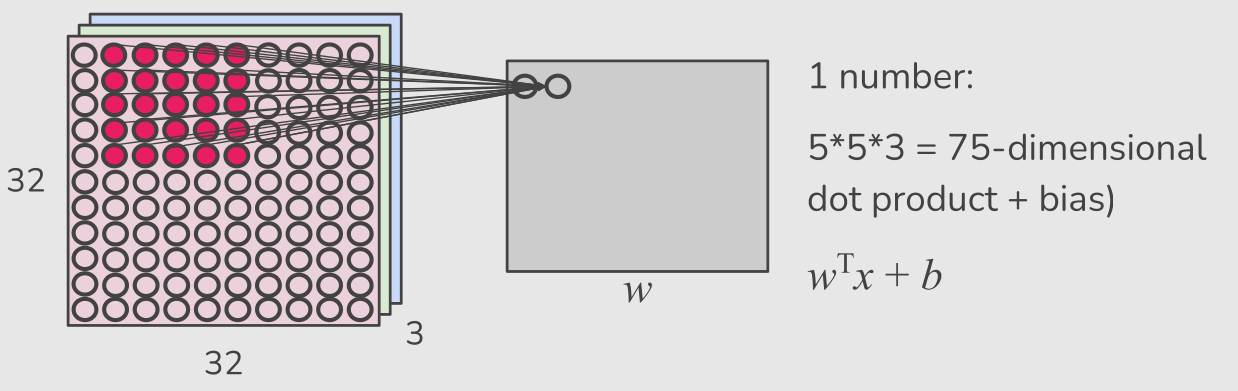
\includegraphics[width=0.99\linewidth]{./imgs/cnn-ativacao.png}
    \caption{Ilustração de aplicação de um filtro sobre uma imagem a partir da convolução com geração de um mapa de ativação.}
    \label{fig:cnn-ativacao}
\end{figure}

O conjunto convolução, mapas de ativação, filtros e outros elementos (\textit{pooling}, \textit{drop-out}, função de ativação) é formador da arquitetura de redes neurais convolucionais. Na \textbf{Figura \ref{fig:cnn-exemplo}} temos um exemplo completo de rede neural convolucionais.

\begin{figure}[H]
    \centering
    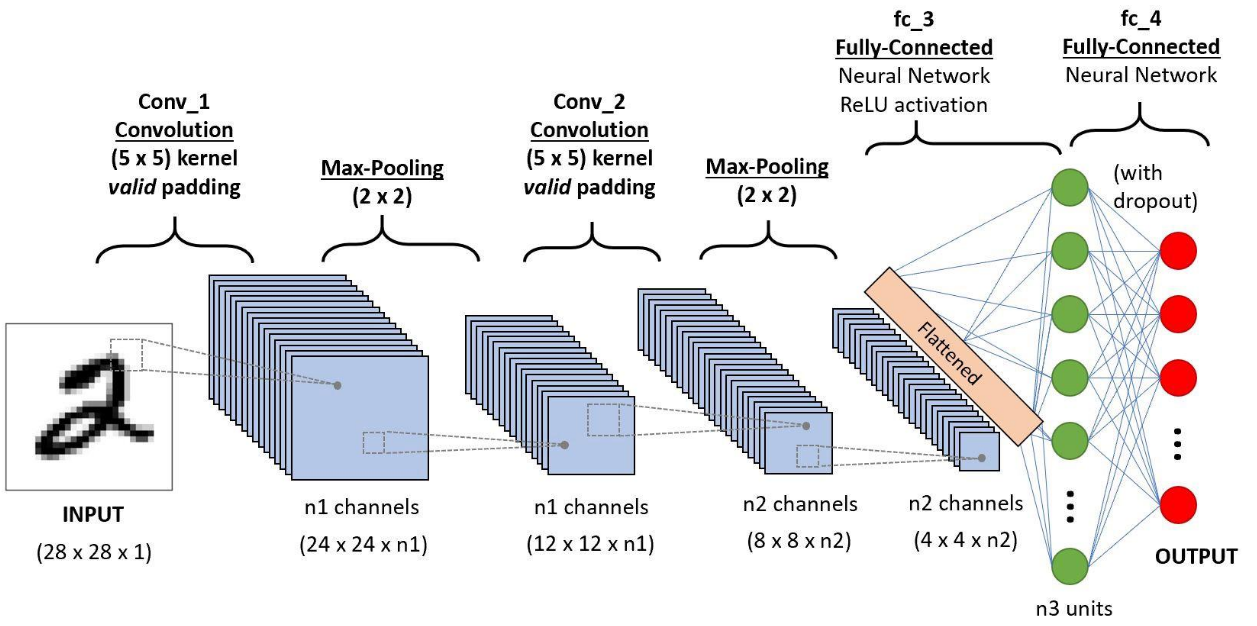
\includegraphics[width=0.99\linewidth]{./imgs/cnn-exemplo.png}
    \caption{Ilustração de rede neural convolucional.}
    \label{fig:cnn-exemplo}
\end{figure}

Para este trabalho, utilizou-se o modelo YOLO11N cujo resumo da arquitetura está apresentado na \textbf{Figura \ref{fig:cnn-yolo}}. Essa figura apresenta em alto nível os blocos formadores da arquitetura da YOLO11N. Para maiores detalhes sobre as especificidades desses blocos, recomenda-se procurar o repositório do grupo Ultralytics \citep{ultralytics2025}.

\begin{figure}[H]
    \centering
    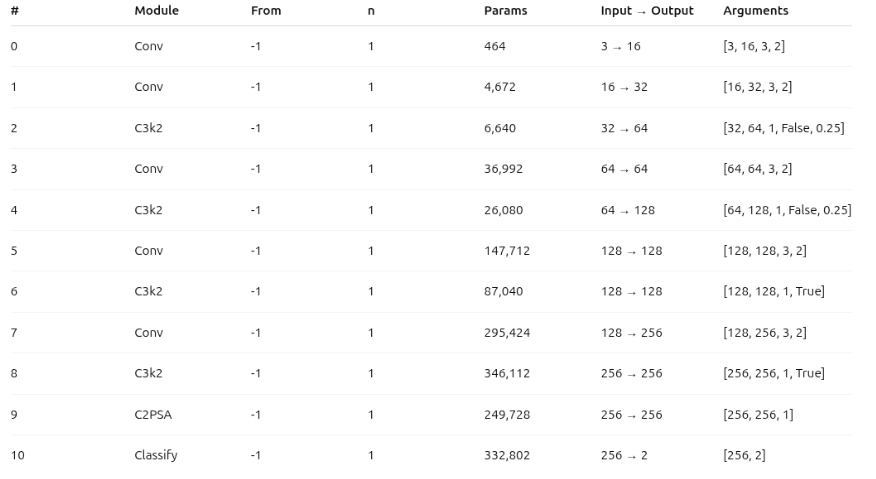
\includegraphics[width=0.99\linewidth]{./imgs/cnn-yolo.png}
    \caption{Arquitetura da YOLO11N.}
    \label{fig:cnn-yolo}
\end{figure}

\subsubsection{Otimizador}\label{subsubsec:otim}
Para o treinamento de redes neurais dois processos se destacam: um processo é chamado de \textit{feedforward} e o outro é de \textit{backpropagation}. No processo de \textit{feedforward} um conjunto de dados (\textit{batch}) é inserido na rede neural. Após processado, os erros cometidos pela rede sobre os dados de alimentação são calculados. A maneira que esse cálculo é realizado para composição de um único valor representativo da qualidade de inferência da rede neural é determinada pela função de perda. É a partir dos valores da função de perda que é possível definir quais modificações podem ser feitas nos pesos da rede neural de forma que ela melhore (aprenda) a qualidade da sua inferência. De forma mais técnica, as modificações realizadas nos pesos da rede em treinamento são dirigidas pelos valores do vetor gradiente que é calculado a partir da aplicação de derivadas sobre a função de perda dentro do que é conhecido como um problema de otimização \citep{boyd2004convex}. A atualização dos pesos da rede neural a partir dos valores do gradiente e do algoritmo de otimização é chamada de \textit{backpropagation}. Fica evidente que um elemento importante durante o treinamento de uma rede neural é o otimizador. Nesse trabalho usamos o otimização \textit{Stochastic Gradient Descent} (SGD) com momento \citep{robbins1951stochastic}. Uma visão geral das formalizações matemáticas do otimizador utilizado neste trabalho é apresentada na \textbf{Figura \ref{fig:cnn-sgd}}.

\begin{figure}[H]
    \centering
    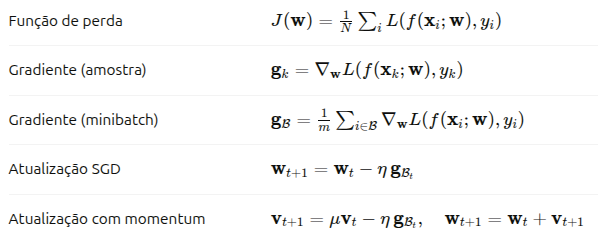
\includegraphics[width=0.80\linewidth]{./imgs/cnn-sgd.png}
    \caption{Formulação do \textit{Stochastic Gradient Descent} (SGD) com momento.}
    \label{fig:cnn-sgd}
\end{figure}

\subsubsection{Função de perda}\label{subsubsec:perda}
Um outro elemento importante no processo de treinamento de uma rede neural convolucional é a função de perda. A função de perda é a função utilizada para quantificar a qualidade das inferências da rede neural em treinamento a partir dos dados de entrada e a comparação das predições realizadas pela rede e as predições esperadas para os dados de entrada. Neste trabalho utilizamos a função de perda \textit{Cross Entropy Loss} cujas principais formulações são apresentadas na \textbf{Figura \ref{fig:cnn-perda}}.

\begin{figure}[H]
    \centering
    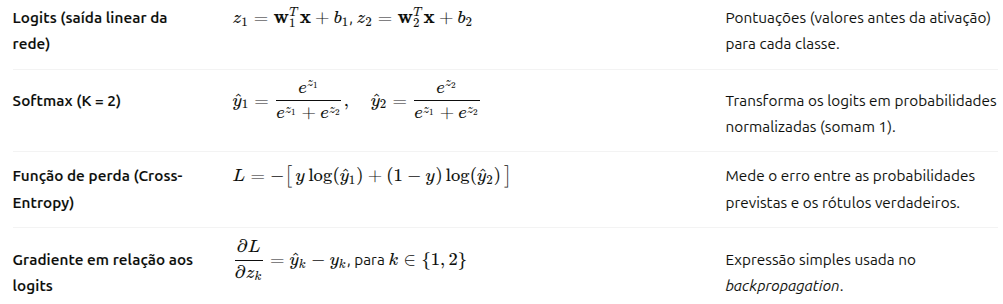
\includegraphics[width=0.80\linewidth]{./imgs/cnn-perda.png}
    \caption{Função de perda \textit{Cross Entropy Loss}.}
    \label{fig:cnn-perda}
\end{figure}


\section{Resultados}\label{sec:resu}
Os resultados deste trabalho são provenientes dos treinamentos realizados. Esses resultados são: identificação de condição de vazamento de dados; possível identificação de \textit{overfitting}; matrizes de confusão para todos os treinos, horas de treinaneto e, por fim, dentro de uma perspectiva qualitativa, desempenho do último modelo treinando sobre a base de dados de teste. As configurações padrões utilizadas em todos os treinamentos foram:
\begin{itemize}
    \item modelo YOLO11N do grupo Ultralytics;
    \item classificação binária com 0 para situação de não queda e 1 para situação de queda;
    \item \textit{batch} de tamanho 4 (número de imagens enviadas em cada etapa de \textit{feedforward});
    \item otimizador \textit{Stochastic Gradient Descent} com momento com valores de 0.09 de \textit{learning rate} e 0.9 de momento;
    \item 200 época;
    \item proporção de 0,8 para dados de treinamento e 0,2 para dados de teste.
\end{itemize}
Foram realizados 6 treinamentos cujas principais diferenças entre eles apresentam-se em mudanças nas estratégias de aumentação de dados ou na origem da própria base de dados. Uma amostra de um \textit{batch}, métricas de desempenho e uma matriz de confusão são apresentadas a seguir para cada treinamento.

\subsection{Treinamento 1 (ingênuo)}\label{sec:t1}
O treinamento 1 ou treinamento ingênuo foi o treinamento realizado utilizando as configurações padrões da YOLO. Esse treinamento permitiu perceber que a composição das imagens para o treinamento na estratégia horizontal apresentava as desvantagens de ter que utilizar uma imagem muito grande (1200x1200 pixels) para que as imagens memores mantivessem uma dimensão mínima adquada para manutenção das informações. Também foi possível perceber que aplicar a aumentação de dados de rotação integralmente sobre a imagem não fazia sentido dentro da maneira que o problema foi modelado e abordado (\textbf{Figura \ref{fig:t1-1}}).


\begin{figure}[H]
    \centering
    \begin{subfigure}[b]{0.45\linewidth}
        \centering
        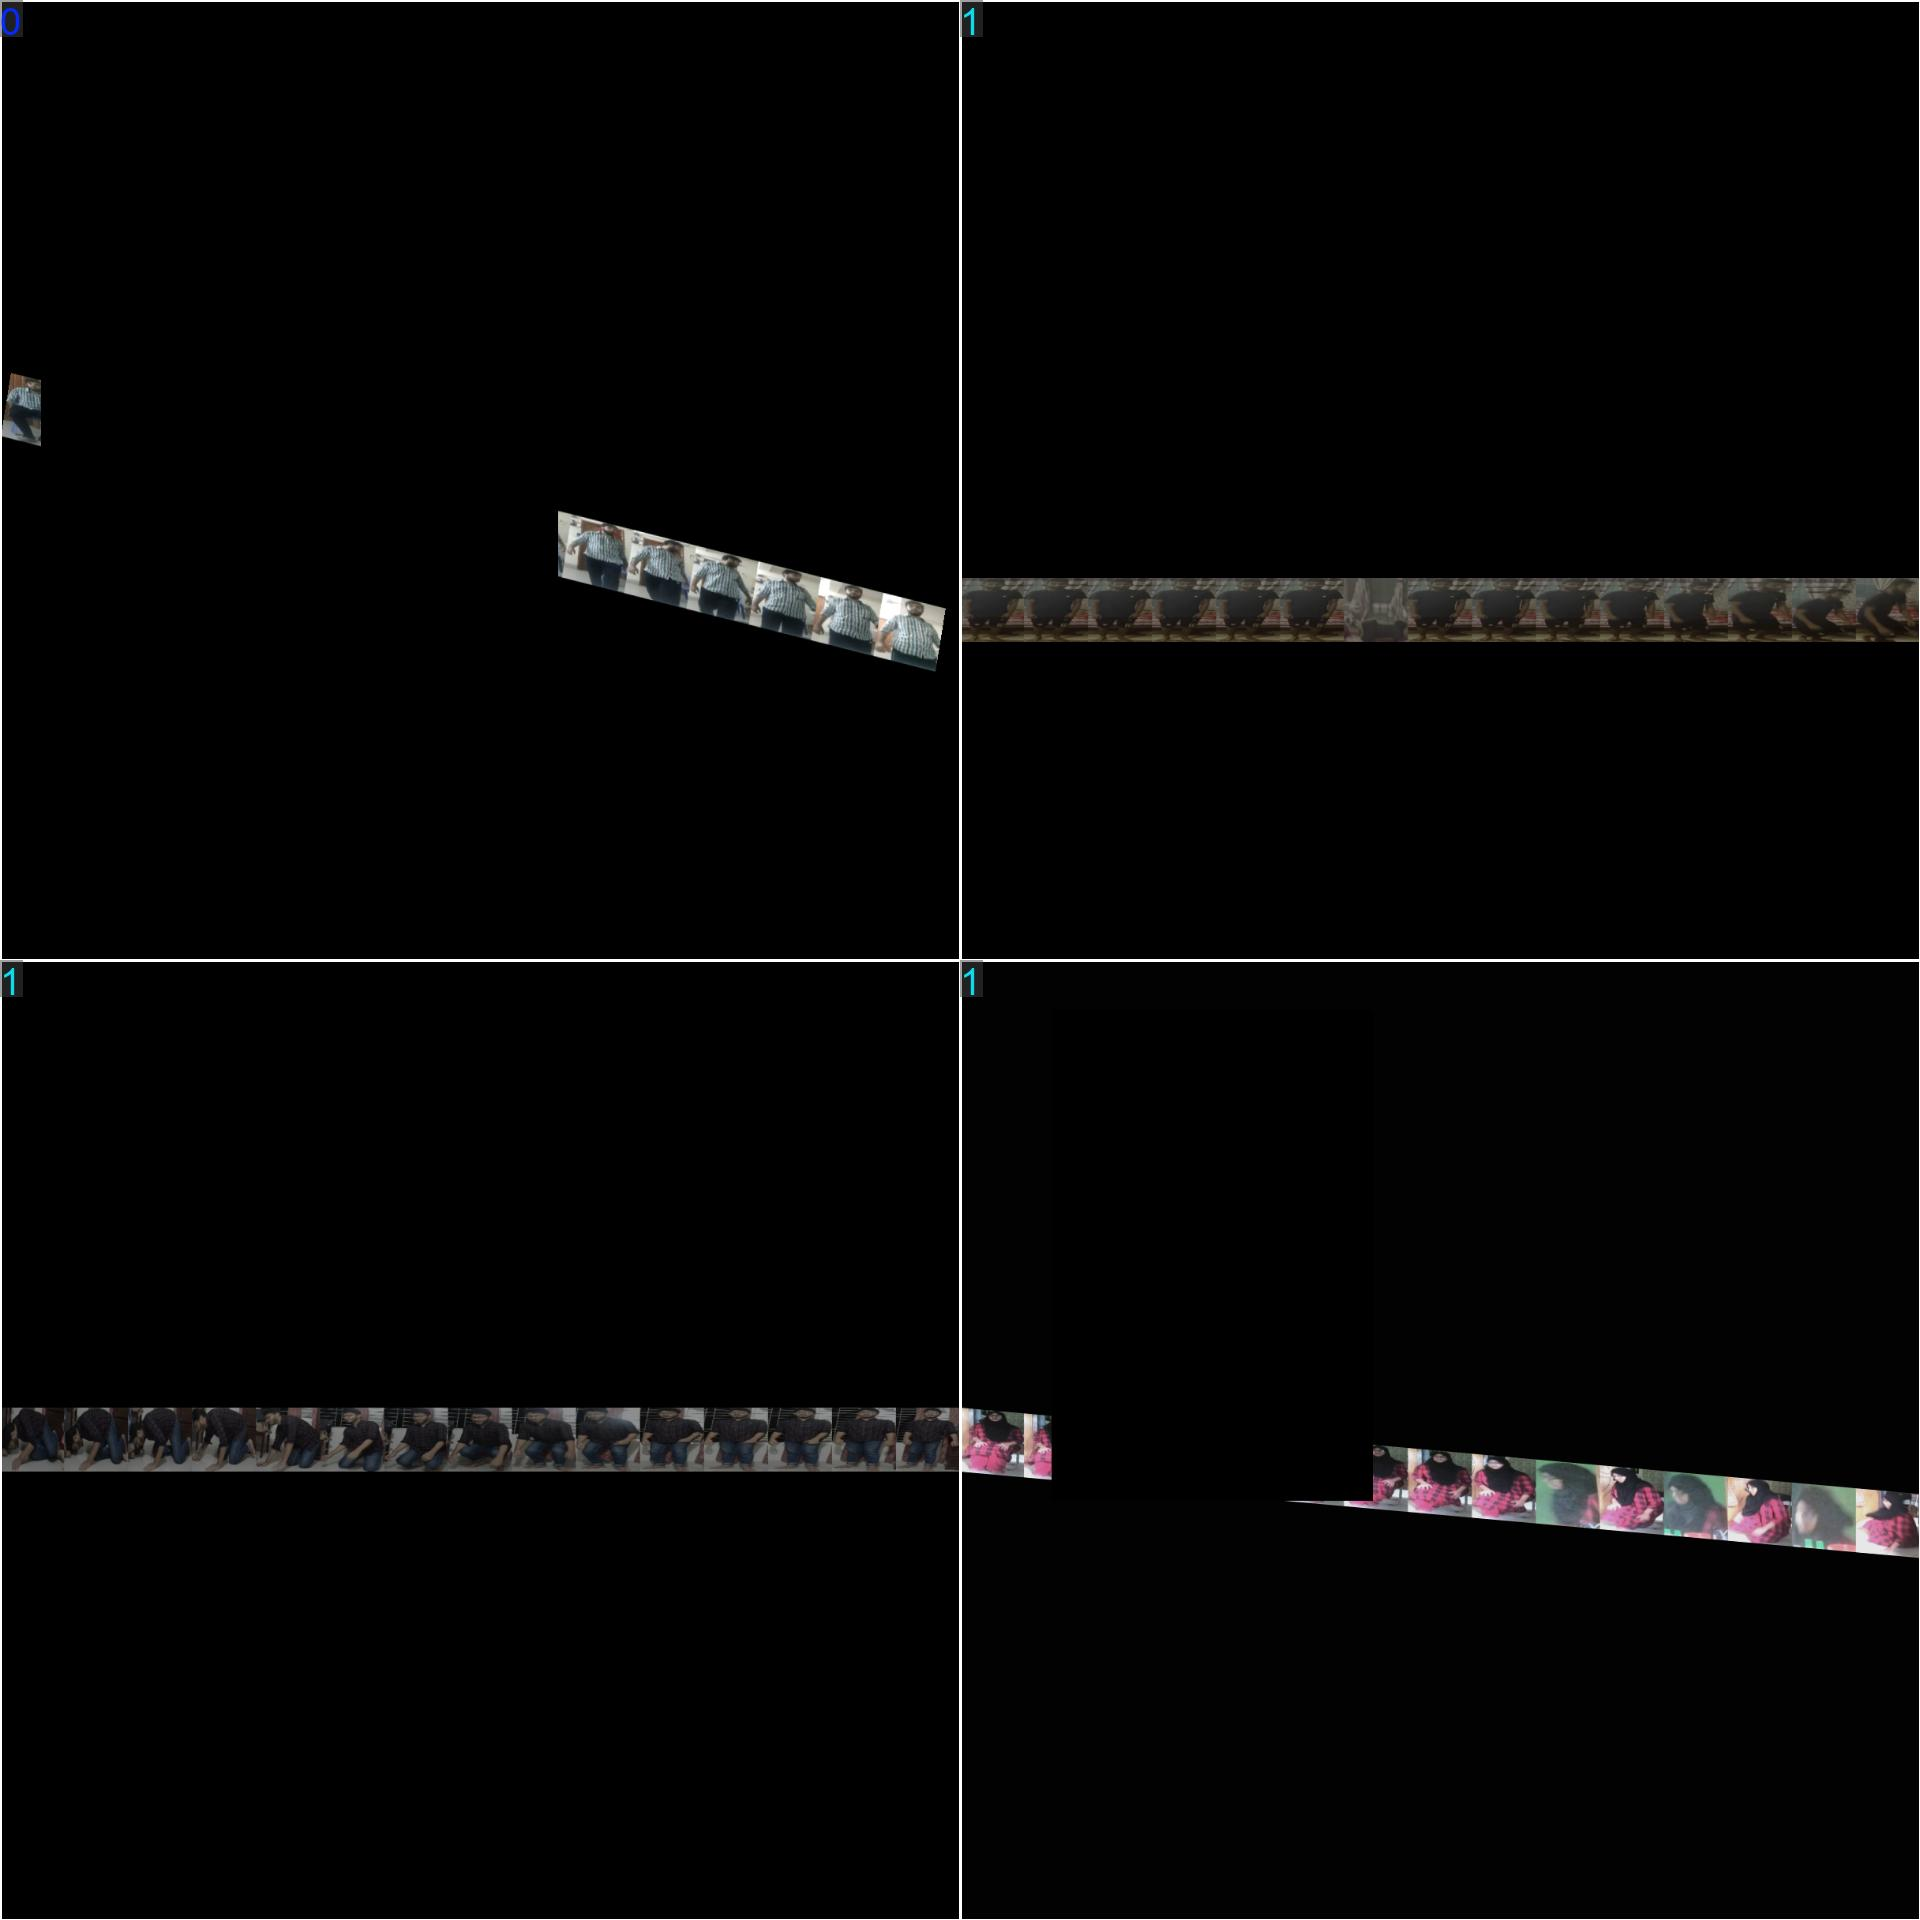
\includegraphics[width=\linewidth]{./imgs/t1-train_batch.jpg}
        \caption{Amostra de batch.}
    \end{subfigure}
    \hspace{0.05\linewidth}
    \begin{subfigure}[b]{0.45\linewidth}
        \centering
        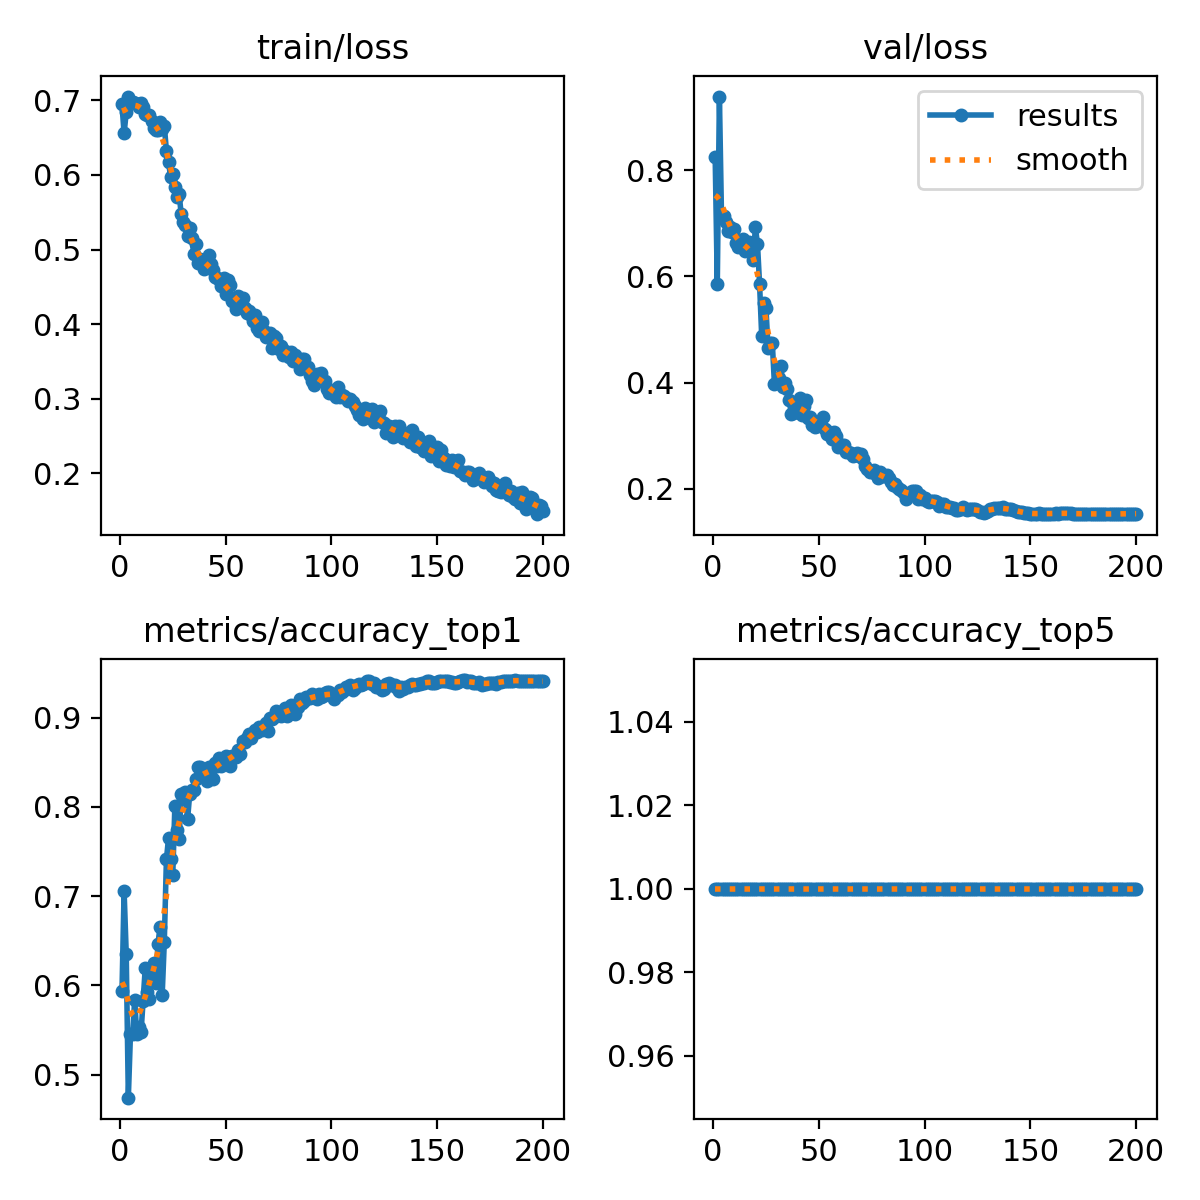
\includegraphics[width=\linewidth]{./imgs/t1-results.png}
        \caption{Métricas de desempenho.}
    \end{subfigure}
    \caption{Treinamento 1: amostra de batch e métricas de desempenho.}
    \label{fig:t1-1}
\end{figure}

Sobre o comportamento das métricas de desempenho, verifica-se que sua evolução obedeceu um padrão canônico de diminuição gradual em formato de uma exponência. A métrica de acurária também apresentou uma evolução adequada (\textbf{Figura \ref{fig:t1-1}}).

\begin{figure}[H]
    \centering
    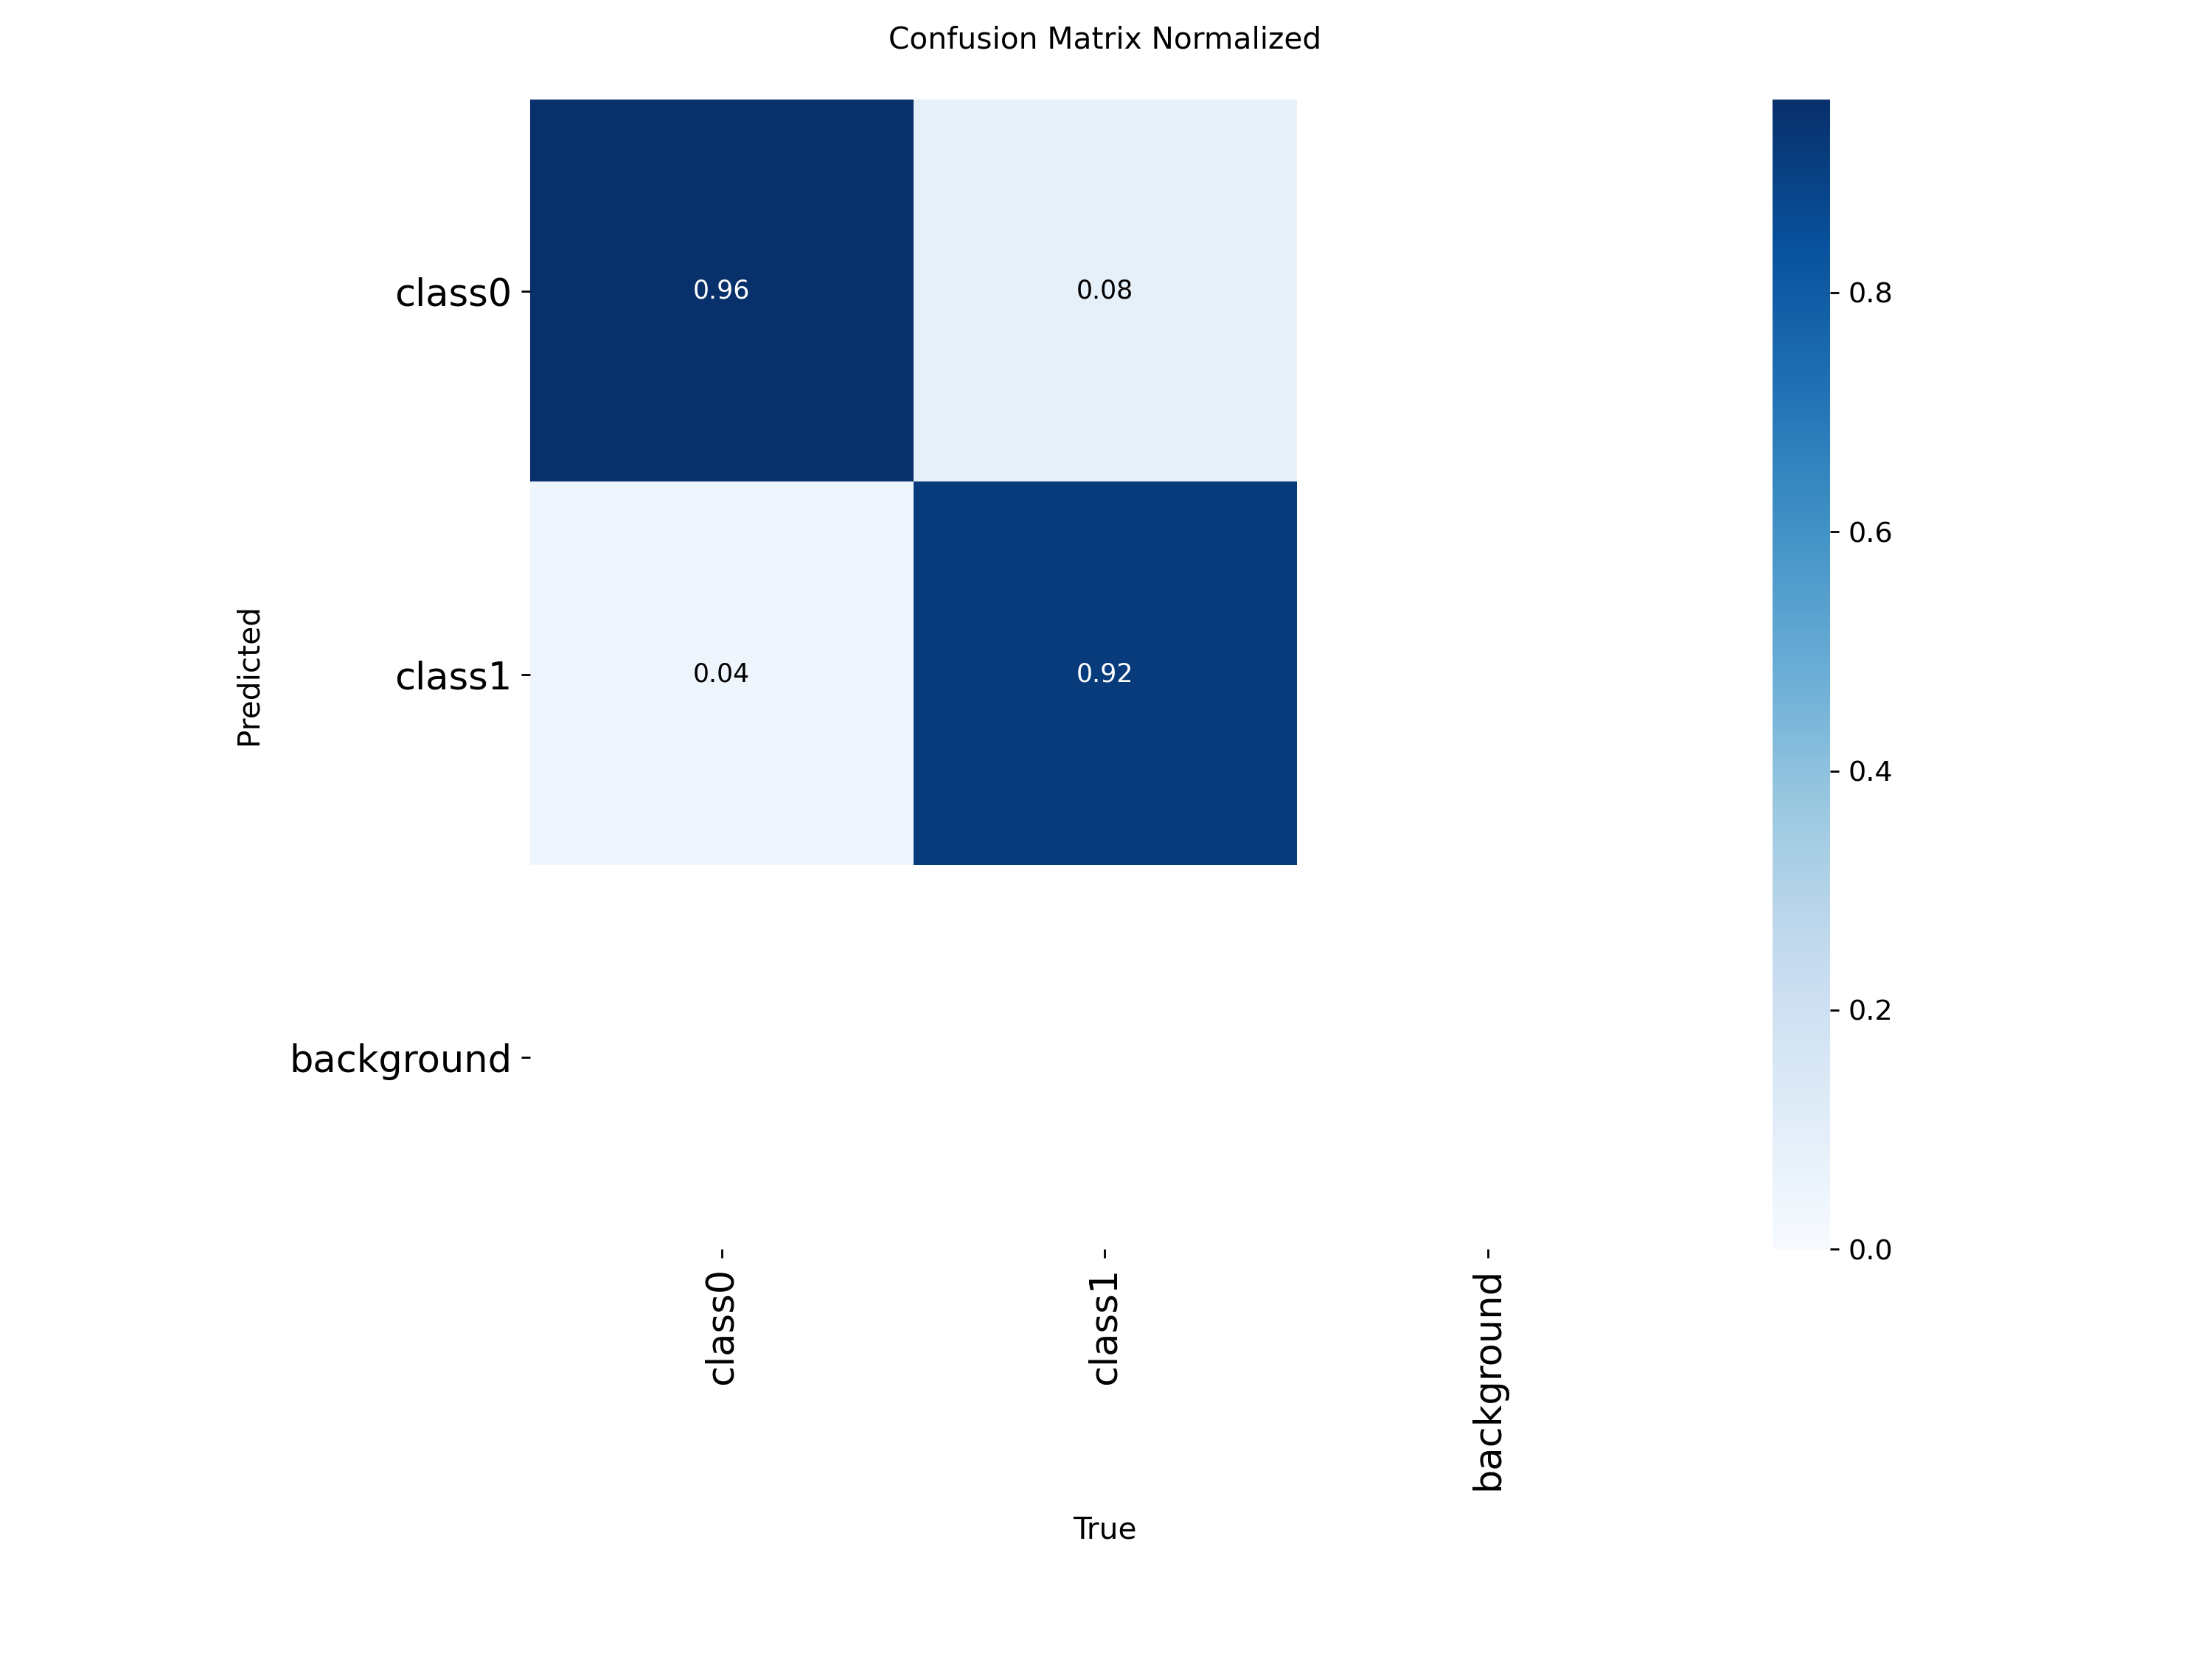
\includegraphics[width=0.80\linewidth]{./imgs/t1-confusion_matrix_normalized.png}
    \caption{Treinamento 1: matriz de confusão normalizada.}
    \label{fig:t1-2}
\end{figure}

A matriz de confusão normalizada demonstra que o modelo dentro do espaço amostral varrido pelas bases de dados foi capaz de aprender de maneira satisfatório os padrões associados a situação de queda e situações de não queda (\textbf{Figura \ref{fig:t1-2}}).


\subsection{Treinamento 2}\label{sec:t2}
Neste treinamento, a composição das imagens ainda foi realizada a partir da moldura horizontal. A diferença desse treinamento em relação ao anterior foi a removeção da aumentação de dados de rotação (\textbf{Figura \ref{fig:t2-1}}).

\begin{figure}[H]
    \centering
    \begin{subfigure}[b]{0.45\linewidth}
        \centering
        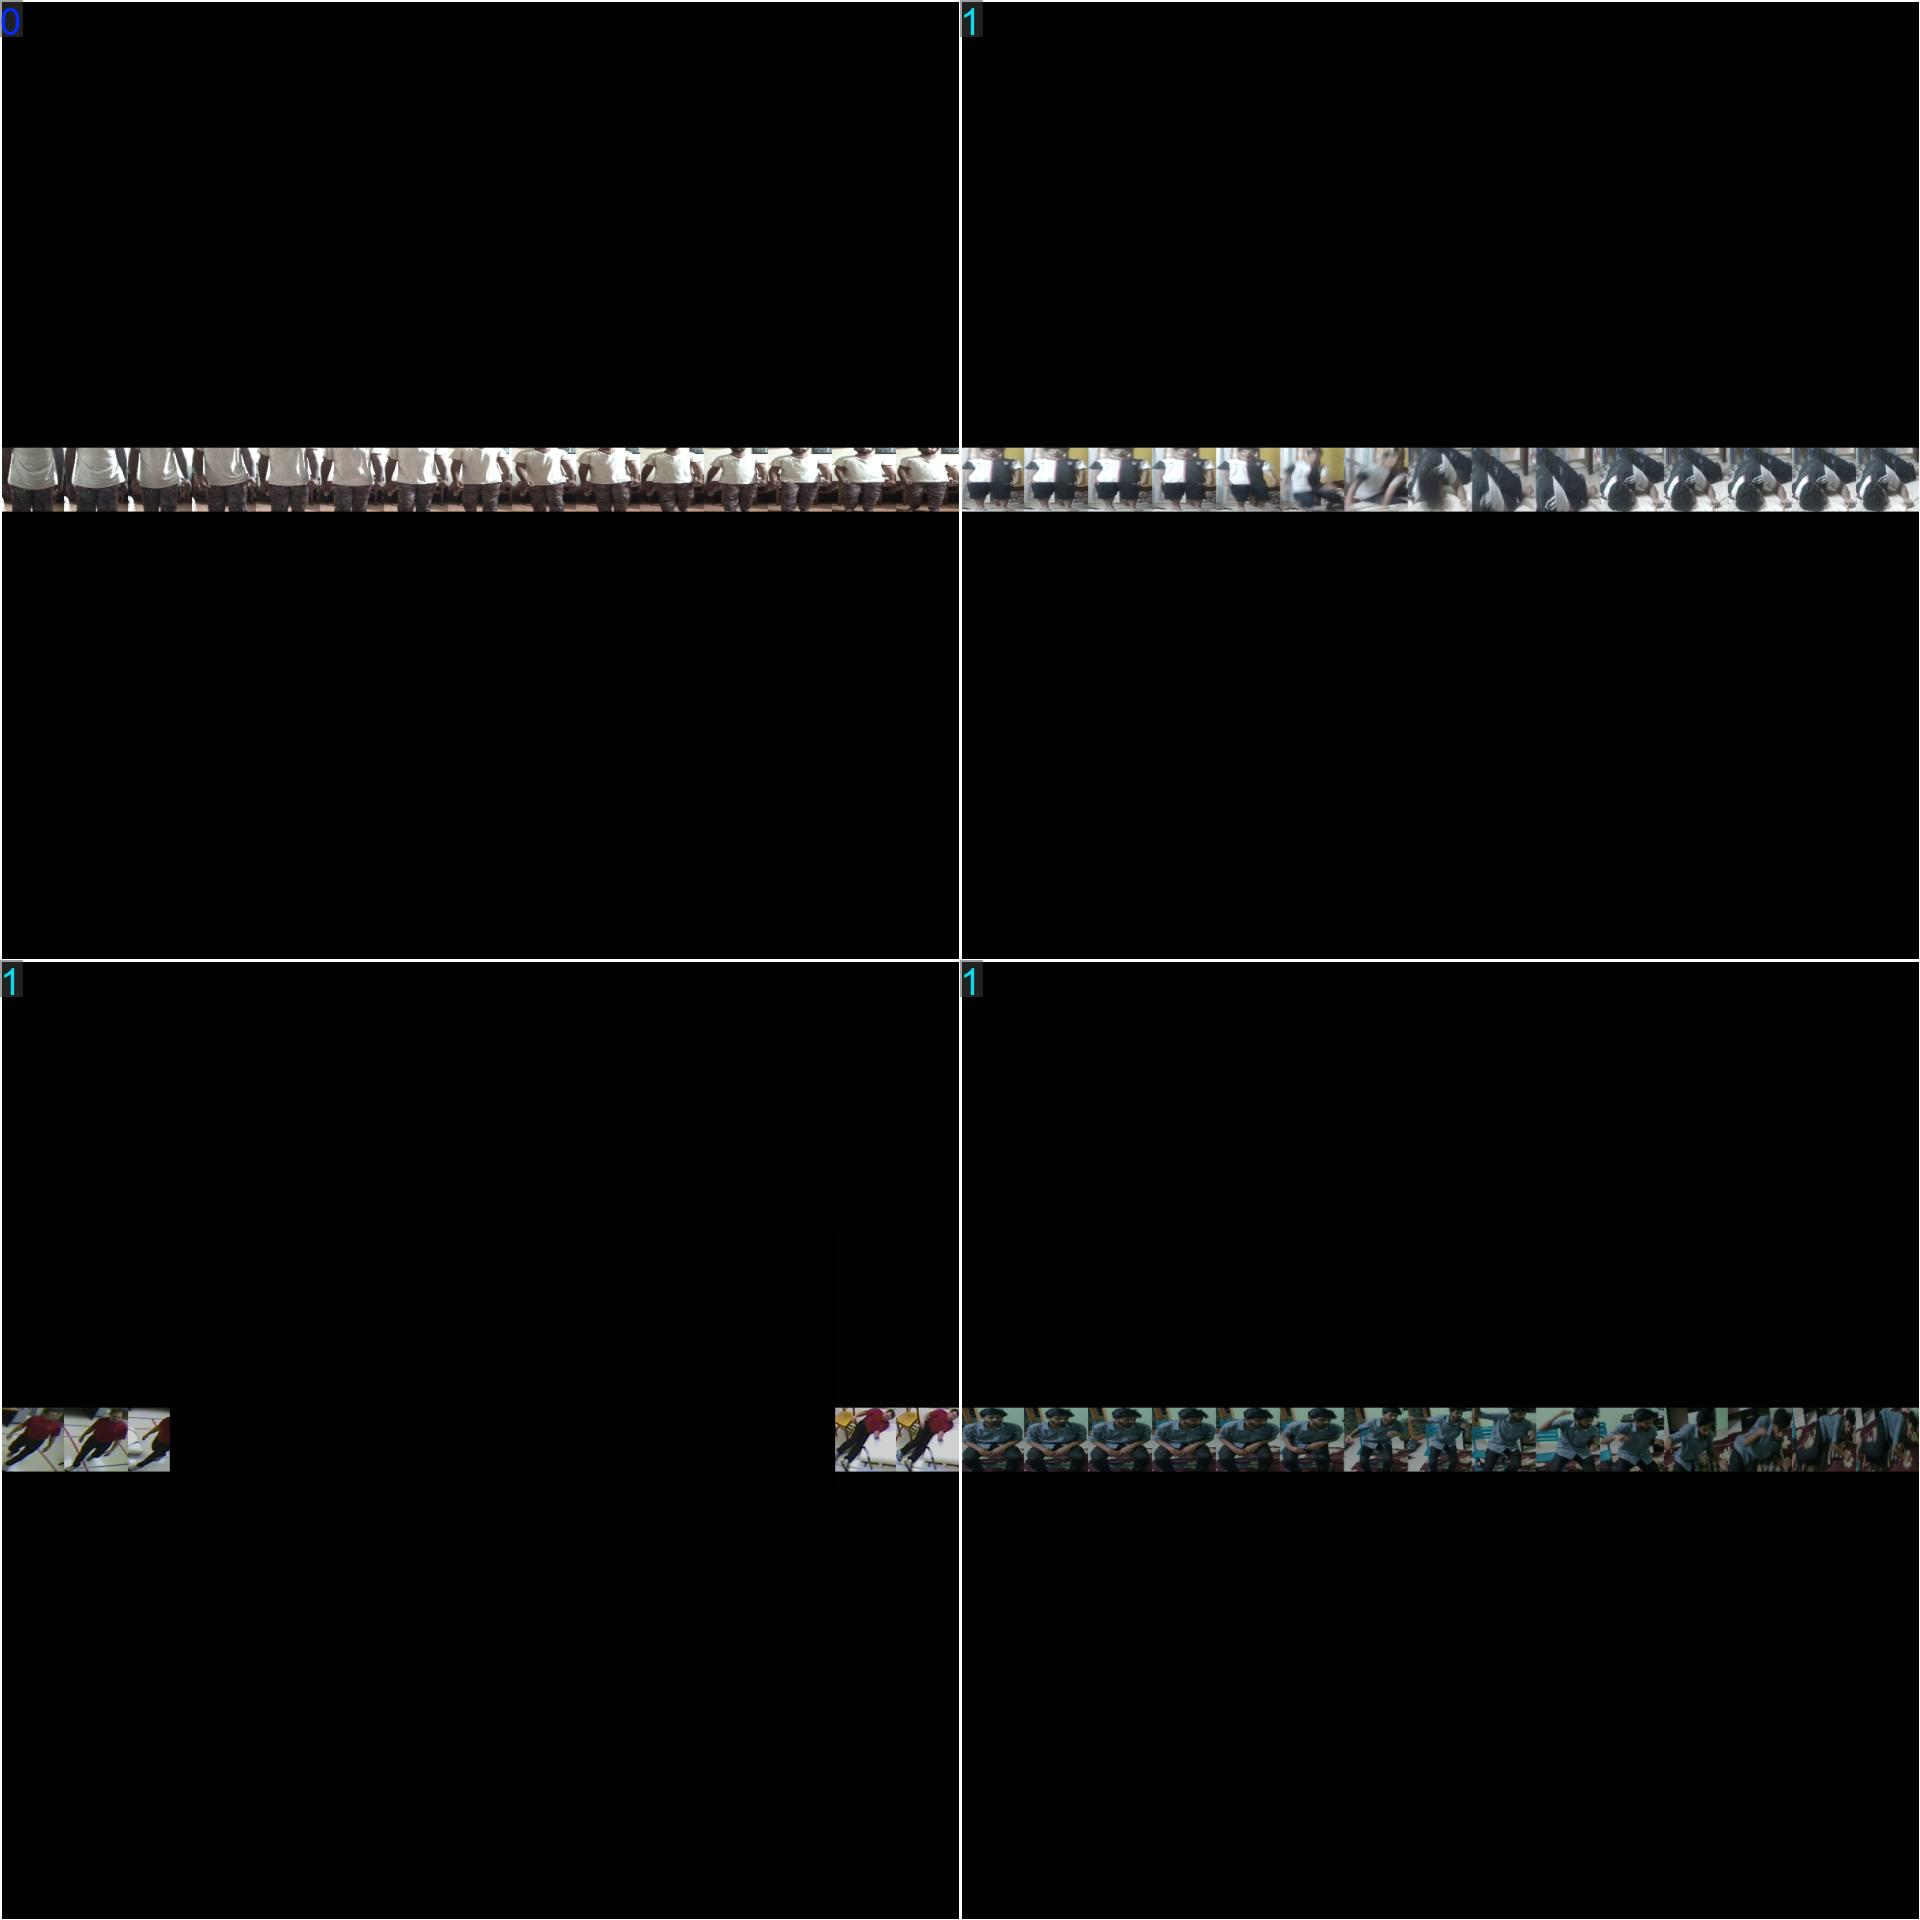
\includegraphics[width=\linewidth]{./imgs/t2-train_batch.jpg}
        \caption{Amostra de batch.}

    \end{subfigure}
    \hspace{0.05\linewidth}
    \begin{subfigure}[b]{0.45\linewidth}
        \centering
        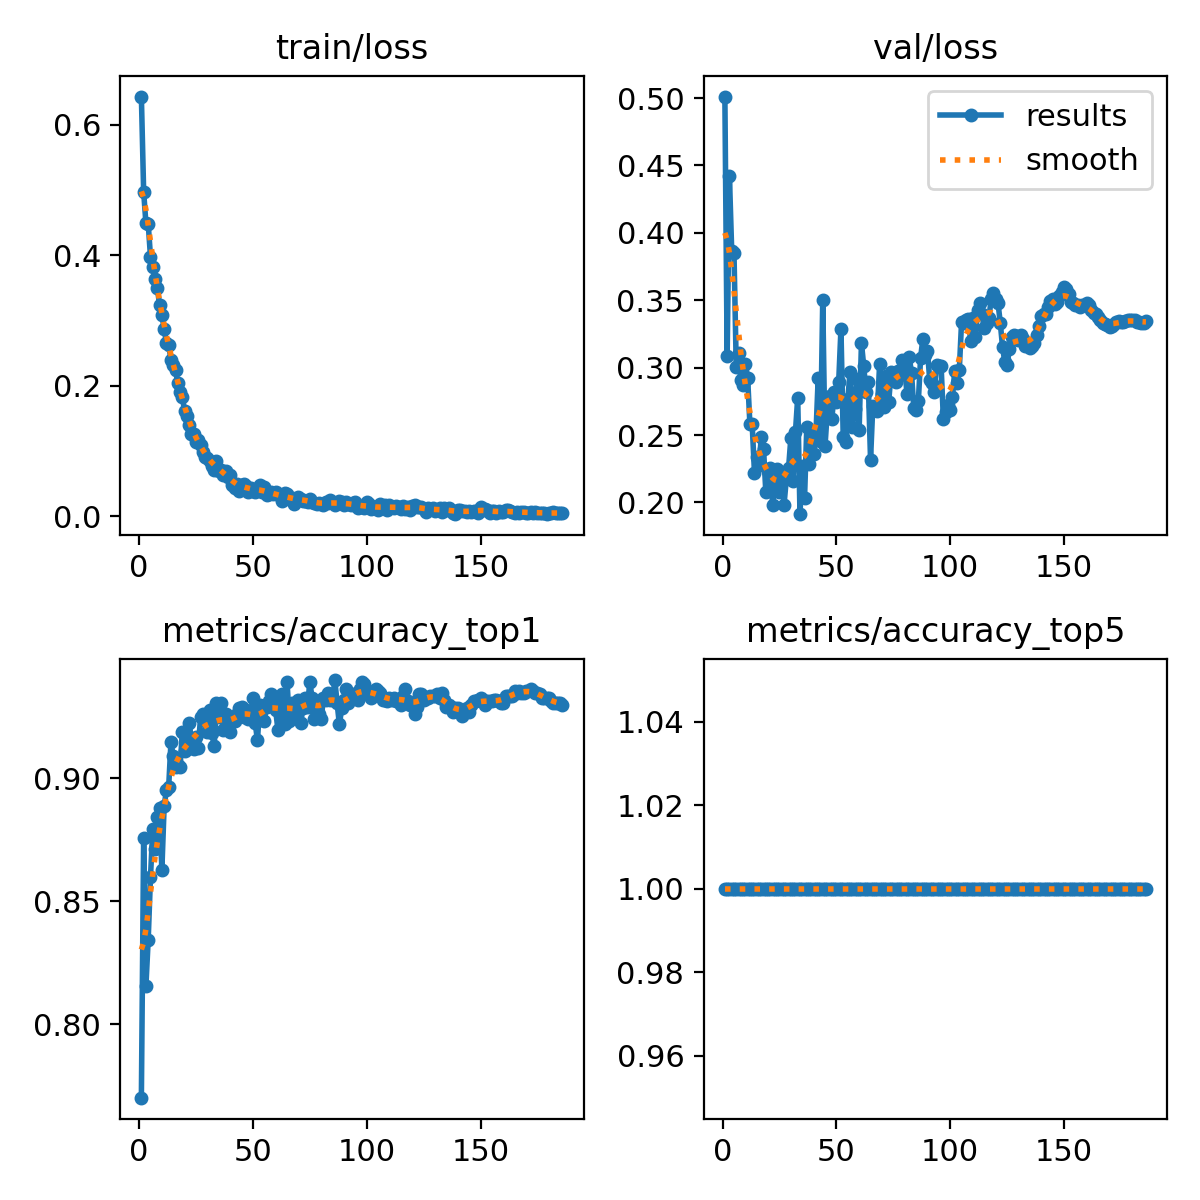
\includegraphics[width=\linewidth]{./imgs/t2-results.png}
        \caption{Métricas de desempenho.}

    \end{subfigure}
    \caption{Treinamento 2: amostra de batch e métricas de desempenho.}
    \label{fig:t2-1}
\end{figure}

Sobre o comportamento das métricas de desempenho, verifica-se que as suas evoluções também apresentaram um padrão esperado (\textbf{Figura \ref{fig:t2-1}}). A evolução da função de perda para os dados de validação apresentou um comportamento mais dinâmico. Ela convergiu mais rápido para uma condição de valor mínino e depois começou gradualmente a divergir desse valor. Uma justificativa desse comportamento pode ser encontrada pela remoção da aumentação de dados de rotação. Sem essa aumentação de dados, as imagens de entrada utilizadas no treinamento apresentaram um comportamento mais prevesível que facilitou o ajuste de pesos da rede durante o treinamento.


\begin{figure}[H]
    \centering
    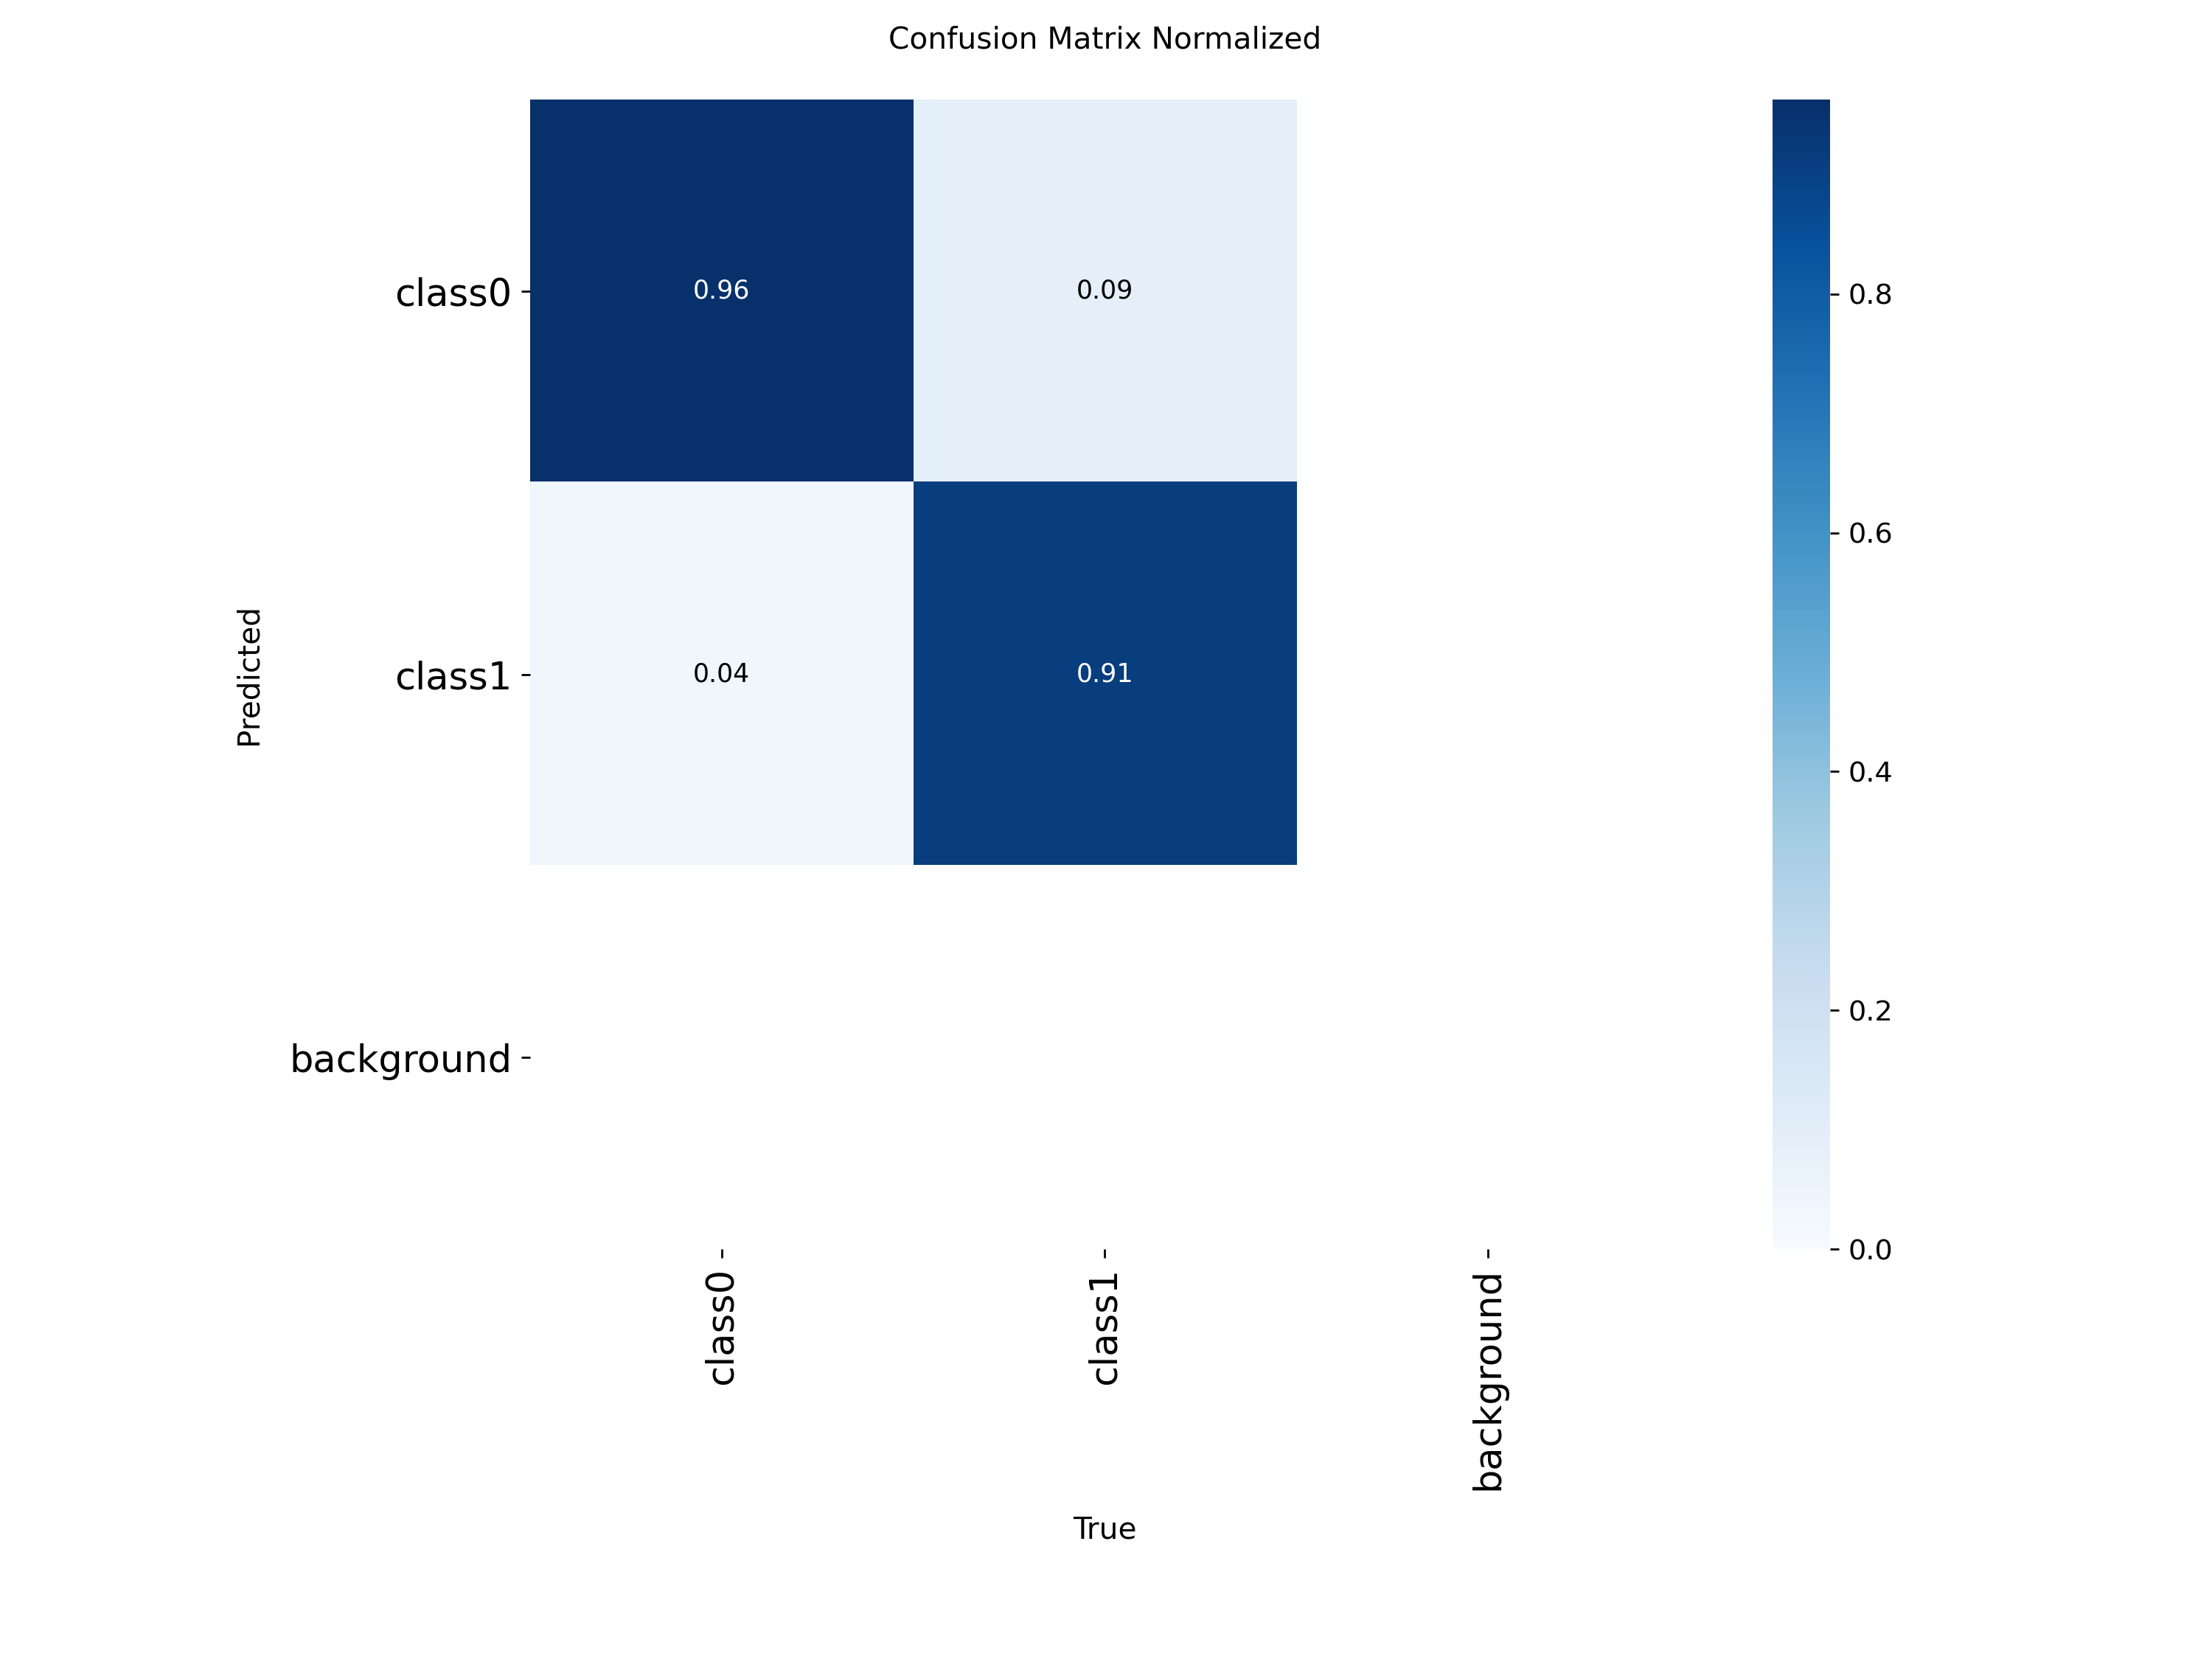
\includegraphics[width=0.80\linewidth]{./imgs/t2-confusion_matrix_normalized.png}
    \caption{Treinamento 2: matriz de confusão normalizada.}
    \label{fig:t2-2}
\end{figure}

Neste treinamento, a matriz de confusão também apresentou bons resultados (\textbf{Figura \ref{fig:t2-2}}).

\subsection{Treinamento 3}\label{sec:t3}
Neste treinamento, a composição das imagena foi realizada pela moldura matricial. A única aumentação de dados mantida foi a de recorte. A evolução das métricas de desempenho apresentaram comportamento esperado  (\textbf{Figura \ref{fig:t3-1}}).


\begin{figure}[H]
    \centering
    \begin{subfigure}[b]{0.45\linewidth}
        \centering
        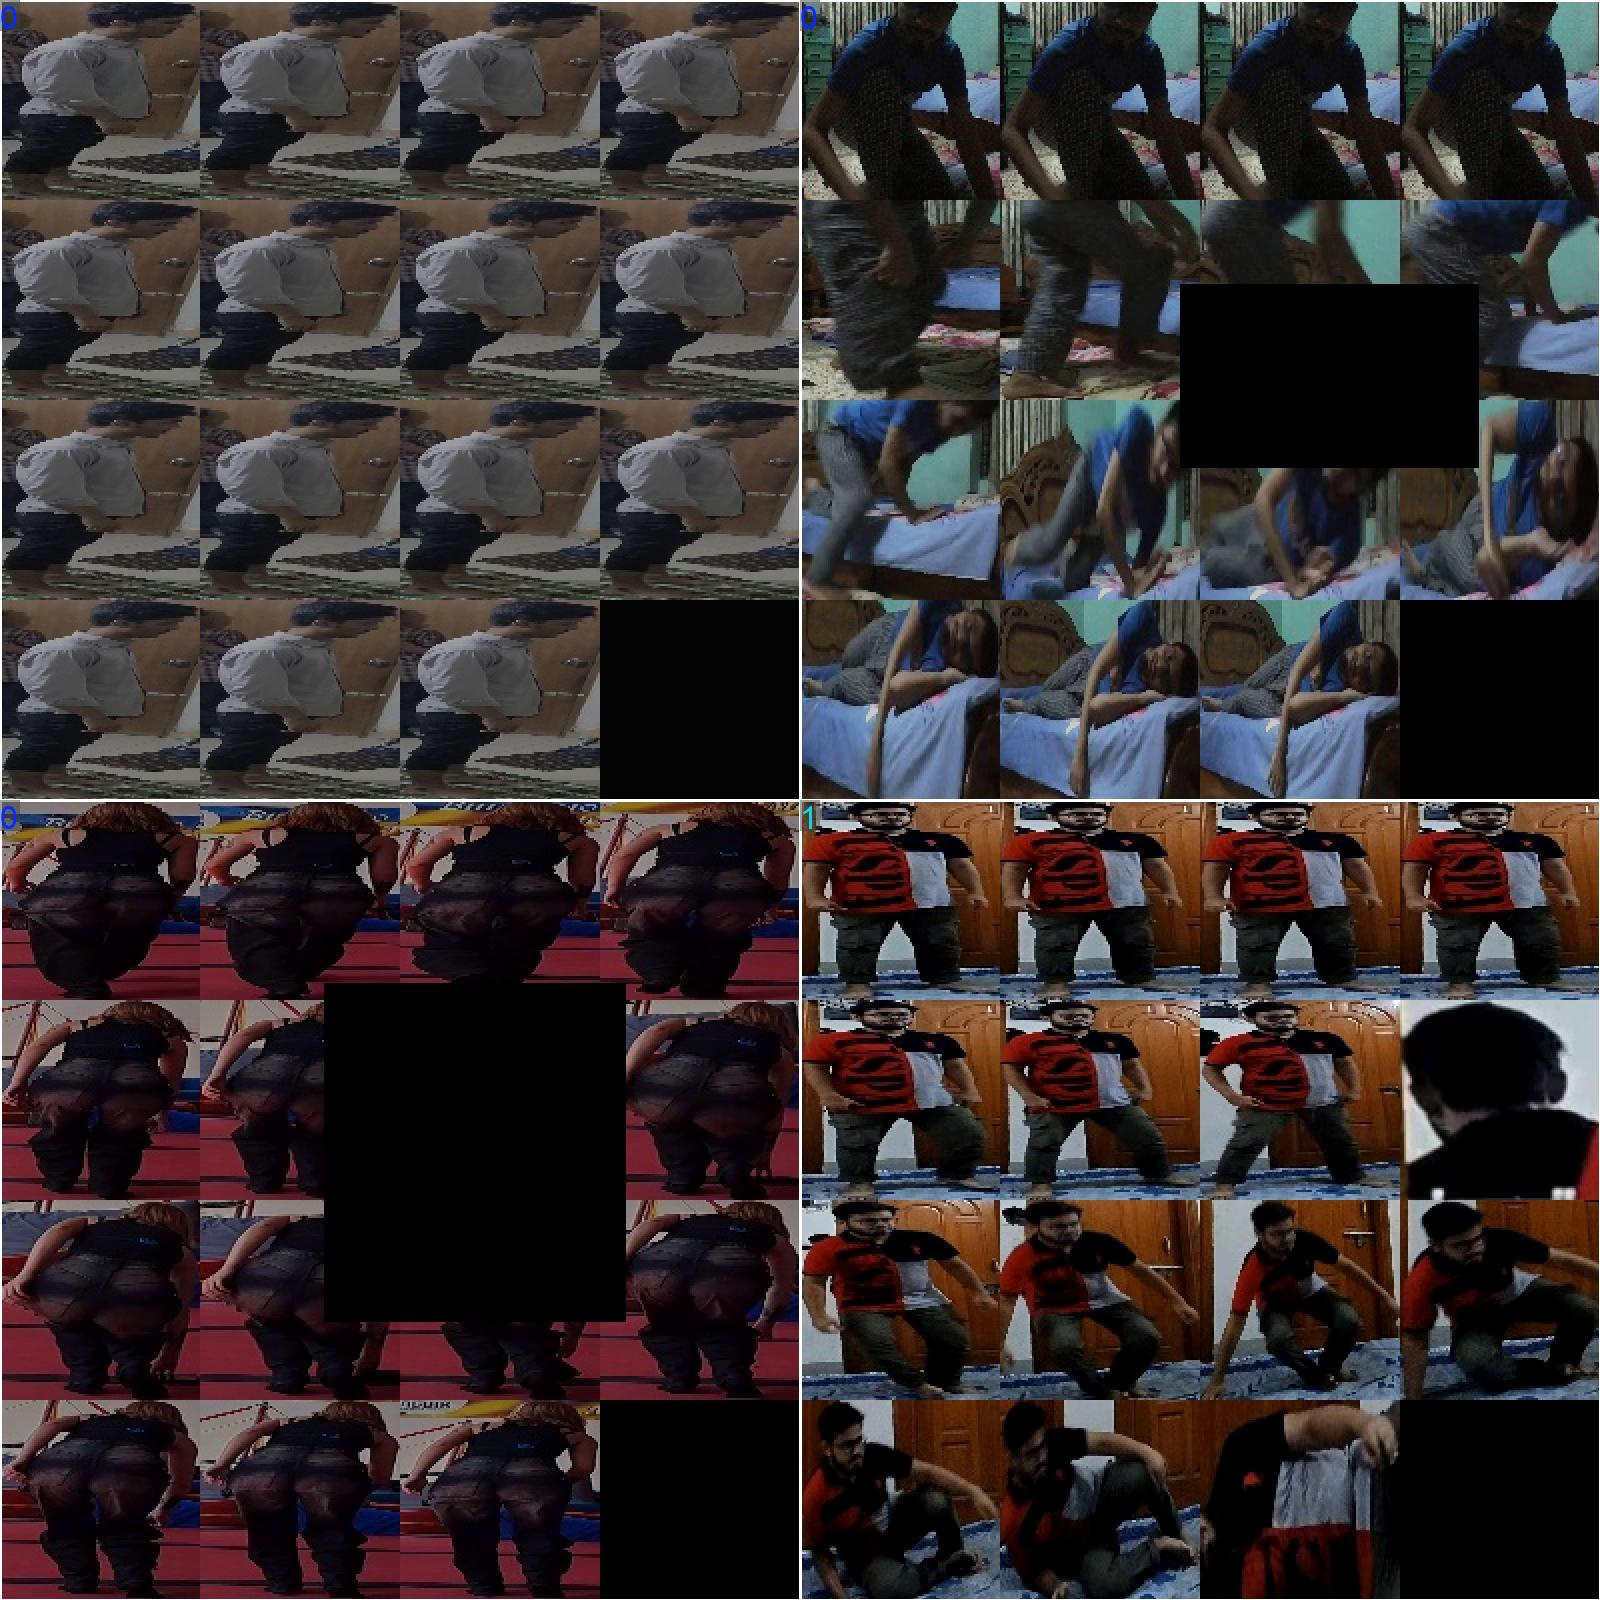
\includegraphics[width=\linewidth]{./imgs/t3-train_batch.jpg}
        \caption{Amostra de batch.}

    \end{subfigure}
    \hspace{0.05\linewidth}
    \begin{subfigure}[b]{0.45\linewidth}
        \centering
        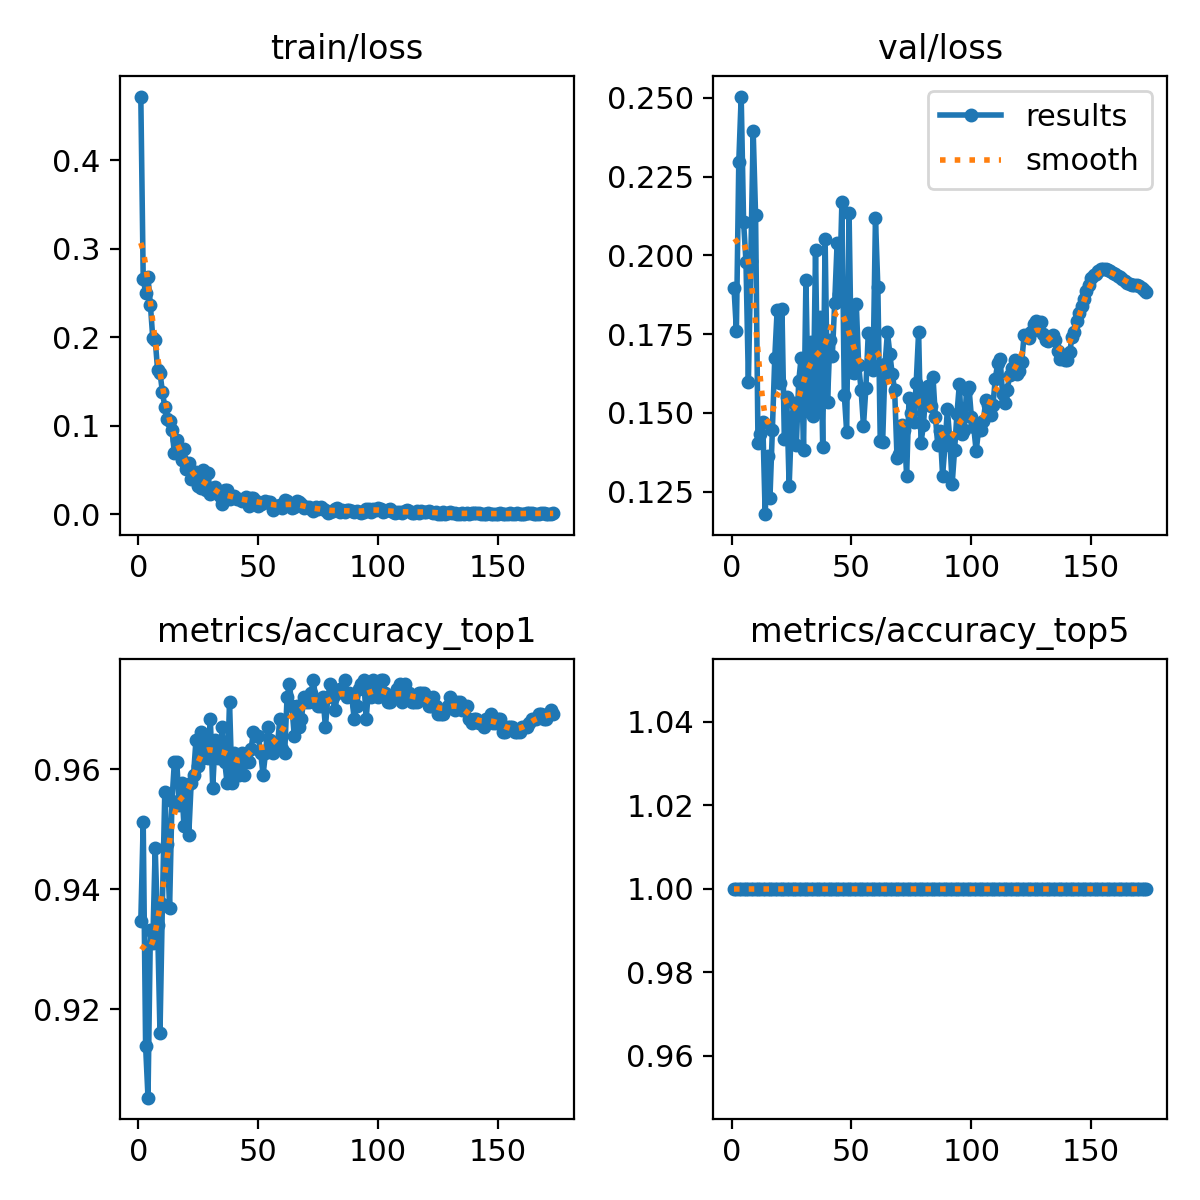
\includegraphics[width=\linewidth]{./imgs/t3-results.png}
        \caption{Métricas de desempenho.}

    \end{subfigure}
    \caption{Treinamento 3: amostra de batch e métricas de desempenho.}
    \label{fig:t3-1}
\end{figure}

Matriz de confusão normalizada mostra que o modelo está sendo capaz de aprender os padrões dentro da cobertura que as bases de dados estão fornecendo (\textbf{Figura \ref{fig:t3-2}}).

\begin{figure}[H]
    \centering
    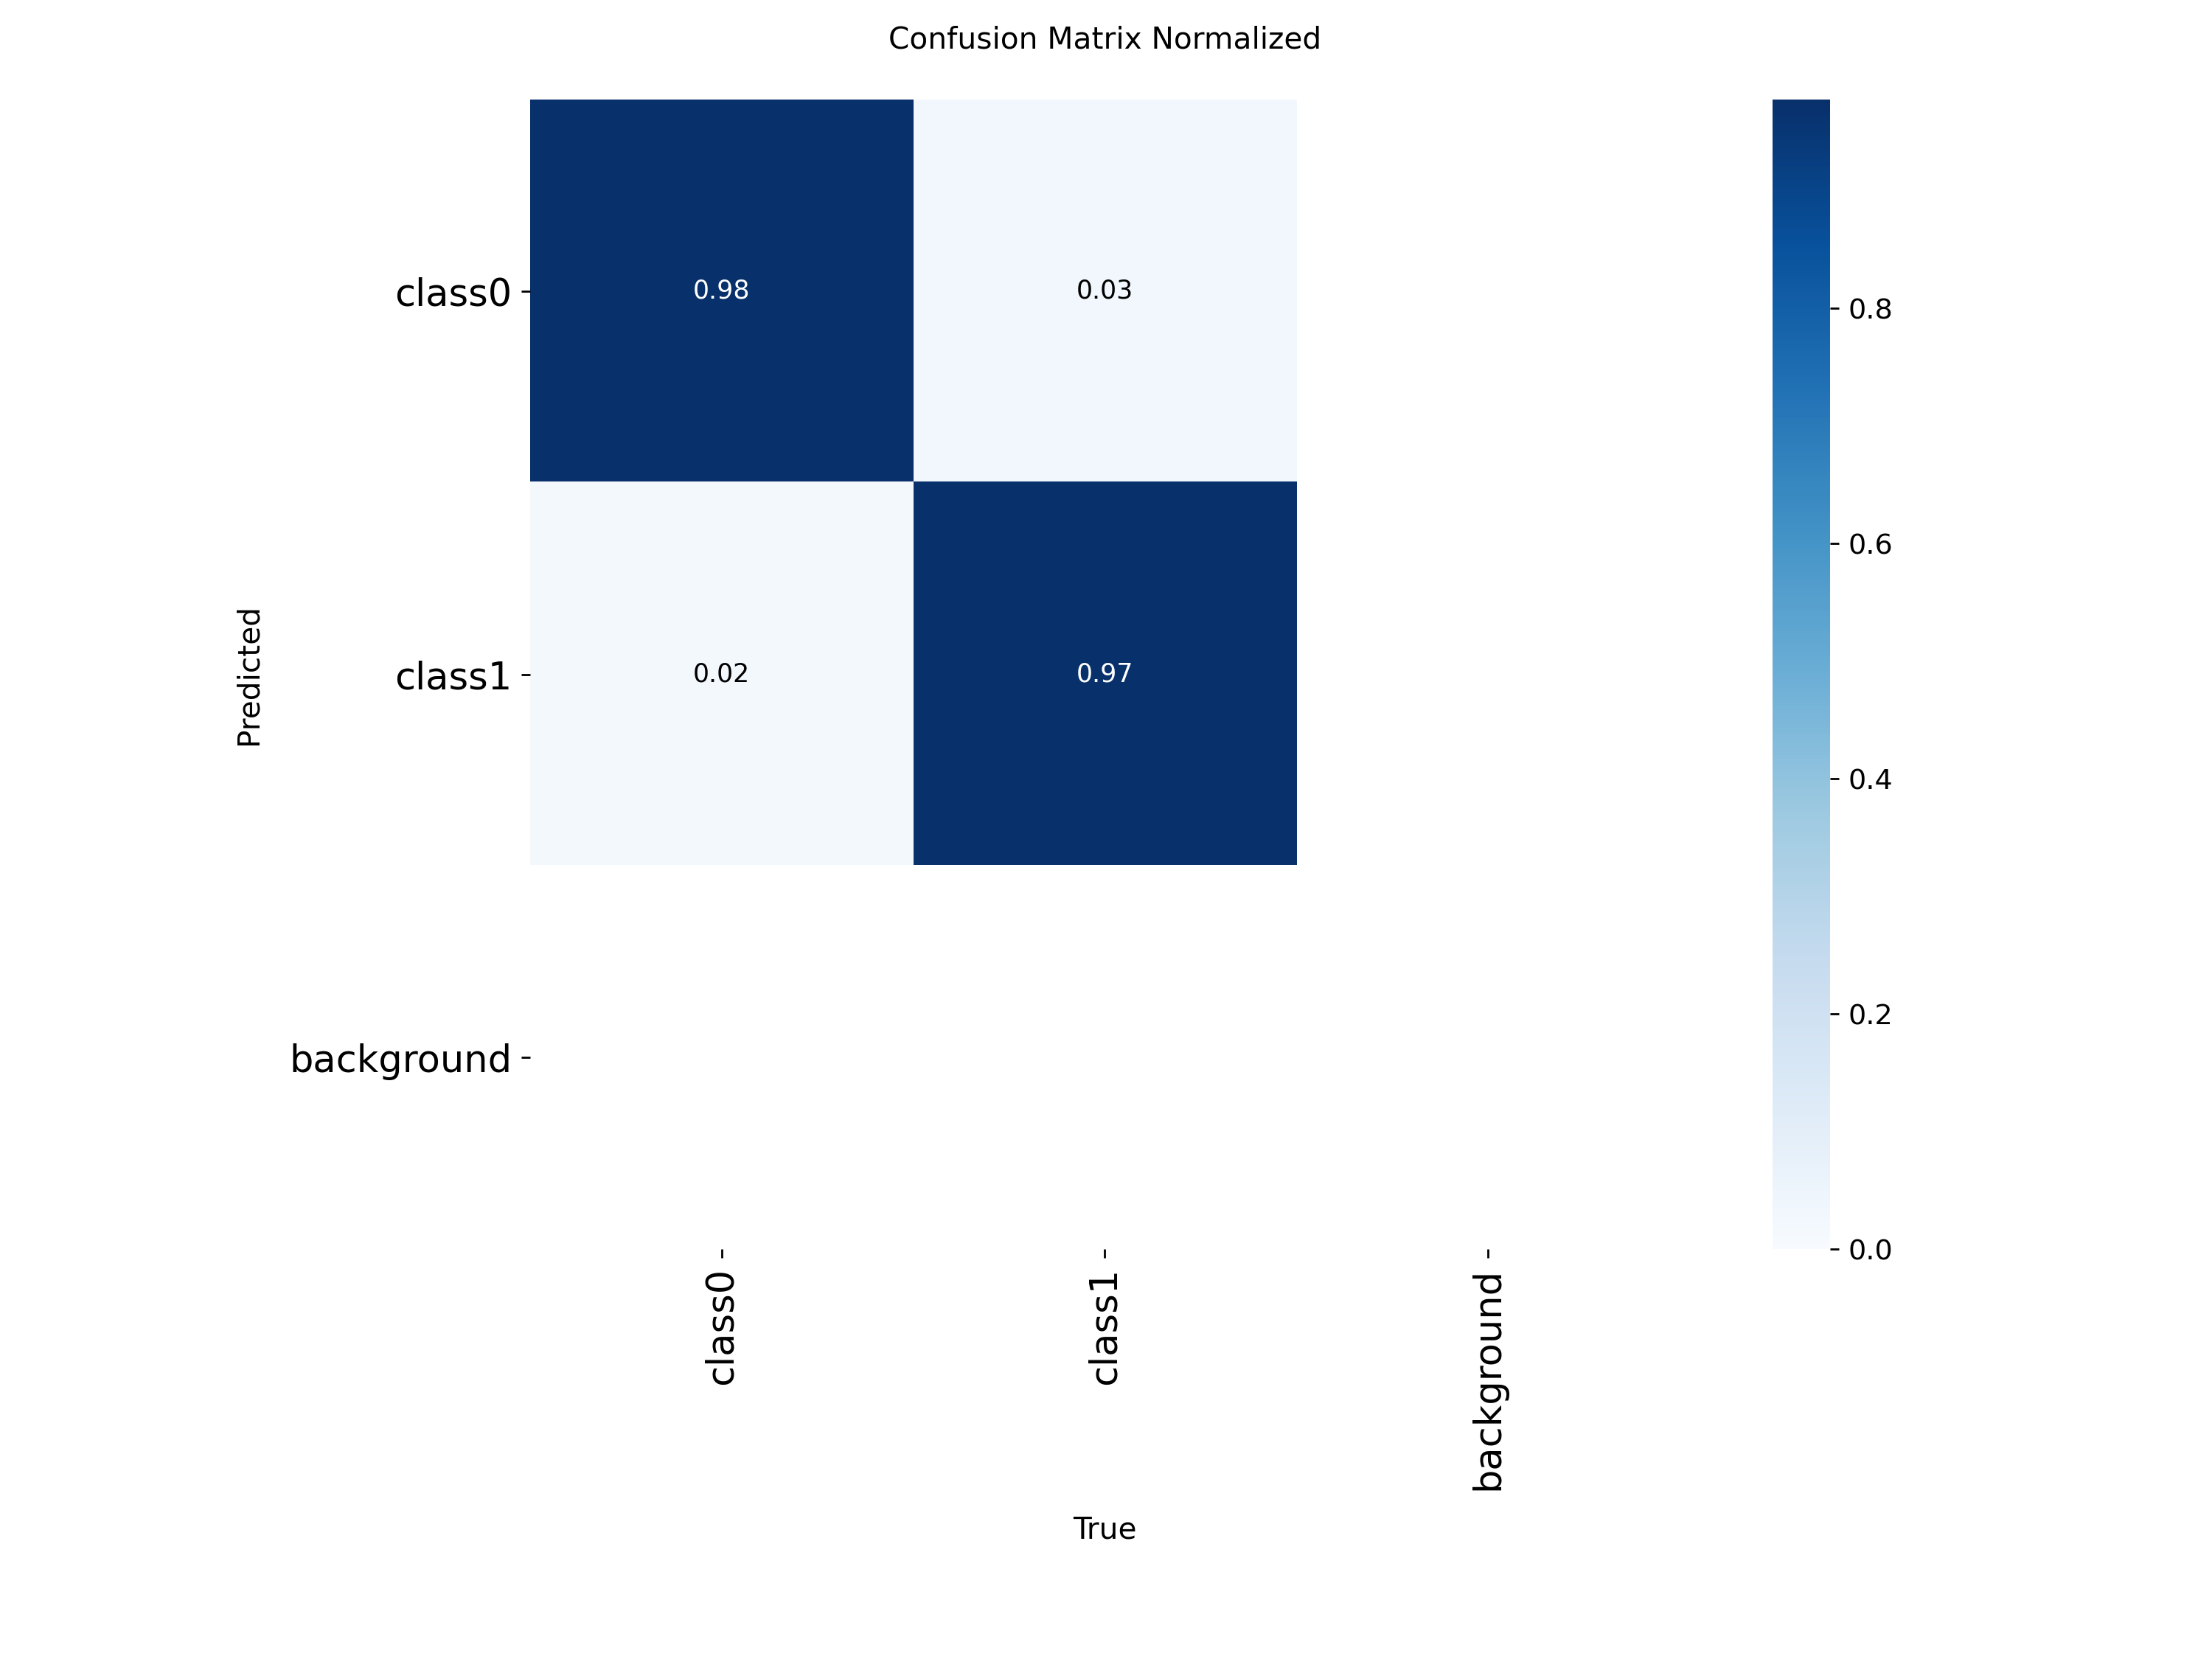
\includegraphics[width=0.80\linewidth]{./imgs/t3-confusion_matrix_normalized.png}
    \caption{Treinamento 3: matriz de confusão normalizada.}
    \label{fig:t3-2}
\end{figure}


\subsection{Treinamento 4}\label{sec:t4}
Devido às boas métricas de desempenho das matrizes de confusão apresentadas pelos modelos treinados anteriormente (treinamentos 1, 2 e 3) de maneira independente das estratégias de aumentação de dados aplicadas, uma desconfiança sobre uma possível condição de vazamento de dados se estabeleceu. Essa desconfiânça foi confirmada pela análise cuidadosa dos nomes dos vídeos geradores das imagens de treinamento e da estratégia de divisão entre dados de treinamento e dados de validação. Os dados \textit{Fall Video Dataset} apresentam uma nomeação com uso de prefixos e marcadores incosistente de modo que a divisão desses dados a partir de uma separação por nomes não era efetiva em evitar que dados de mesma origem ou até mesmo das mesmas pessoas fossem parar tanto nos grupos de dados de treino e de dados de validação. Neste momento, para contornar esse problema, uma separação rigosa e manual foi realizada sobre os dados de modo a garantir que vídeos de mesma origem não fossem distribuídos entre conjuntos de treinamento e de validação.



\begin{figure}[H]
    \centering
    \begin{subfigure}[b]{0.45\linewidth}
        \centering
        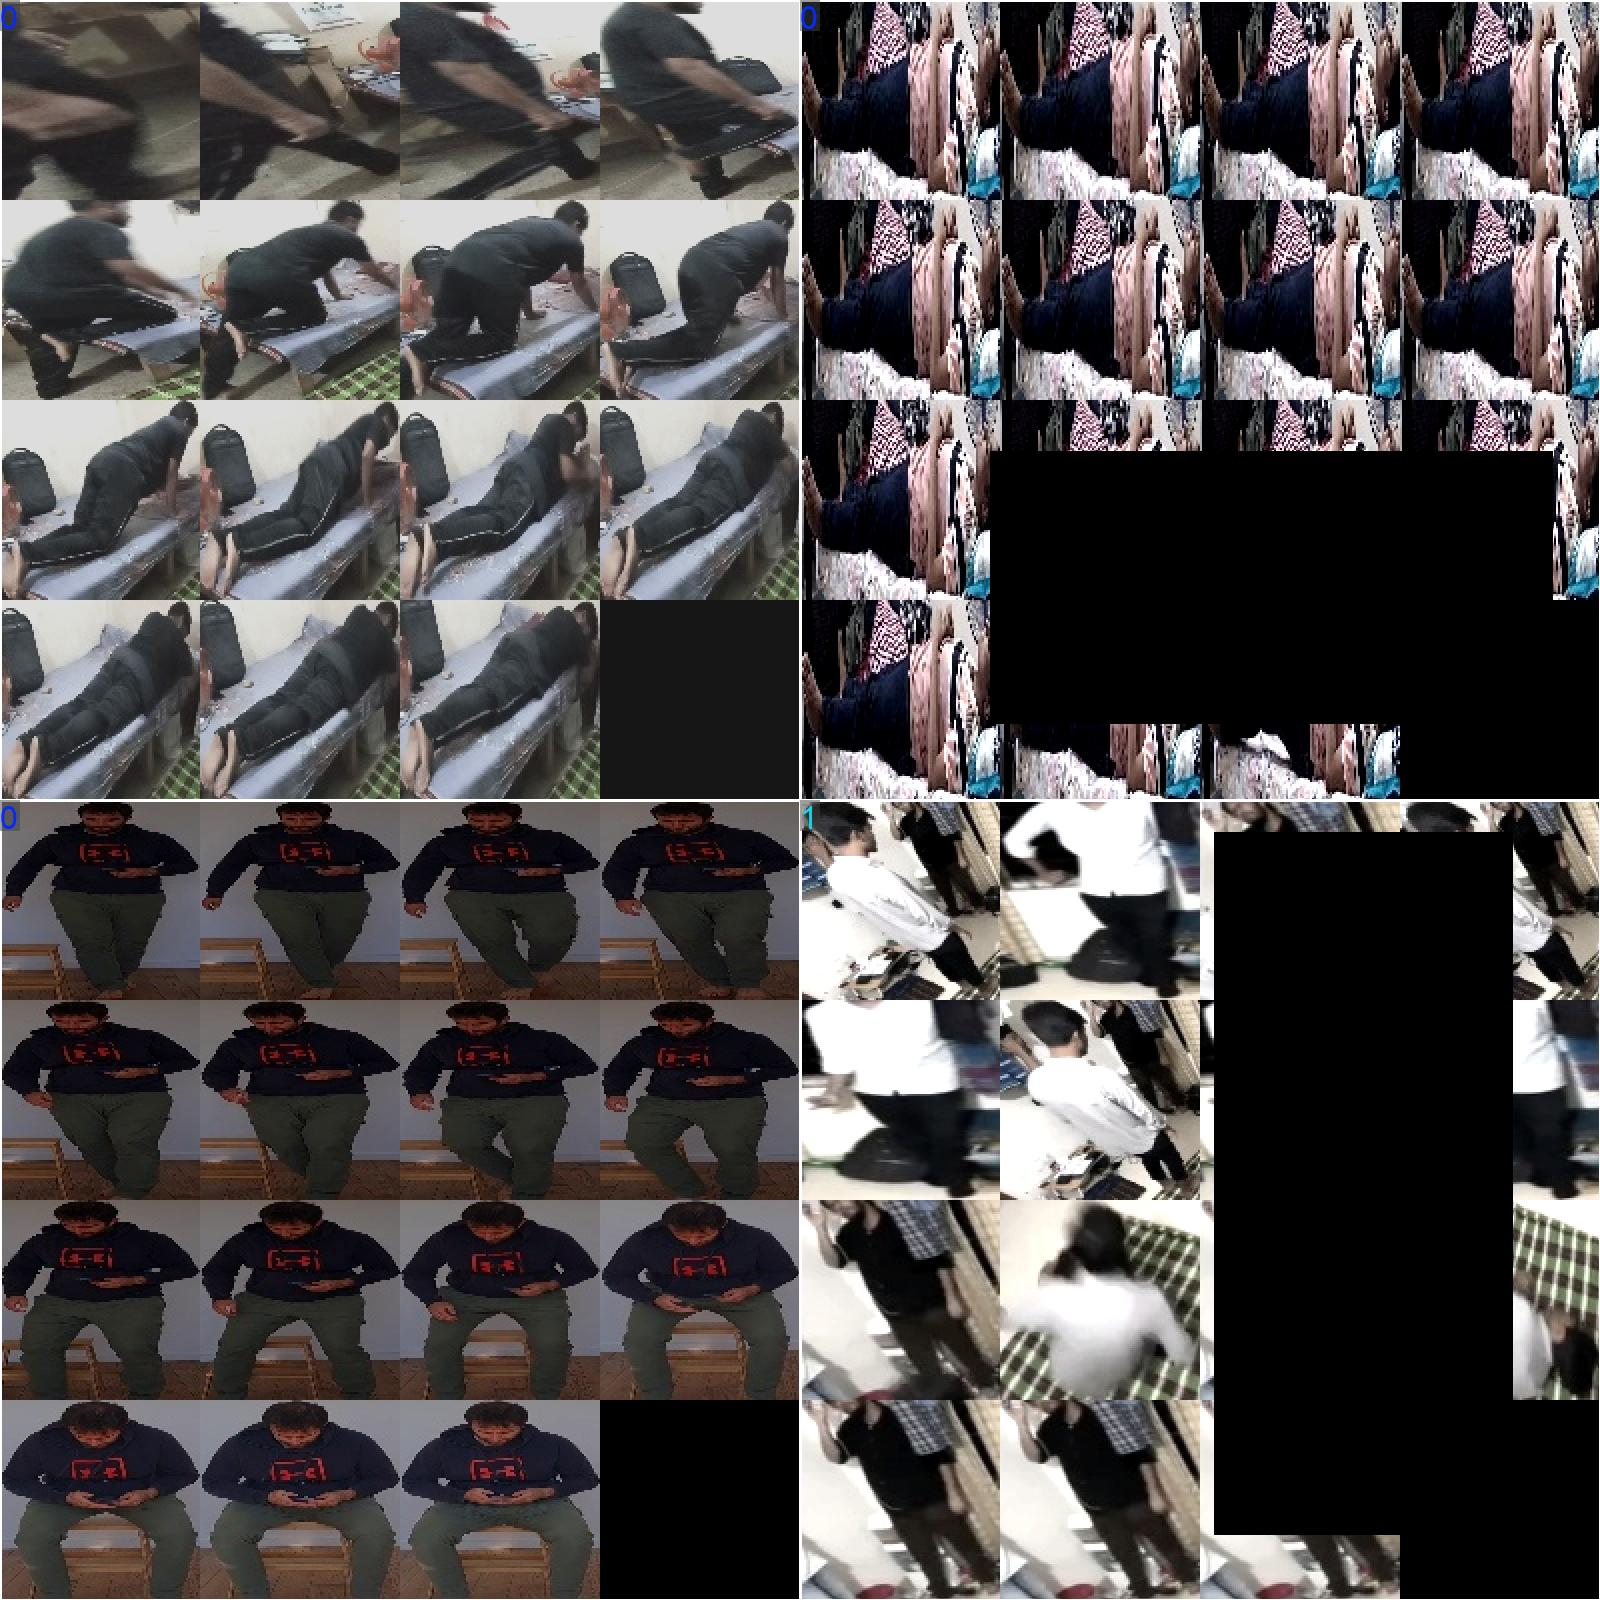
\includegraphics[width=\linewidth]{./imgs/t4-train_batch.jpg}
        \caption{Amostra de batch.}

    \end{subfigure}
    \hspace{0.05\linewidth}
    \begin{subfigure}[b]{0.45\linewidth}
        \centering
        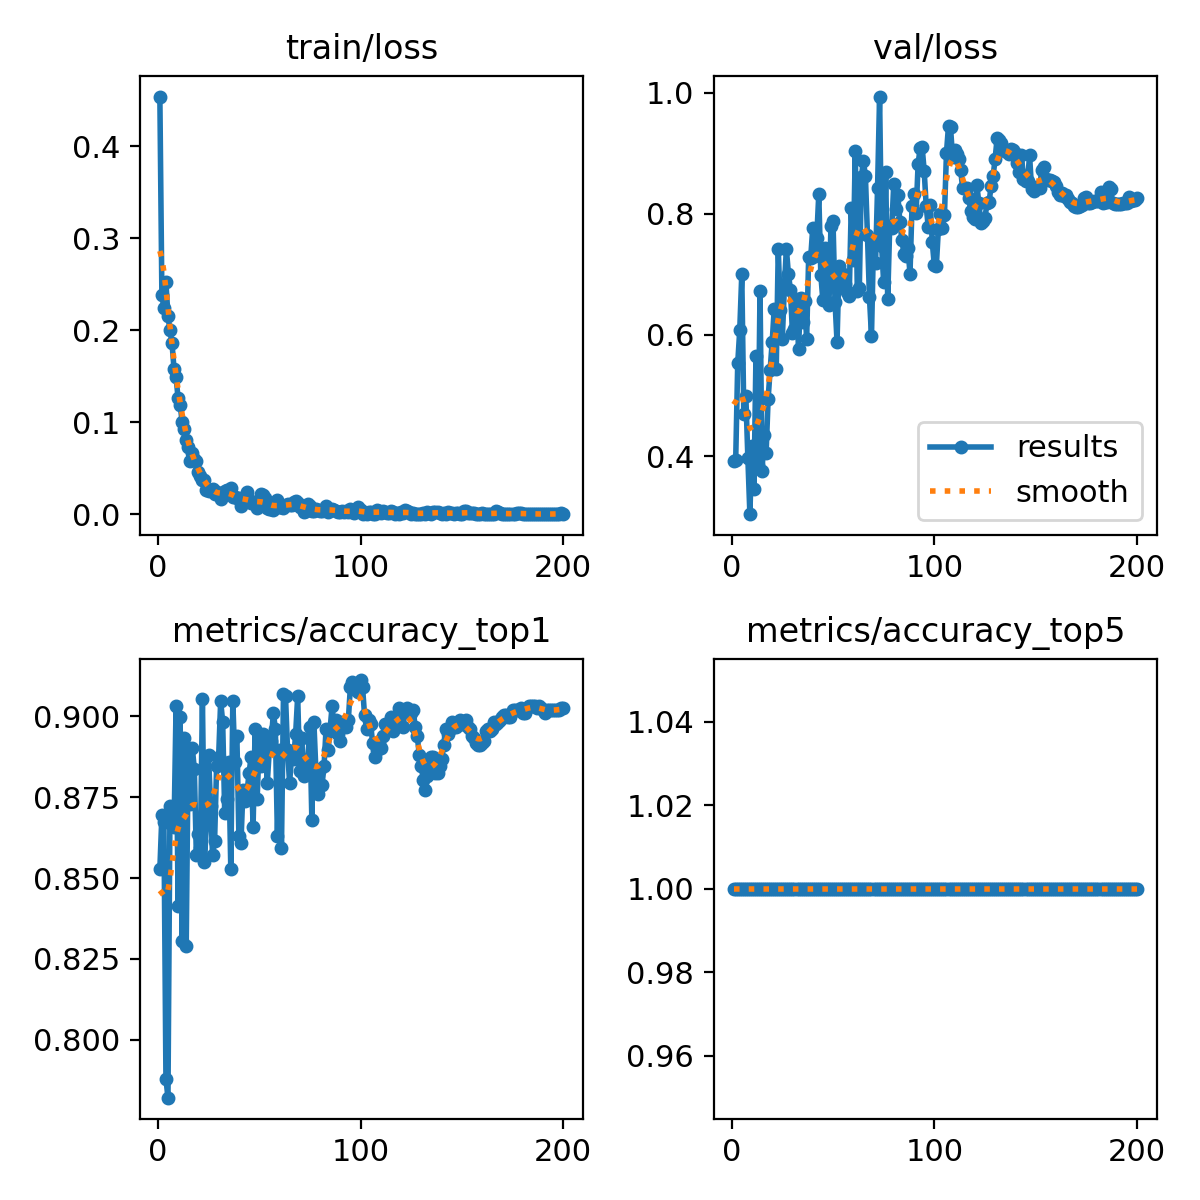
\includegraphics[width=\linewidth]{./imgs/t4-results.png}
        \caption{Métricas de desempenho.}

    \end{subfigure}
    \caption{Treinamento 4: amostra de batch e métricas de desempenho.}
    \label{fig:t4-1}
\end{figure}

As métricas de desempenho durante o treinamento se comportaram da maneira esperada (\textbf{Figura \ref{fig:t4-1}}). Já as métricas de qualidade do modelo treinado a partir da matriz de confusão normalizada mostram um modelo com desempenho mais modesto (\textbf{Figura \ref{fig:t4-2}}). 

\begin{figure}[H]
    \centering
    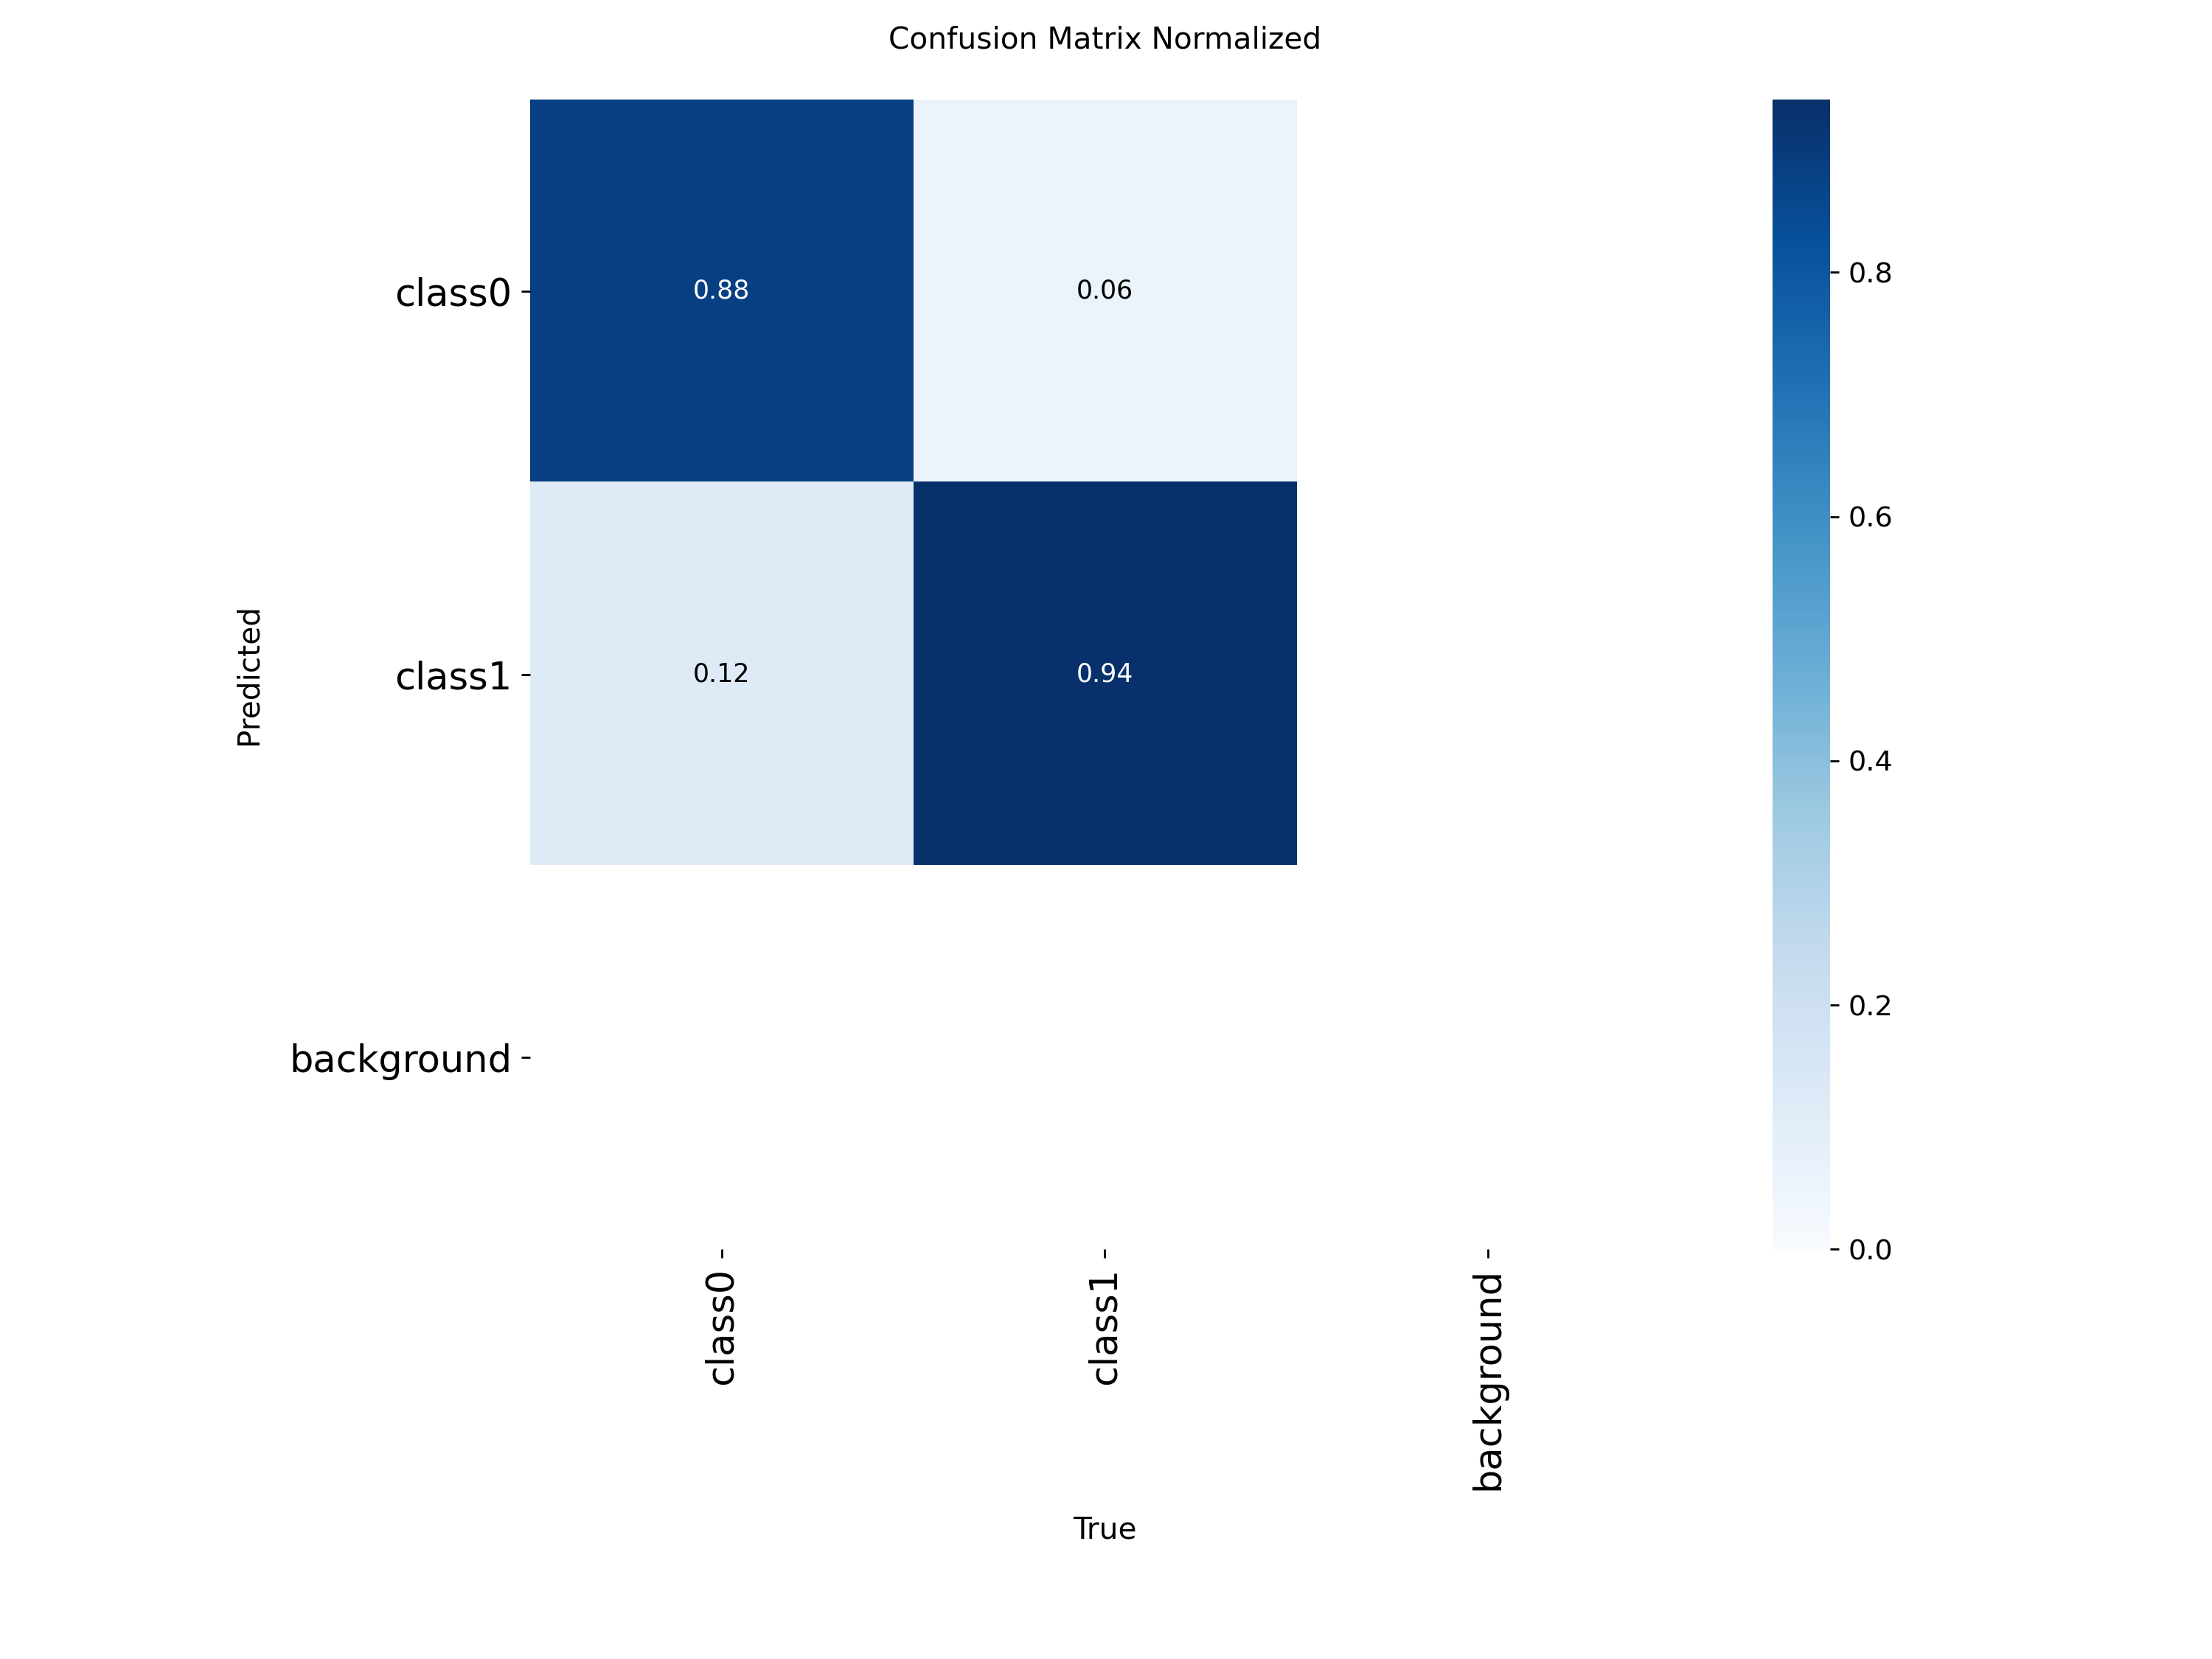
\includegraphics[width=0.80\linewidth]{./imgs/t4-confusion_matrix_normalized.png}
    \caption{Treinamento 4: matriz de confusão normalizada.}
    \label{fig:t4-2}
\end{figure}


\subsection{Treinamento 5}\label{sec:t5}
No treinamento 5 foi aplicado uma versão diferente da aumentação de dados de rotação. A rotação não foi aplicada na imagem final de modo a rodar todo o conteúdo da imagem. Neste momento, a rotação foi aplicada individualmente nas imagens menores. Os ângulos de rotação utilizados foram -30, -15, 0, 15 e 30 graus (\textbf{Figura \ref{fig:t5-1}}). 


\begin{figure}[H]
    \centering
    \begin{subfigure}[b]{0.45\linewidth}
        \centering
        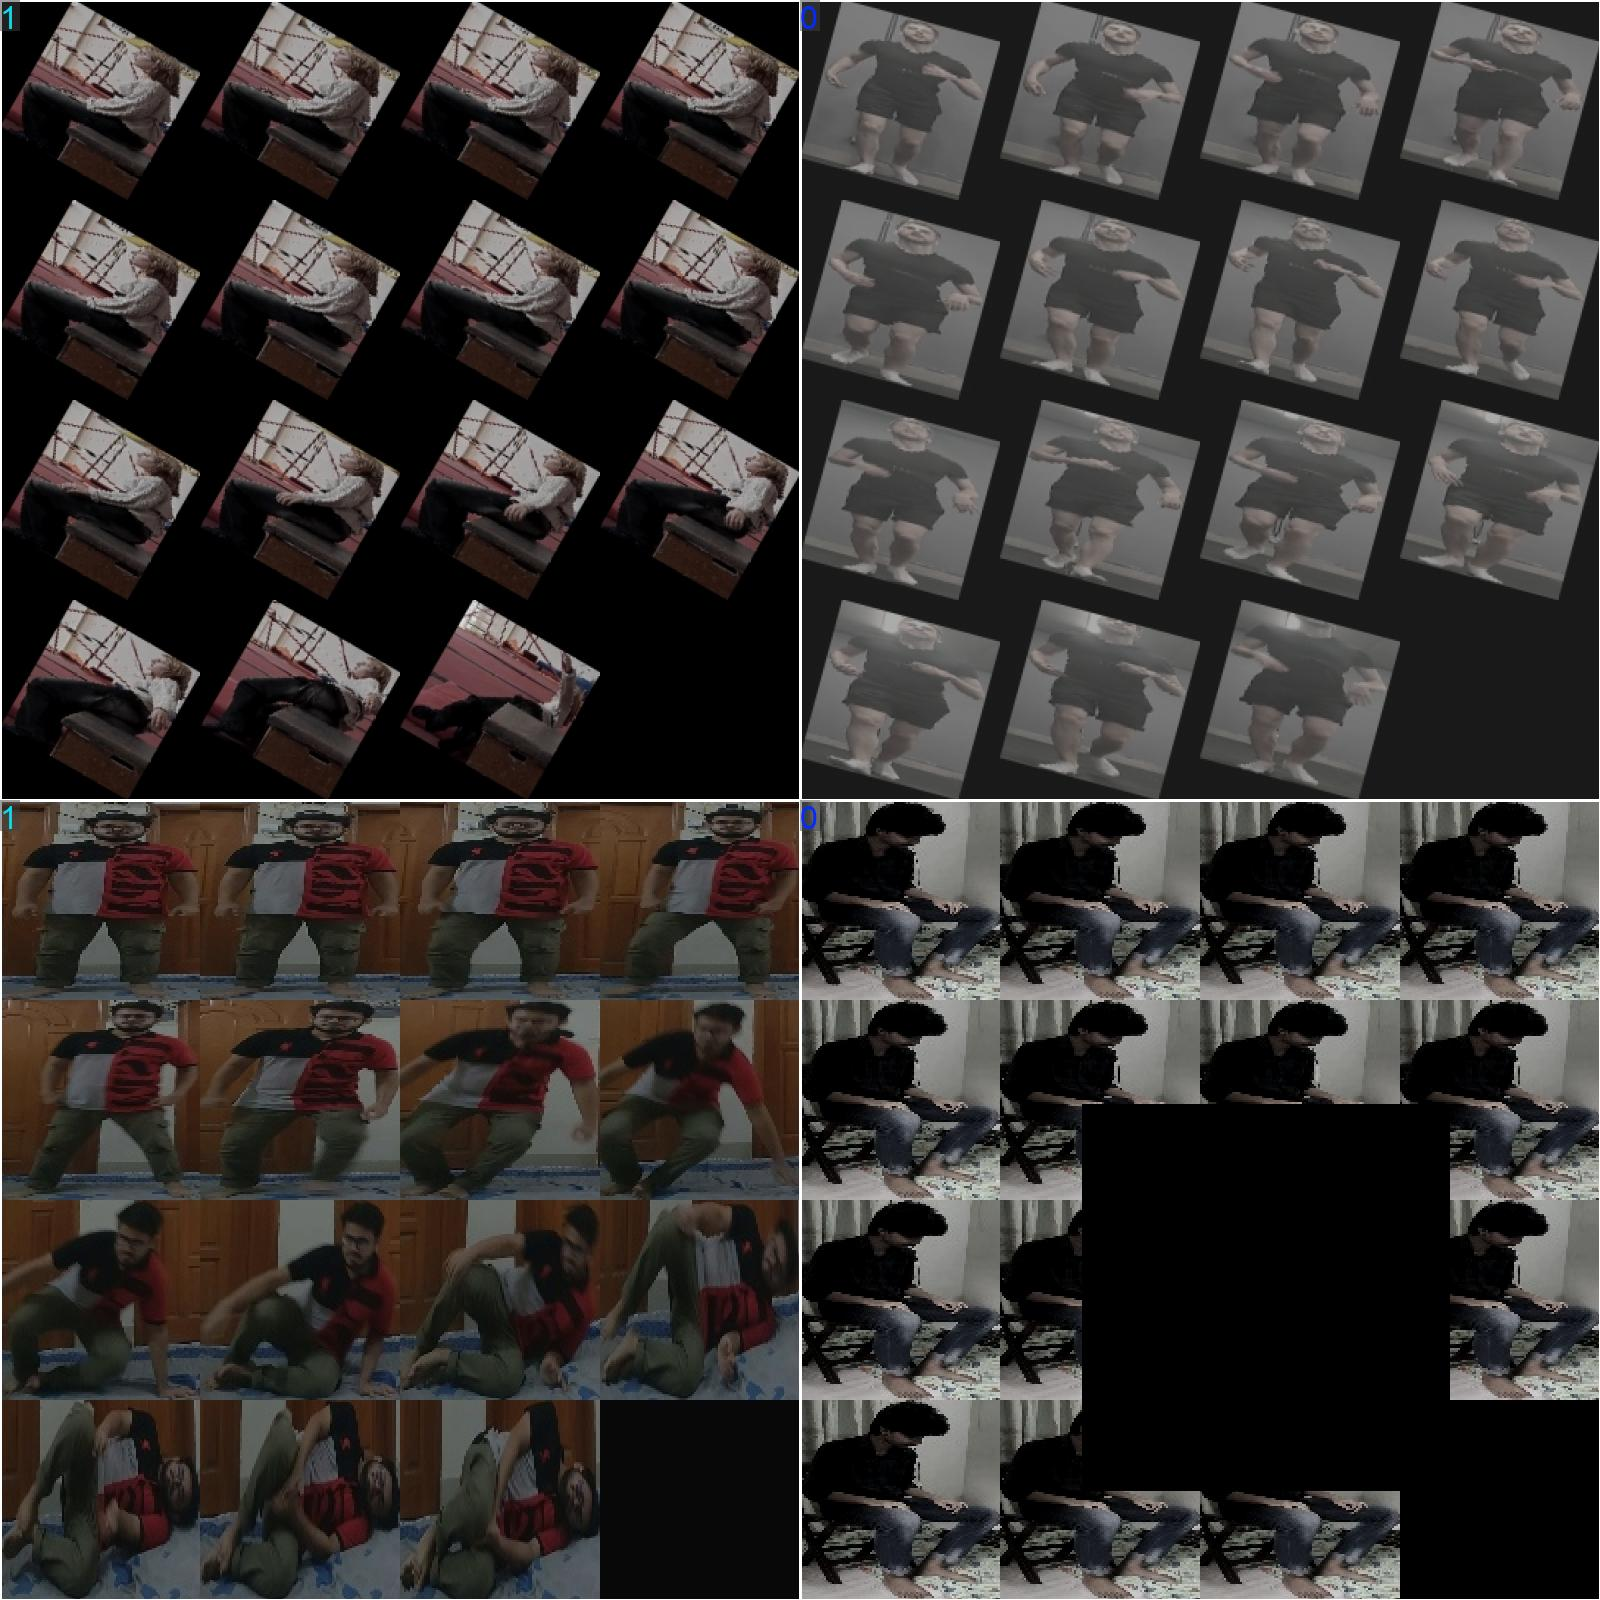
\includegraphics[width=\linewidth]{./imgs/t5-train_batch.jpg}
        \caption{Amostra de batch.}

    \end{subfigure}
    \hspace{0.05\linewidth}
    \begin{subfigure}[b]{0.45\linewidth}
        \centering
        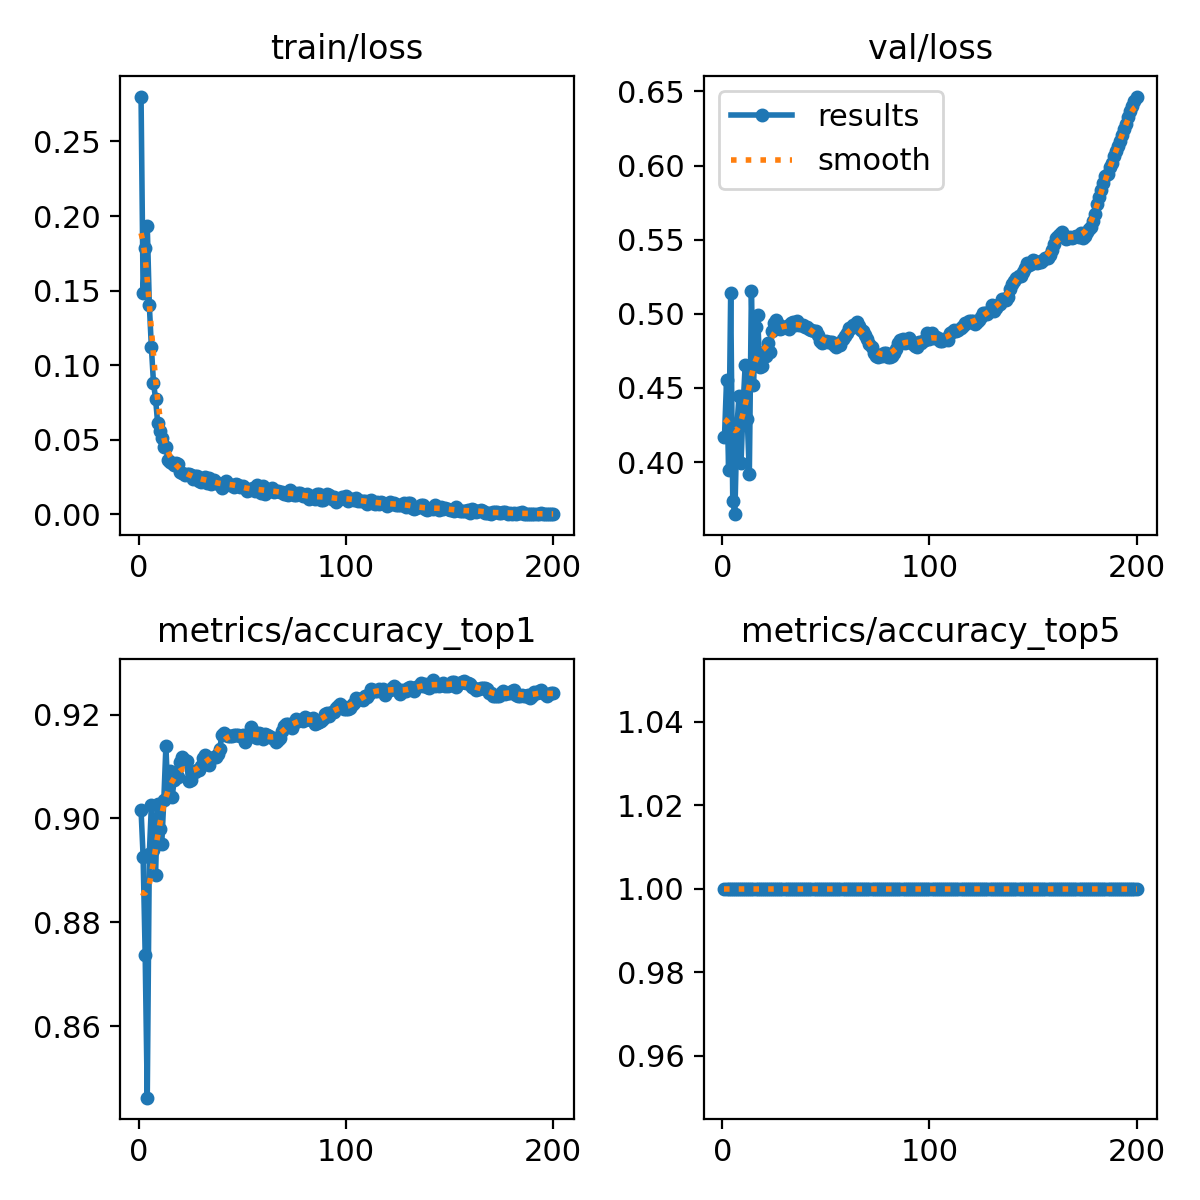
\includegraphics[width=\linewidth]{./imgs/t5-results.png}
        \caption{Métricas de desempenho.}

    \end{subfigure}
    \caption{Treinamento 5: amostra de batch e métricas de desempenho.}
    \label{fig:t5-1}
\end{figure}

As métricas de desempenho das funções de perda ao longo do treinamento se comportaram dentro de um padrão esperado (\textbf{Figura \ref{fig:t5-1}}). As métricas da matriz de confusão normalizada apresentaram uma ligeira melhora (\textbf{Figura \ref{fig:t5-2}}). 


\begin{figure}[H]
    \centering
    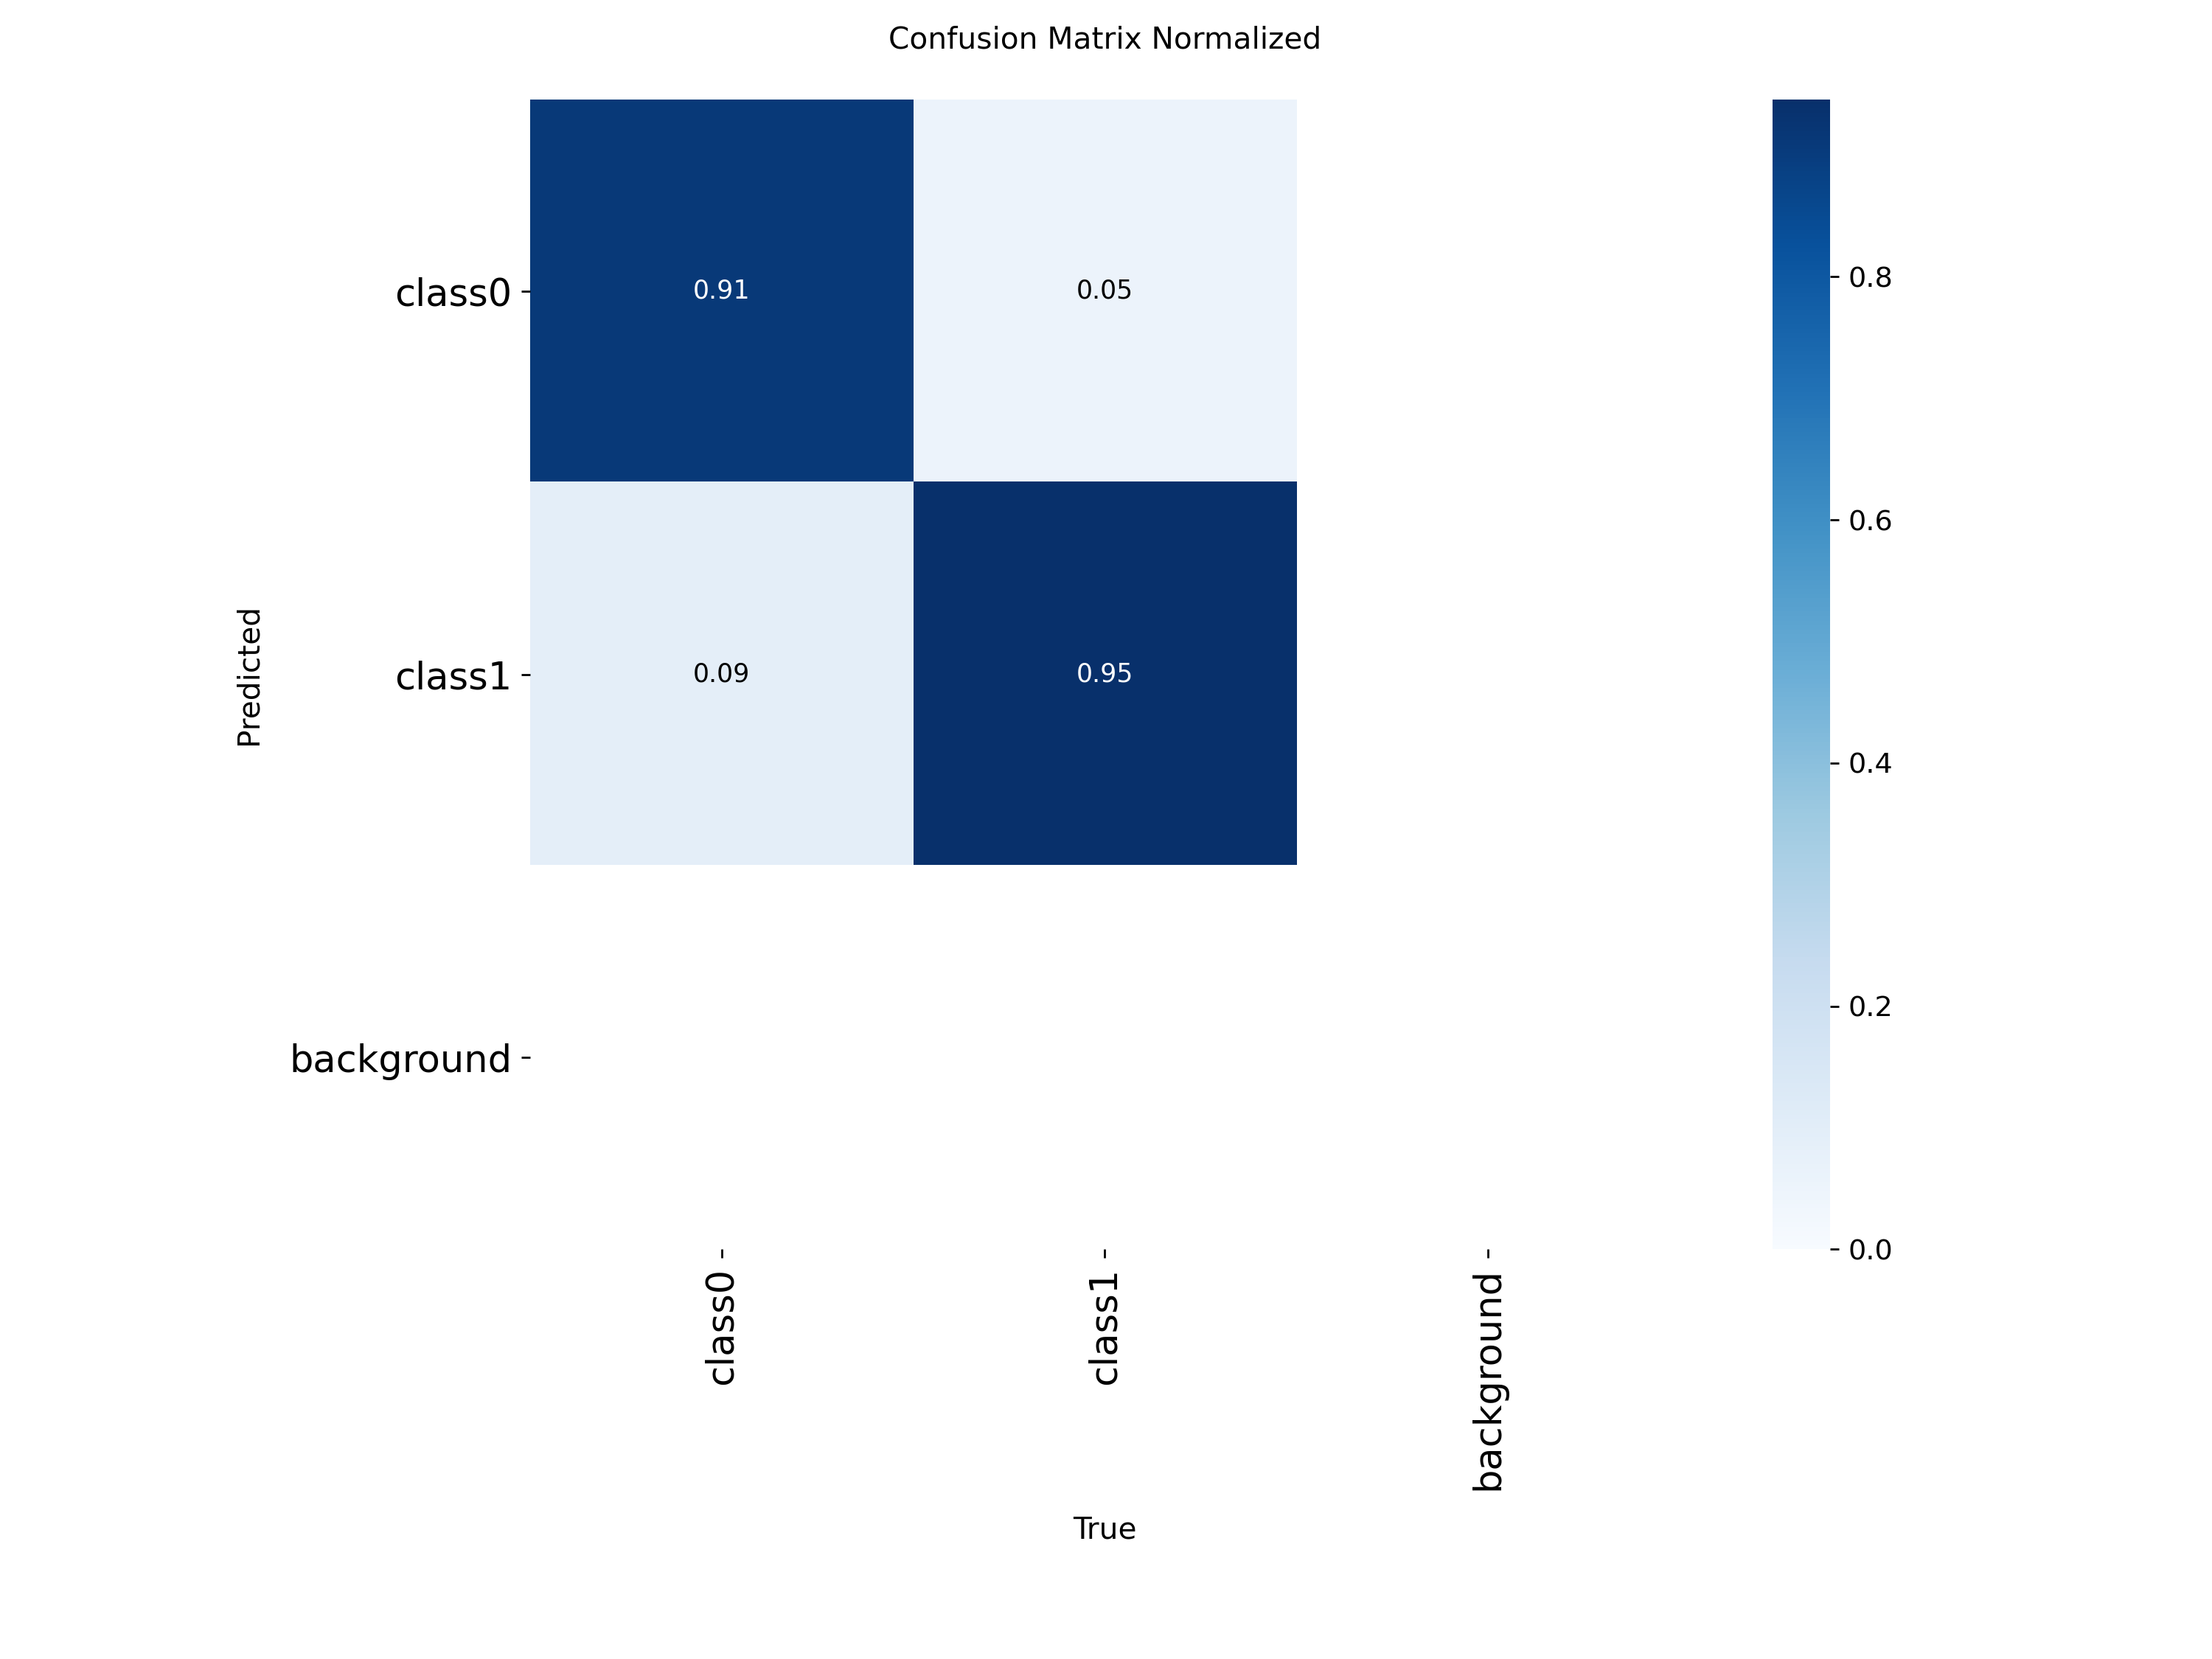
\includegraphics[width=0.80\linewidth]{./imgs/t5-confusion_matrix_normalized.png}
    \caption{Treinamento 5: matriz de confusão normalizada.}
    \label{fig:t5-2}
\end{figure}


\subsection{Treinamento 6 (último)}\label{sec:t6}
Esse foi o último treinamento realizado. As aumentações de dados, a organização das bases de dados, e os parâmetros do modelo utilizados neste treinamento foram resultados dos aprendizados de todos os treinamentos anteriores. Usamos para aumentação de dados rotações individuais das imagens menores e recortes. Para as bases de dados, a base de dados \textit{Fall Video Dataset} foi utilizada exclusivamente para compor o conjuto de treinamento. A base de dados GMDCSA-24 foi utilizada exclusivamente para compor o conjunto de validação. E uma terceira base de dados \textit{Le2i Fall Dataset} foi utilizada exclusivamente para compor o conjunto de teste.


 \begin{figure}[H]
     \centering
     \begin{subfigure}[b]{0.45\linewidth}
         \centering
         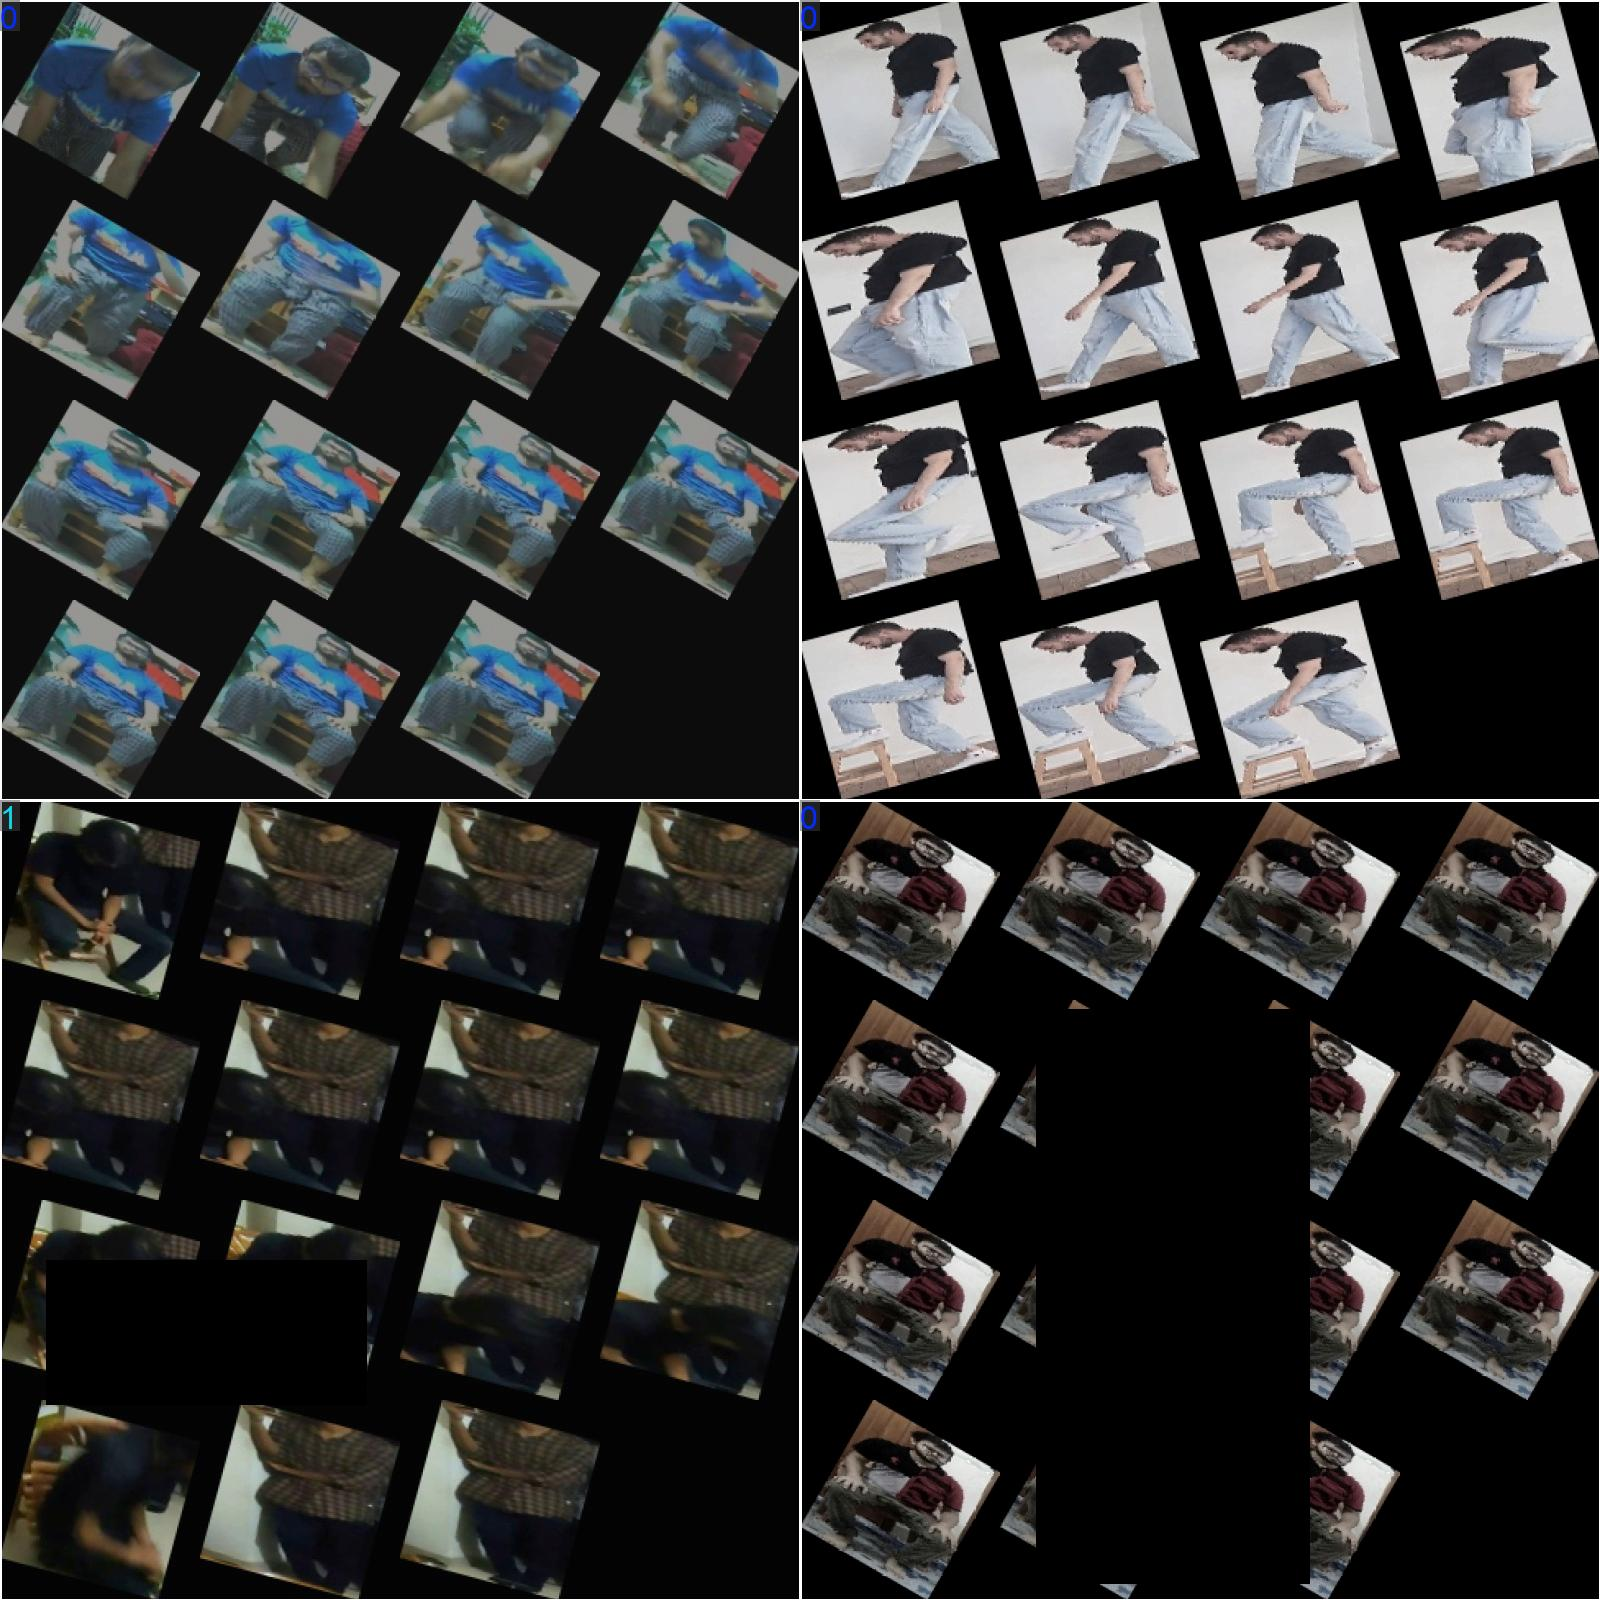
\includegraphics[width=\linewidth]{./imgs/t6-train_batch.jpg}
        \caption{Amostra de batch.}

     \end{subfigure}
     \hspace{0.05\linewidth}
     \begin{subfigure}[b]{0.45\linewidth}
         \centering
         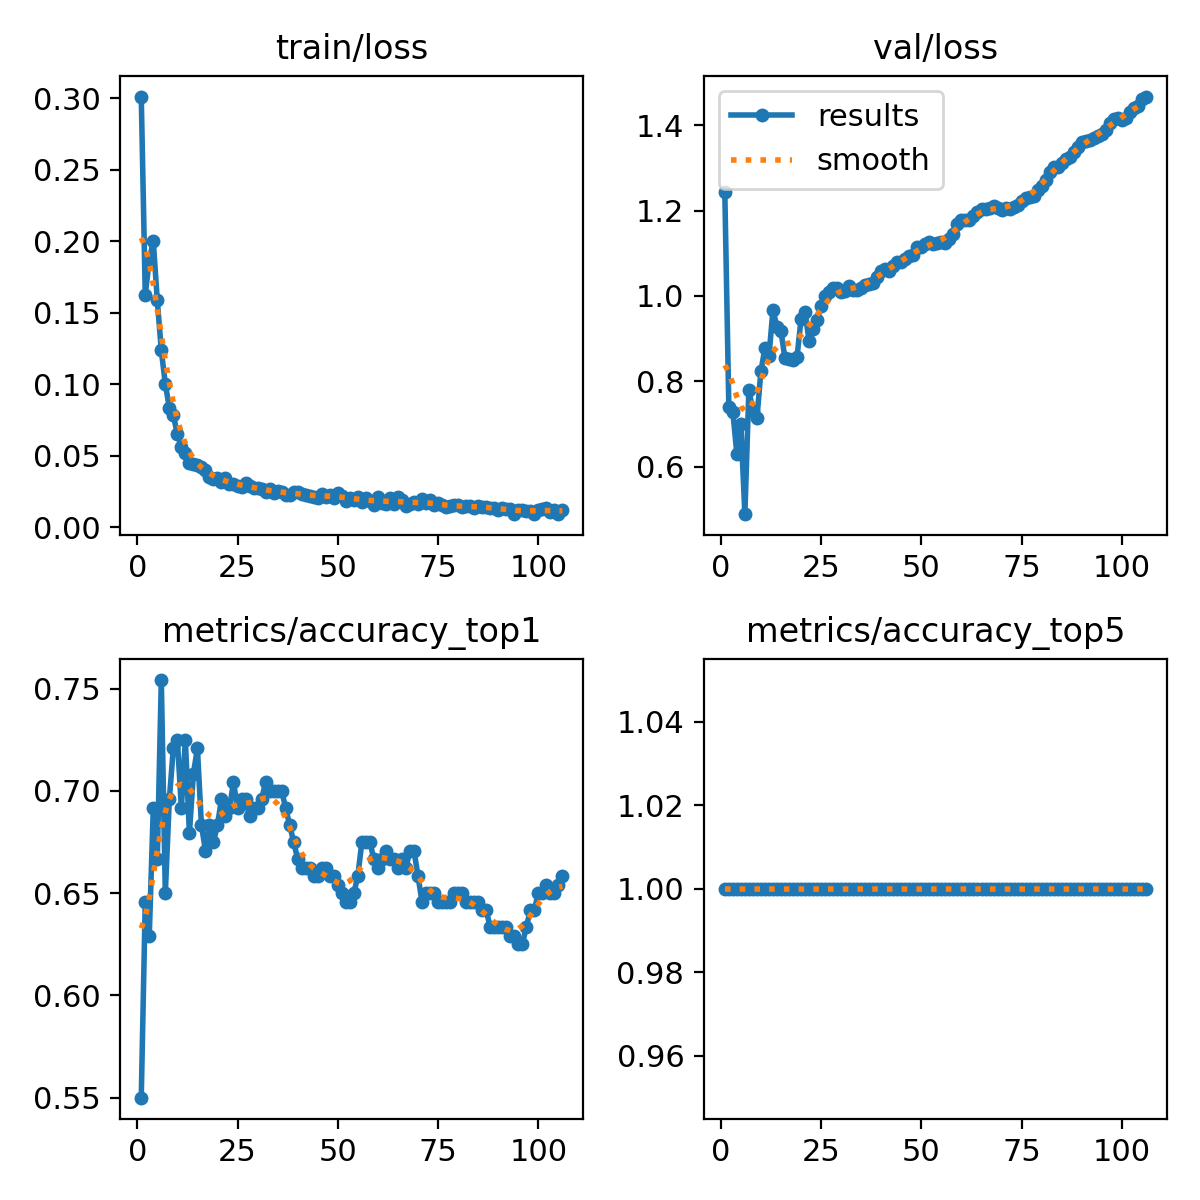
\includegraphics[width=\linewidth]{./imgs/t6-results.png}
        \caption{Métricas de desempenho.}

     \end{subfigure}
    \caption{Treinamento 6: amostra de batch e métricas de desempenho.}
    \label{fig:t6-1}
 \end{figure}

A partir da análise das métricas de desempenho, percebemos que nesse cenário mais desafiador de separação completa entre os dados de treinamento e os dados de validação, os valores da função de perda para os dados de validação começaram a divergir após as épocas iniciais de treinamento. Então, conforme melhor o ajuste do modelo sobre os dados de treinamento, pior seu desempenho sobre os dados de validação (\textbf{Figura \ref{fig:t6-1}}). 

 \begin{figure}[H]
     \centering
     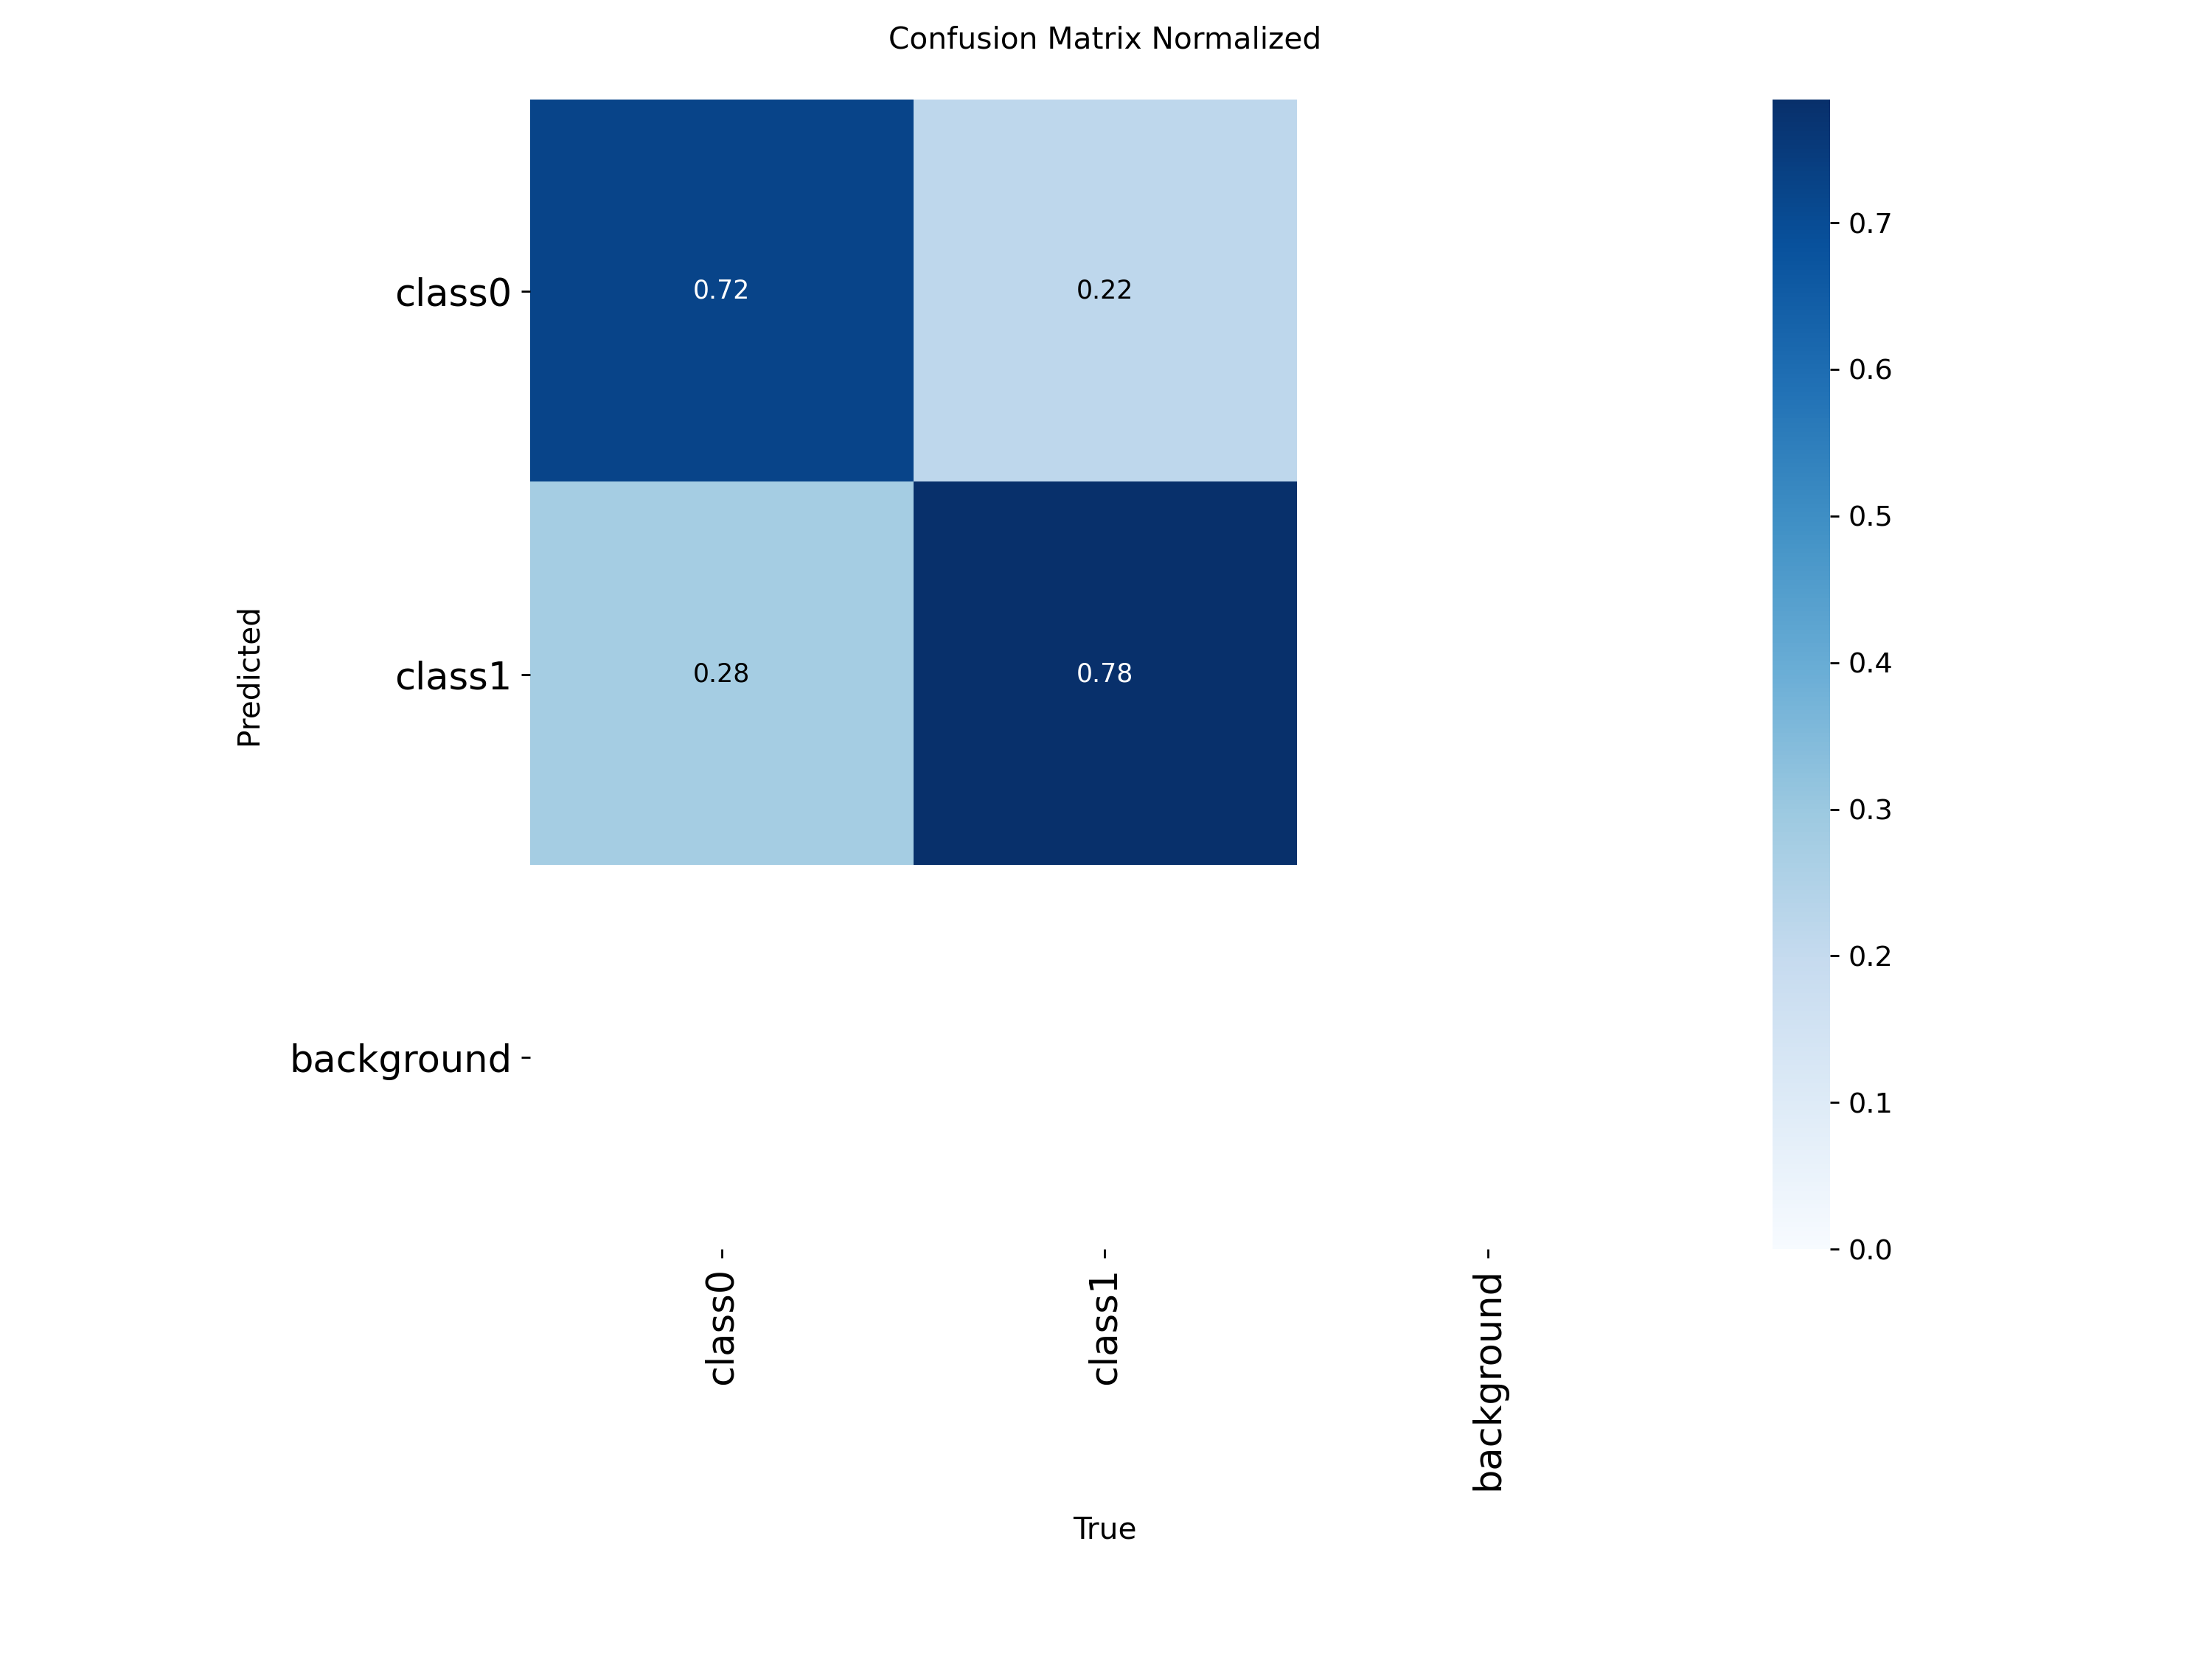
\includegraphics[width=0.80\linewidth]{./imgs/t6-confusion_matrix_normalized.png}
    \caption{Treinamento 6: matriz de confusão normalizada.}
    \label{fig:t6-2}
 \end{figure}

Como esperado, as métricas de desempenho da matriz de confusão normalizada apresentam uma deterioração mais significativa (\textbf{Figura \ref{fig:t6-2}}). 

\subsubsection{Treinamento 6 (último): teste}
Para realizar um levantamento de desempenho do modelo em ambiente de teste, isto é, com dados novos nunca vistos, foi necessário realizar uma flexibilização devido as dificuldades de se trabalhar com vídeos e imagens e dificuldades de se encontrar bases de dados prontas para uso. Nessa flexibilização o teste adquiriu um caráter mais qualitativo e foi realizado da seguinte maneira. Desenvolveu-se um \textit{pipeline} de inferência capaz de simular um fluxo real de processamento de vídeo e classificação da condição de queda ou de não queda. Esse fluxo real de processamento foi aplicado sobre a base de dados \textit{Le2i Fall Dataset}. Os resultados estão consolidados em gifs que podem ser verificados pelo seguinte link:  \url{https://drive.google.com/drive/folders/1_UFfdm8RTmJ9JB9qiaWrywma39UExQ5Q?usp=drive_link}. 

Então, aqui, apresentaremos algumas imagens que permitem ao leitor ter uma ideia do desempenho da rede treinada (para uma compreensão maior, olhar repositório de gif mencionado anteriormente). Essas imagens estão apresentadas nas \textbf{Figuras \ref{fig:teste-1}, \ref{fig:teste-2} e \ref{fig:teste-3}}. As discussões dessas imagens acontecem na seção de discussão apresentada a seguir.



\begin{figure}[H]
	\centering
	% --- First row ---
	\begin{subfigure}[b]{0.45\linewidth}
		\centering
		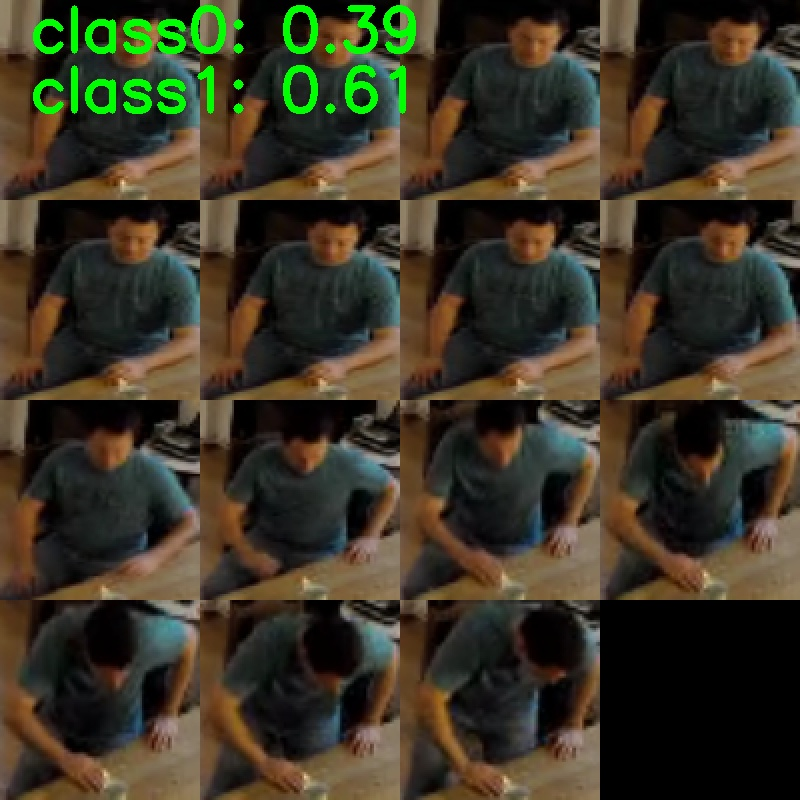
\includegraphics[width=\linewidth]{./imgs/teste1/frame_infer_00015.jpg}
	\end{subfigure}
	\hspace{0.05\linewidth}
	\begin{subfigure}[b]{0.45\linewidth}
		\centering
		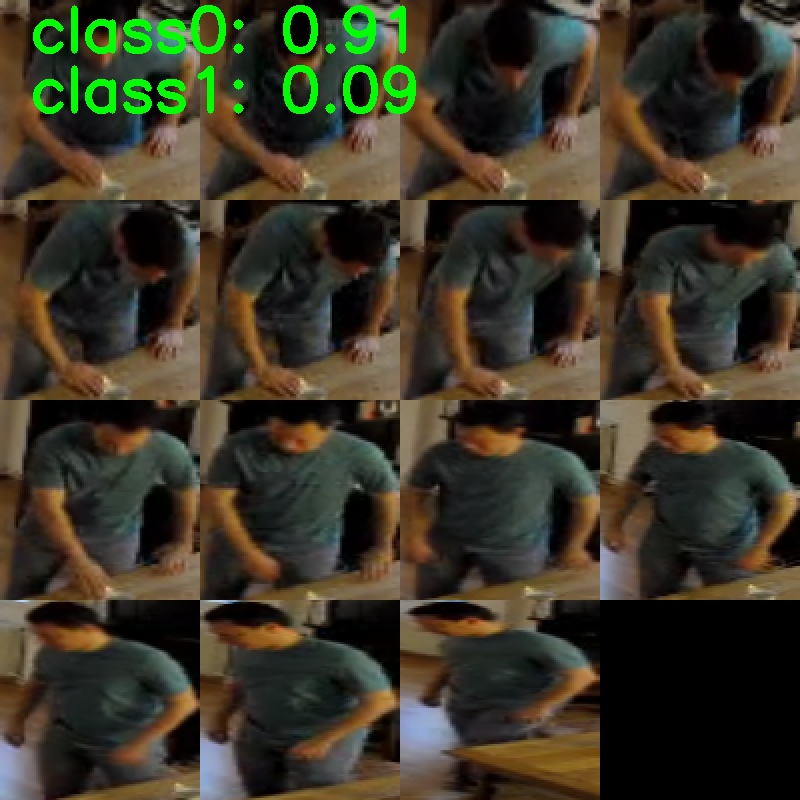
\includegraphics[width=\linewidth]{./imgs/teste1/frame_infer_00025.jpg}
	\end{subfigure}
	
	\vspace{0.5cm} % space between rows
	
	% --- Second row ---
	\begin{subfigure}[b]{0.45\linewidth}
		\centering
		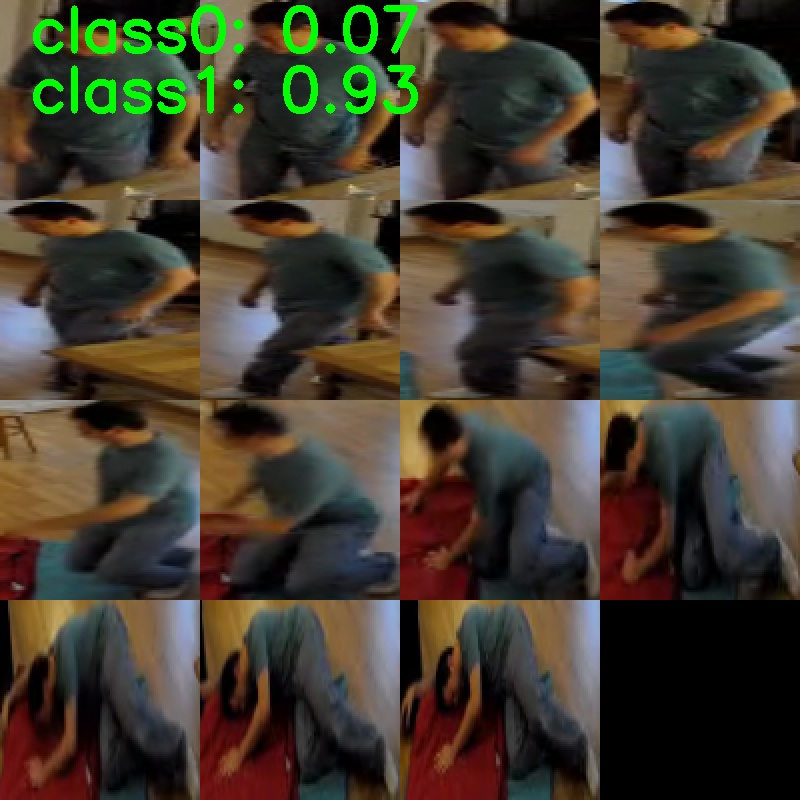
\includegraphics[width=\linewidth]{./imgs/teste1/frame_infer_00035.jpg}
	\end{subfigure}
	\hspace{0.05\linewidth}
	\begin{subfigure}[b]{0.45\linewidth}
		\centering
		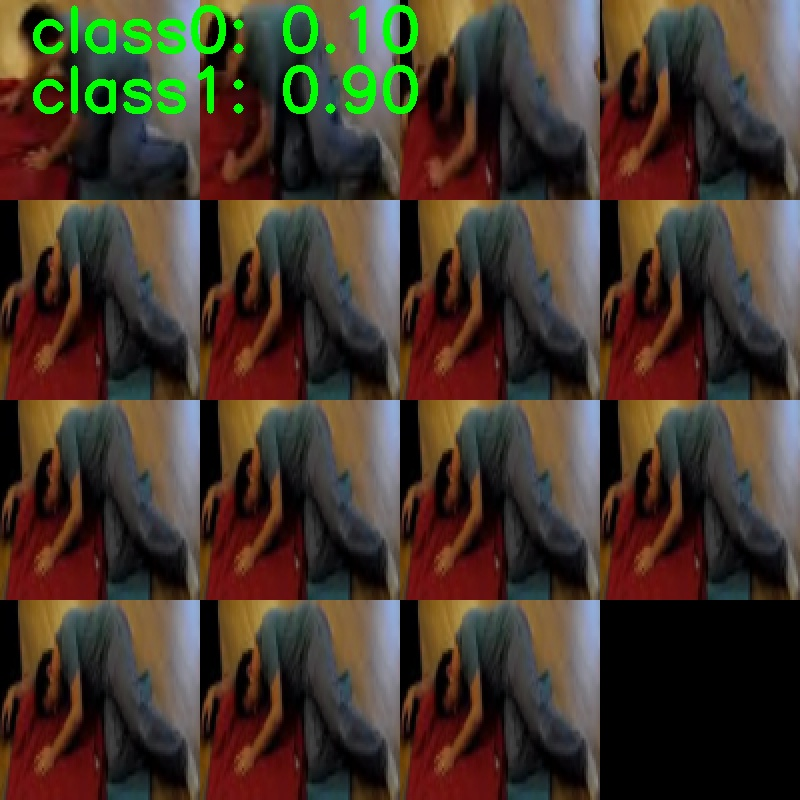
\includegraphics[width=\linewidth]{./imgs/teste1/frame_infer_00045.jpg}
	\end{subfigure}
	
	\caption{Amostra 1 de imagens de uma simulação de fluxo real de aplicação da solução de detecção de queda para realização de teste qualitativo do modelo treinado.}
	\label{fig:teste-1}
\end{figure}



\begin{figure}[H]
	\centering
	% --- First row ---
	\begin{subfigure}[b]{0.45\linewidth}
		\centering
		
\includegraphics[width=\linewidth]{./imgs/teste2/frame_infer_00015.jpg}
	\end{subfigure}
	\hspace{0.05\linewidth}
	\begin{subfigure}[b]{0.45\linewidth}
		\centering
		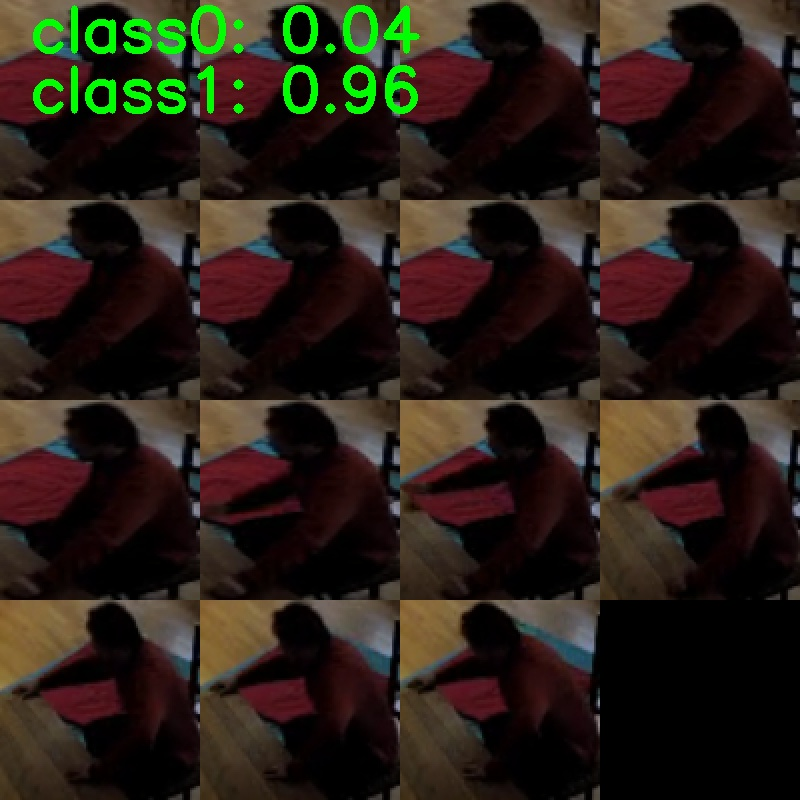
\includegraphics[width=\linewidth]{./imgs/teste2/frame_infer_00020.jpg}
	\end{subfigure}
	
	\vspace{0.5cm} % space between rows
	
	% --- Second row ---
	\begin{subfigure}[b]{0.45\linewidth}
		\centering
		
\includegraphics[width=\linewidth]{./imgs/teste2/frame_infer_00025.jpg}
	\end{subfigure}
	\hspace{0.05\linewidth}
	\begin{subfigure}[b]{0.45\linewidth}
		\centering
		
\includegraphics[width=\linewidth]{./imgs/teste2/frame_infer_00035.jpg}
	\end{subfigure}
	
	\caption{Amostra 2 de imagens de uma simulação de fluxo real de aplicação da solução de detecção de queda para realização de teste qualitativo do modelo treinado.}
	\label{fig:teste-2}
\end{figure}


\begin{figure}[H]
	\centering
	% --- First row ---
	\begin{subfigure}[b]{0.45\linewidth}
		\centering
		
\includegraphics[width=\linewidth]{./imgs/teste3/frame_infer_00015.jpg}
	\end{subfigure}
	\hspace{0.05\linewidth}
	\begin{subfigure}[b]{0.45\linewidth}
		\centering
		
\includegraphics[width=\linewidth]{./imgs/teste3/frame_infer_00025.jpg}
	\end{subfigure}
	
	\vspace{0.5cm} % space between rows
	
	% --- Second row ---
	\begin{subfigure}[b]{0.45\linewidth}
		\centering
		
\includegraphics[width=\linewidth]{./imgs/teste3/frame_infer_00035.jpg}
	\end{subfigure}
	\hspace{0.05\linewidth}
	\begin{subfigure}[b]{0.45\linewidth}
		\centering
		
\includegraphics[width=\linewidth]{./imgs/teste3/frame_infer_00045.jpg}
	\end{subfigure}
	
	\caption{Amostra 3 de imagens de uma simulação de fluxo real de aplicação da solução de detecção de queda para realização de teste qualitativo do modelo treinado.}
	\label{fig:teste-3}
\end{figure}


\subsubsection{Treinamento 6 (último): discussão}
Dentro do que foi apresentado e a partir da perspectiva dos autores, é relevante discutir questões de qualidade das bases de dados, desempenho do modelo durante o treinamento e desempenho do melhor modelo durante o teste qualitativo. Sobre as bases de dados, pode-se afirmar que encontrá-las em abundância adequada é um desafio. Além disso, quando encontradas, as bases de dados não estão prontas para uso. Elas precisam ser processadas de modo que as situações de queda e de não queda sejam localizadas com precisão nos vídeos. Ressaltar a condição de escassez das bases de dados assim como de necessidade de pré-procesamento delas é importante uma vez que acredita-se que a principal carência do sistema de detecção de queda desenvolvido vem dos seus dados de treinamento, teste, e validação. Com mais dados capazes de varrer mais situações de queda e de não queda e com um processo mais cuidadoso de rotualação é muito provável que o modelo conseguiria classificar com melhor precisão as situações de queda e de não queda.

Sobre o desempenho do modelo ao longo de todos os treinamentos, é importante destacar as dificuldades de se utilizar as métricas de redução dos valores das funções de perda como uma referência absoluta de melhora de desempenho do modelo. É importante ter ciência que esses valores apresentam melhor serventia dentro de uma perspectiva qualitativa onde deseja-se ter um panorama das evolução do treinamento, da convergência do modelo e de possíveis condições de \textit{overfitting} e de vazamento de dados. No caso particular desse trabalho, as informações da função de perda sobre os dados de validação é importante ao fornecer uma indicação que a quantidade de dados utilizados está insuficiente para o problema de classificação sobre imagens abordado. Essa indicação vem da rápida convergência do modelo dentro dos valores da função de perda de validação indicando que o modelo já não tem muito mais o que aprender: com mais dados, mais situações de queda e de não queda, acreditá-se que essa convergência deveria ser mais lenta.

Sobre o desempenho do modelo dentro dos testes qualitativos, verifica-se de imediato a importância da realização de testes com dados fora do conjunto de treinamento e validação. É partir dos dados de teste que pode-se ter uma segurança melhor do desempenho do modelo. No caso deste trabalho, o desempenho do modelo pela matriz de confusão dos dados de validação não se sustentou no teste qualitativo. A partir do teste qualitativo percebe-se que o modelo ficou enviesado para a situação de queda, classificando preciptadamente muitas situações que não são queda como sendo de queda (\textbf{Figuras \ref{fig:teste-2} e \ref{fig:teste-3}}). 



\section{Conclusão}\label{sec:conc}
Diante do apresentado, é possível concluir que o treinamento de um classificador binário capaz de trabalhar com imagens para classificação de situações de queda e de não queda foi desenvolvido. Todas as principais etapas para o treinamento de um modelo foram desenvolvidas: obtação da base de dados, preparação da base de dados, separação da base de dados; aumentação da base de dados, escolha do otimizador, da função de perda e dos hiper-parâmetros; treinamento do modelo, levantamento de curvas de desempenho durante o treinamento, levantamento da matriz de confusão e realização de desempenho sobre dados de teste.

O trabalho também envidênciou que o maior custo no processo de treinamento de um modelo de inteligência artificial está nas atividades relativas a obtenção e manipulação dos dados.

Por fim, um modelo capaz de classificar uma situação de queda e não queda foi desenvolvido e testado. Esse modelo sustentado por uma arquitetura de redes neurais convolucionais foi capaz, dentro das suas limitações, de reconhecer as relações temporais existentes na imagem de entrada para realizar sua classificação. Apesar do seu desempenho não ter se destacado, há um entendimento dos autores que as ideias utilizadas neste trabalho foram validadas com sucesso de modo que com mais tempo e um trabalho mais atento no processo de organização da base de dados acredita-se que seria possível desenvolver um bom classificador de queda e de não queda baseado em redes neurais convolucionais.

% Estes comandos definem o finall do texto. Não tire eles daqui!
\bibliographystyle{sbc}
\bibliography{sbc-template}

\end{document}
